\documentclass[a4,english]{report}
\usepackage[a4paper, hmargin=2.5cm,vmargin=1.5cm]{geometry}
\usepackage[colorlinks = true]{hyperref}
\hypersetup{
  pdftitle    = {Master thesis - Feedback on Backpressure},
  pdfauthor   = {Richard van Heest},
  colorlinks  = true,
  linkcolor   = [rgb]{0.1,0.1,0.4},
  citecolor   = [rgb]{0.4,0.1,0.1},
  filecolor   = [rgb]{0.1,0.4,0.4},
  urlcolor    = [rgb]{0.1,0.1,0.7}
}
\usepackage{listings}
\usepackage{color}
\usepackage{verbatim} % \verb{} for inline code
\usepackage[numbers,square,sort]{natbib} % references as [1,2,3] in superscript -> see also http://merkel.zoneo.net/Latex/natbib.php
\usepackage{xspace} % put a space after an abbreviation in a newcommand
\usepackage{amsmath}
\usepackage{amsfonts} % for the \checkmark command
\usepackage{pifont}% http://ctan.org/pkg/pifont
\usepackage{graphicx} % to show images
\usepackage{float} % places the images at precisely the location in the LaTeX code
\usepackage[bottom]{footmisc} % fix \footnote{} position at the bottom of the page
\usepackage{datetime}
\usepackage{caption} % used for multiple images in one figure
\usepackage{subcaption} % used for multiple images in one figure
\usepackage[nameinlink]{cleveref}
\usepackage[titletoc, page]{appendix}

\newdateformat{monthyeardate}{\monthname[\THEMONTH], \THEYEAR}

\crefname{appsec}{Appendix}{Appendices}

%\newcommand{\todo}[1]{\textcolor{red}{\textbf{\large @TODO: #1}}}
\newcommand{\code}[1]{\sloppy{\mbox{\texttt{#1}}}}
\newcommand{\HRule}{\rule{\textwidth}{0.5mm}}

\newcommand{\obs}{\texttt{Observable}\xspace}
\newcommand{\obv}{\texttt{Observer}\xspace}
\newcommand{\subs}{\texttt{Subscription}\xspace}
\newcommand{\subj}{\texttt{Subject}\xspace}
\newcommand{\bsubj}{\texttt{BehaviorSubject}\xspace}
\newcommand{\sch}{\texttt{Scheduler}\xspace}
\newcommand{\ier}{\texttt{IEnumerator}\xspace}
\newcommand{\ieb}{\texttt{IEnumerable}\xspace}
\newcommand{\id}{\texttt{IDisposable}\xspace}
\newcommand{\itr}{\texttt{Iterator}\xspace}
\newcommand{\itb}{\texttt{Iterable}\xspace}
\newcommand{\comp}{\texttt{Component}\xspace}

\definecolor{pgreen}{rgb}{0,0.5,0}
\definecolor{pgrey}{rgb}{0.5,0.5,0.5}
\definecolor{mauve}{rgb}{0.58,0,0.82}
\lstdefinestyle{ScalaStyle}{
  frame=tb,
  language=Scala,
  showspaces=false,
  showtabs=false,
  breaklines=true,
  showstringspaces=false,
  breakatwhitespace=true,
  commentstyle=\color{pgreen},
  keywordstyle=\color{blue},
  stringstyle=\color{mauve},
  basicstyle=\ttfamily,
  moredelim=[il][\textcolor{pgrey}]{$$},
  moredelim=[is][\textcolor{pgrey}]{\%\%}{\%\%},
  numbers=left,
  numberstyle=\color{pgrey},
  columns=flexible,
  mathescape=true,
  escapechar=|
}
\lstdefinestyle{InlineScalaStyle}{
  frame=none,
  language=Scala,
  xleftmargin=.25in,
  xrightmargin=.25in,
  showspaces=false,
  showtabs=false,
  breaklines=true,
  showstringspaces=false,
  breakatwhitespace=true,
  commentstyle=\color{pgreen},
  keywordstyle=\color{blue},
  stringstyle=\color{mauve},
  basicstyle=\ttfamily,
  moredelim=[il][\textcolor{pgrey}]{$$},
  moredelim=[is][\textcolor{pgrey}]{\%\%}{\%\%},
  numbers=none,
  columns=flexible,
  mathescape=true,
  escapechar=|
}
\lstdefinestyle{HaskellStyle}{
  frame=tb,
  language=Haskell,
  showspaces=false,
  showtabs=false,
  breaklines=true,
  showstringspaces=false,
  breakatwhitespace=true,
  commentstyle=\color{pgreen},
  keywordstyle=\color{blue},
  stringstyle=\color{mauve},
  basicstyle=\ttfamily,
  moredelim=[il][\textcolor{pgrey}]{$$},
  moredelim=[is][\textcolor{pgrey}]{\%\%}{\%\%},
  numbers=left,
  numberstyle=\color{pgrey},
  columns=flexible,
  mathescape=true,
  escapechar=|,
  deletekeywords={Monad, Functor, flip, return, Int, const}
}
\lstdefinestyle{InlineHaskellStyle}{
  frame=none,
  language=Haskell,
  xleftmargin=.25in,
  xrightmargin=.25in,
  showspaces=false,
  showtabs=false,
  breaklines=true,
  showstringspaces=false,
  breakatwhitespace=true,
  commentstyle=\color{pgreen},
  keywordstyle=\color{blue},
  stringstyle=\color{mauve},
  basicstyle=\ttfamily,
  moredelim=[il][\textcolor{pgrey}]{$$},
  moredelim=[is][\textcolor{pgrey}]{\%\%}{\%\%},
  numbers=none,
  columns=flexible,
  mathescape=true,
  escapechar=|,
  deletekeywords={Monad, Functor, flip, return, Int, const}
}

\begin{document}
\begin{titlepage}
\begin{center}
\textsc{\Large Delft University of Technology}\\[0.5cm]
\textsc{\LARGE Master thesis}\\[0.5cm]
{\huge \bfseries \todo{title of the thesis here}}

\HRule \\[3.0cm]

\begin{tabular}{l r}
	\begin{minipage}{0.5\textwidth}
	\begin{flushleft}
	\large
	\emph{Author:}\\
	Richard \textsc{van Heest} (std. nr. 4086570)\\
	\end{flushleft}
	\end{minipage}
	&
	\begin{minipage}{0.464\textwidth}
	\begin{flushright}
	\large
	\emph{Thesis committee:}\\
	Prof. dr. H.J.M. \textsc{Meijer}\\
	\todo{other members of the thesis committee here}
	\end{flushright}
	\end{minipage}
\end{tabular}

\vfill
\textsc{\large \today}

\todo{TU Delft ( + logo), EEMCS, [Master Program], [Chosen Specialization]}\\
\todo{Applied Duality???}
\end{center}
\end{titlepage}

\pagestyle{plain}
\pagenumbering{roman}
\setcounter{page}{1}
\chapter*{Acknowledgment}

I would like to thank Erik Meijer, my supervisor during this thesis project, for all his support, enthusiasm and hacker mentality. \textit{Erik, it was an honor to receive an email in May 2014, asking whether I was interested in doing my master thesis with you. From the beginning it was clear to both of us that Reactive Programming and Rx were a shared interest. It was great working with you on RxMobile, which has turned out to be very useful for this thesis. You really inspired me to have a hacker mentality, always keep trying to get things working and to never give up. I sincerely hope the completion of this thesis will not be the \code{onCompleted} event on the stream of our collaborations, but instead will just be the \code{onNext} event of a finished project on a much longer stream!}

I also want to thank Georgios Gousios and Arie van Deursen for taking their time to be part of my thesis committee and providing me with great feedback.

Furthermore, I would like to thank my fellow students and friends at TU Delft, Eddy Bertoluzzo, Georgi Khomeriki, Mircea Voda, Mike de Waard and Lars Willems, who were doing their master theses in parallel with me. Thanks for the great time we had together at EWI-HB 08.250 and the many discussions at the whiteboard and at Hangouts/Skype!

A special thanks to Michel van Heest, my brother, for creating all the diagrams in this thesis.

Finally, I would like to thank my family, friends and colleagues for their support and interest in my thesis work, even though most of them still don't understand a word of what will follow in the rest of this thesis!

\begin{flushright}
Richard van \textsc{Heest}\\
\textit{Middelharnis, The Netherlands}\\
\textit{\monthyeardate\today}
\end{flushright}

\clearpage
\setcounter{tocdepth}{1}
{\hypersetup{linkcolor = black} \tableofcontents}

\clearpage
\setcounter{page}{1}
\setcounter{chapter}{-1}
\pagenumbering{arabic}
\chapter*{Introduction}
\addcontentsline{toc}{chapter}{Introduction}

Reactive programming is a paradigm in which the program observes events that occur in its environment and reacts to these events as they occur. This is in contrast to the more familiar interactive program flow in which a program \emph{requests} some form of data and only continues the program flow once this data is received. Instead of pulling data in the usual interactive way, reactive programs get data (or events) pushed to them on which they respond according to the program. Some of the most common usages of reactive programming can be found in user interfaces (mouse moves, key events or button presses), network communication, database queries and clocks or timers \cite{meijer2012-YMIAD}.

In an interactive program, the \textit{consumer} is in charge of requesting the data. The \textit{producer} only has to obey the commands from the consumer and return the requested data. In reactive programs this is the exact opposite: the producer is in charge and sends the data \emph{at its own pace} \cite{berry1991-Reactive}, whereas the consumer has to react to the data it receives from the producer.

This shift in roles between producer and consumer poses an interesting problem: ``\textit{What happens when the consumer cannot keep up with the amount of data that is sent by the producer?}''. In other words, when a consumer has to deal with an overproducing source, how can it handle the excessive amount of data? Several solutions with different policies have already been proposed and implemented in order to solve this problem \cite{RxJava-Wiki-Callstack-Blocking,RxJava-Wiki-Backpressure,Reactive-Streams}. We find, however, that some of these work well under certain circumstances but are not suitable for all kinds of reactive programs in general. Other solutions change the contract of reactive programming and put the consumer back into command, but, surprisingly, still call it `reactive'.

This poses the question whether the concepts behind reactive programming have been generalized too much and whether distinctions between different kinds of reactive programs can lead to a clearer view of what solution works best under which conditions. This thesis will discuss this topic extensively in \Cref{chap:problem-statement} and \Cref{chap:exploring-the-problem-space}.

Based on the conclusions of this first part, we will propose a new solution to the overproduction problem, which makes use of control theory and feedback control systems. This solution can be used as a replacement to solutions that put the consumer back in charge.

Feedback control is a technique that is mainly used in mechanical and electrical engineering, but is generally overlooked in computer science. Feedback control can be applied by continuously measuring a system's property, comparing it to a desired value and alter the system's input based on the error between the desired and measured values. The goal is to ultimately bring the measured property as close to the desired value as possible and keep it this way despite external changes that try to bring the system out of balance \cite{janert2013-feedback}.

Although well suited in several use cases, control theory is generally overlooked in computer science and software engineering. To the best of our knowledge, there are even no well-written libraries that allow software developers to construct and run feedback systems in a clean way. As we will use feedback control in our solution for the overproduction problem, we will study the composition of feedback systems in \Cref{chap:intro-to-feedback-control} and present an concise but powerful library for this purpose that is based on the concepts of functional and reactive programming (\Cref{chap:feedback-api}). Using this library, we will then propose our solution to the overproduction problem.

\section*{Research Questions}
\addcontentsline{toc}{section}{Research Questions}
This thesis answers a number of questions that are related to reactive programming, overproducing sources in a reactive context and feedback control, which are listed and briefly introduced in this section.

\subsubsection*{In what ways can a reactive program already be controlled to prevent overproduction?}
There are multiple solutions for controlling overproduction in the context of reactive programming. To understand these solutions we first need to identify the various types of reactive programs and consider their mutual similarities and differences. This is important since the existing solutions do not work for every type of reactive program.

\subsubsection*{How can we implement a \emph{reactive} feedback system that is composed of smaller parts?} 
As the solution to overproduction that is presented in this thesis makes use of control theory and feedback control, and given that these are not yet widely known or used in computer science, it is important to develop an understanding of these techniques and create the tools necessary to construct feedback systems in an easy way. We will show that these can be seen as reactive programs and implement a library on top of existing reactive programming API's.

\subsubsection*{How can the overproduction problem be reduced to a feedback control problem?}
To solve overproduction using feedback control, it is necessary to get out of the context of reactive programming and abstract this into more general problems that can be solved by control theory. Once we develop and solve this more general problem, we can put it back into the context of reactive programs.

\subsubsection*{Can this new solution to overproduction be integrated in an existing API for reactive programming?}
In order for this solution to be useful in practice it is important to be able to interface with existing API's for reactive programming. To test this, a clean API is needed that does not yet implement any solutions for overproduction. For this purpose we use the newly created RxMobile API \cite{RxMobile}.

\section*{Outline}
\addcontentsline{toc}{section}{Outline}
In the next chapter we will continue this thesis report with a short discussion on the definitions of interactive and reactive programming as it is defined in literature (\Cref{chap:problem-statement}). This is followed up with an extensive introduction to a widely used reactive programming API whose concepts have been implemented in many languages. We will discuss the basic principles of this API as well as it's derivation from and relationships with interactive programming interfaces. Once these foundations are laid out, we will give an overview of the different ways in which it tries to overcome overproduction problems. It is important to first gain a good understanding of reactive programming in general and this API especially, since we will build on top of these in the rest of this thesis.

Different circumstances require different approaches to overproduction, as we already hypothesized above. In \Cref{chap:exploring-the-problem-space} we will explore and categorize these circumstances and describe how overproduction is currently best dealt with in each of these situations. Here we also discuss the current state of abstraction over reactive programming and describe our solution to overproduction and explain for which type of reactive programs we think this will apply.

As we will use control theory to solve the problem of overproduction, and given that this topic is not well known in computer science we will briefly introduce this topic in \Cref{chap:intro-to-feedback-control}. We also provide an extended example of a simple way to apply feedback control. This example is further used to briefly demonstrate some of the difficulties we currently experience with setting up and tuning a feedback control system.

To the best of our knowledge there does not exist a proper API, library or framework for building and running feedback control systems in production level systems. In \Cref{chap:feedback-api} we derive a simple API for such feedback control systems. This API is based on the concepts of functional and reactive programming and has its basis in the solid foundations of theoretical computer science and category theory. Near the end of this chapter we will return to the example from \Cref{chap:intro-to-feedback-control} and refactor this application such that it uses our newly designed API.

\Cref{chap:solving-overproduction} combines the discussion about overproduction and the theory of feedback control and proposes a new way to deal with overproduction. In this chapter we will reduce this problem to where it can be controlled in an easier way, discuss the various aspects of the resulting feedback system and integrate it in such a way that it can be used as part of a reactive API like RxJava or RxMobile.


\clearpage
\chapter{Programming in a reactive way}
\label{chap:problem-statement}

In order to have a good understanding of what the true meaning and problem of overproduction is, it is important to first of all define what \textit{reactive programming} is, what its relation to other programming patterns is and how this paradigm is implemented in the \textit{Reactive Extensions} API, which will be used throughout this thesis.

In order to understand these fundamental principles, this chapter starts off with defining what reactive programming is, as it is described in the literature. Since this paradigm forms the basis of this whole thesis, it is important to establish the exact notion of reactiveness first.

Then the Reactive Extensions API is discussed. It is the context in which overproduction occurs as well as the basis of the tools we will be using to solve this problem. Since this API is not yet considered to be common knowledge and since not much literature is based on it, we will start from the very basics and discuss all the concepts necessary for this thesis.

At the end of this chapter the overproduction problem is introduces, as well as related work that already provides solutions to this problem.

\section{Reactive Programming}
\label{sec:reactive-programming}
Currently one of the most difficult problems in computer science is handling big amounts of data. No longer are applications bound to the closed world of a single machine and a relational database. Applications these days have access to the whole World Wide Web, exist of large clusters of machines, work with data ranged from SQL-style relational databases to key-value pointer based databases, as well as binary data such as images, audio and video. Also the speed in which data is handled varies from `once a month' to `every millisecond'.

These changes in how applications need to perform require new ways of handling data. No longer is it feasible to load a whole database table into memory for further processing, nor can we permit ourself to wait for all data to be downloaded before we start processing it. Instead we require systems and concepts that are able to handle data right as it gets available to the application, without further delay, preferably in an asynchronous way and without blocking other processes or waiting for all data to have arrived. \cite{meijer2012-YMIAD}

An interesting part of the solution to these problems is Reactive Programming. This term is described by Albert Benveniste and G\'erard Berry in ``\textit{Real time programming: special purpose or general purpose languages}'' \cite{berry1991-Reactive} as he makes a distinction between \textit{interactive} and \textit{reactive} programs:

\begin{quote}
``\textit{Interactive programs} interact at their own speed with users or with other programs; from a user point of view, a time-sharing system is interactive. \textit{Reactive programs} also maintain a continuous interaction with their environment, but \textbf{at a speed which is determined by the environment}, not by the program itself.''
\end{quote}

Reactive programs `observe' events that occur in their environment and react to them as specified by the program. These events can vary from large amounts of data coming in over a network connection or from a database, to mouse moves or other kinds of UI events and from low-latency sensor streams to high-latency calls to web services.

Also notice that Benveniste and Berry explicitly emphasize that that reactive programs run at a speed which is determined by the environment. This means that the producer (which is part of the environment) is in charge of sending data to the consumer. Therefore the consumer (the program) cannot \emph{ask} for new data, it can only \emph{react} to the data that has been sent by the producer. This relationship between producer and consumer is often referred to as \textit{push based behavior}.

A classic example of push based behavior is a mouse pointer moving over the screen. Every time the pointer is moved, it will \emph{push} its new coordinates to the screen, for it to drawn in the new position. From its point of view, the screen \emph{reacts} to the new coordinates being received by the mouse pointer.

This push based behavior is in contrast with the relation between producer and consumer in an interactive program. Here, according to Benveniste and Berry, the consumer (program) interacts on its own speed with its environment. The consumer will determine the speed at which data is transmitted from the outside by continuously asking for the next bit of data. After this is received, the consumer processes the data and then asks for the next piece. This kind of interaction between consumer and producer is often referred to as \textit{pull based behavior}.

One example of a simple interactive program is a foreach-loop iterating over a collection of elements. As long as there are more elements in the collection, it will ask for the next one, process it according to the loop's body and then ask for the next element.

\section{Reactive Extensions}
There have been many attempts to fit the philosophy of reactive programming into libraries, APIs or even languages \cite{ReactiveX, meijer2015-Dart, Reactive-Streams, Akka, Elm, RxMobile}. In this section, we will briefly discuss some of the features of one of these libraries, namely Reactive Extensions (a.k.a. Rx). This project started at Microsoft with an implementation in C\# \cite{meijer2010-Observable} (Rx.Net), was later ported to Java, Scala, Groovy, Kotlin, JavaScript, Swift and many other languages by the open source community \cite{ReactiveX}.

However, these translations have deviated a lot from the original implementation. Most remarkable is that some of them are not even purely `reactive' anymore \cite{meijer2014-Derivation}. Given these deviations from the original paradigm and the state of complexity of these implementations, we decided to use a reference implementation of the original Rx that has recently been written in Scala by Erik Meijer called RxMobile \cite{RxMobile}, with the purpose of creating a light-weight implementation for developing mobile apps on Android. The following discussion and derivation of the API will however apply to both Reactive Extensions and RxMobile and in this section we will therefore refer to both as `Rx'.

\subsection{Core components}
\label{subsec:core-comps}
Rx is a library for composing asynchronous and event based (reactive) programs by using observable sequences. The core of Rx consists of two interfaces: \obs and \obv. The latter can subscribe and react to the events that are emitted by the former. An \obs can emit zero or more events (called \textit{onNext}) and has the possibility to terminate with an \textit{onCompleted} or \textit{onError} event. After either one of these terminal events is emitted, no more events can follow. Therefore the emission protocol can be summarized by the following regular expression: \code{onNext* (onError | onCompleted)?} \cite{MS2010-RxDesign}. When an \obv subscribes to an \obs,  it will return a \subs. With this object reference, one can later unsubscribe from the \obs and clean up potential resources.

\autoref{lst:obs-obv} shows these basic concepts of the \obs, \obv and \subs translated in Scala. Notice that here \subs is a superclass of \obv. Therefore there is no need for the \obs to return a \subs when an \obv subscribes to it. It will however return a \subs when another variant of \code{subscribe} is used, where for example a lambda expression is expected.

\begin{minipage}{\linewidth}
\begin{lstlisting}[style=ScalaStyle, caption={Observable, Observer and Subscription}, label={lst:obs-obv}]
trait Observable[T] {
    def subscribe(observer: Observer[T]): Unit
    def subscribe(onNext: T $\Rightarrow$ Unit): Subscription
    // other variants of subscribe
}

trait Observer[T] extends Subscription {
    def onNext(t: T): Unit
    def onError(e: Throwable): Unit
    def onCompleted(): Unit
}

trait Subscription {
    def isUnsubscribed(): Boolean
    def unsubscribe(): Unit
}
\end{lstlisting}
\end{minipage}

Creating an \obs is done by the \code{Observable.create(Observer $\Rightarrow$ Unit): Observable} method, that takes a lambda expression of type \code{Observer $\Rightarrow$ Unit} and returns an \obs. The input lambda is then used in the implementation of \code{subscribe}, when a \emph{real} \obv is provided. The \obv can be created by supplying it three lambda expressions, one for each kind of event.

\autoref{lst:create-sub-obs} provides a simple example of how both an \obs and \obv are created and used in practice. Here the function in \code{Observable.create} causes the \obs to emit three values and complete afterwards. Notice that these are only emitted after line~\ref{line:subscribe} is executed, when the \obv is subscribed to the \obs. If no one will subscribe, the values will never be produced nor emitted!

\begin{minipage}{\linewidth}
\begin{lstlisting}[style=ScalaStyle, caption={Creating and subscribing to an \obs}, label={lst:create-sub-obs}]
val xs: Observable[Int] $=$ Observable.create((obv: Observer[Int]) $\Rightarrow$ {
    obv.onNext(1)
    obv.onNext(2)
    obv.onNext(3)
    obv.onCompleted()
})
val observer: Observer[Int] $=$ Observer(
    (x: Int) $\Rightarrow$ print(x + " "),
    (e: Throwable) $\Rightarrow$ print(e),
    () $\Rightarrow$ print("completed"))

xs.subscribe(observer) |\label{line:subscribe}|

// result: 1 2 3 completed
\end{lstlisting}
\end{minipage}

Using \code{Observable.create} is a very powerful tool to create an \obs. Many other methods can be derived from it. For example, the \obs in \autoref{lst:create-sub-obs} is often written as \code{Observable.apply(1, 2, 3)}\footnote{In Scala this can be shortened to \code{Observable(1, 2, 3)}. Explicitly writing \code{.apply} is only done for later referral.}. This way of writing is not only more concise and conveys what the true meaning of this expression is in a better way, but it is also exactly the same, since \code{Observable.apply} is implemented in terms of \code{Observable.create}. In fact, all methods that are defined on \obs can be implemented using \code{Observable.create}!

\subsection{Derivation of \obs and \obv}
\label{subsec:derivation}
In 1994, the book `\textit{Design Patterns: Elements of Reusable Object-Oriented Software}' by the \textit{Gang of Four} was published \cite{gamma1994-DesignPatternsGOF}. This book explored the capabilities and pitfalls of object oriented programming and contained an overview of 23 classical software design patterns. Also, the book described the relationships between these 23 design patterns.

One of these design patterns is called the \textit{Observer} pattern and forms the basis of the \obs and \obv interfaces described in the previous section. Even though the Gang of Four did identify a lot of relations between the different design patterns, it failed to identify any relation between the Observer pattern and any other pattern, except for the Mediator pattern.

\begin{figure}[H]
	\begin{center}
		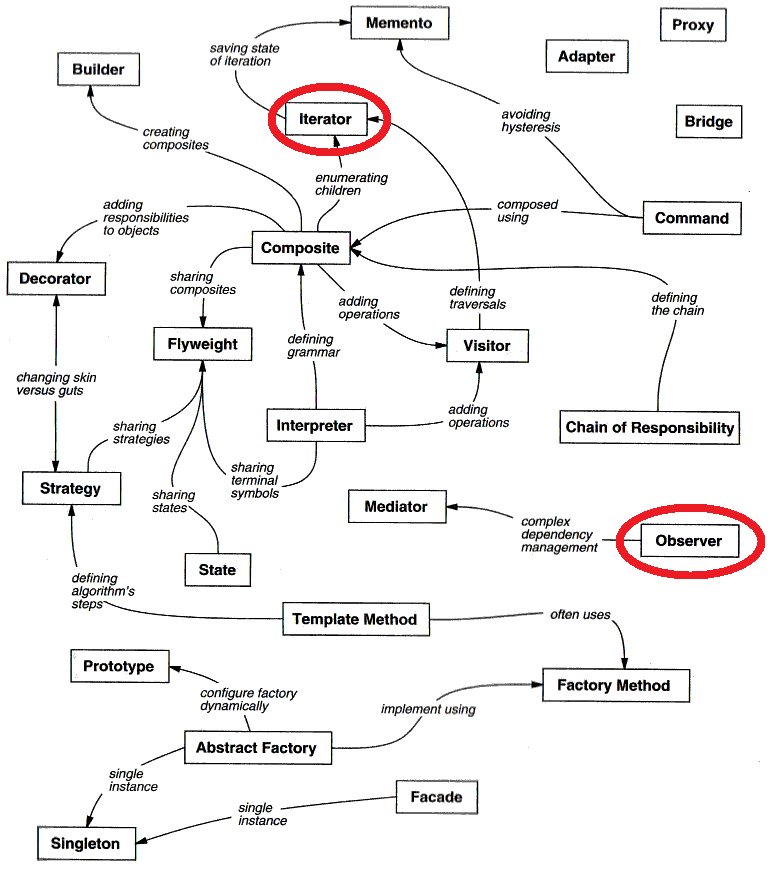
\includegraphics[width=0.48\textwidth]{figures/DesignPatternRelationships_bew.png}
	\end{center}
	\label{fig:designPatternRelationships}
	\caption{Relations between design patterns according to \cite{gamma1994-DesignPatternsGOF}}
\end{figure}

In 2010, Erik Meijer published a short paper called `\textit{Subject/Observer is Dual to Iterator}' \cite{meijer2010-Observable}, where he described a mathematical relationship between the Observer pattern and the Iterator pattern based on categorical duality. The paper shows that instances of the Observer pattern can be viewed as push-based collections, rather than the pull-based collections that result from the Iterator pattern. For later parts of this thesis, it is important to understand the mathematical basis of this relationship between the \obs and \obv interfaces in Rx and the \ieb and \ier interfaces in the Iterator pattern\footnote{For the purpose of the upcoming derivation we have chosen the C\# naming conventions of the Iterator pattern. In other programming languages these interfaces are respectively known as \code{Iterable} and \code{Iterator}.} (see \autoref{lst:itb-itr}).

In most common languages \ieb forms the basis of the Collections API. It has only one method \code{getEnumerator} that returns the \ier to iterate over the elements in the collection. The \ier interface on the other hand contains two methods to be implemented: \code{moveNext} and \code{current}. The former performs a side effect by moving a pointer to the next element in the iteration and then returns a \code{Boolean} to indicate whether or not there was a next element. The latter is a pure function that just returns the element the pointer is currently pointing to. Notice that the \code{moveNext} method can throw an exception rather than returning \code{false} in case an error occurs.

Besides providing these two methods, \ier in \autoref{lst:itb-itr} also extends the \id interface. This interface is meant to signal to the \ieb that no more elements will be pulled and that it can `start collaborating' with the garbage collector to clean up resources. The real meaning of \ier extending \id however, is that \code{getEnumerator} not only returns an \ier, but also returns something that is disposable. The \id interface is therefore not really part of \ier but rather a part of what \code{getEnumerator} returns \cite{E2E-Rx}. For now we will consider \id to be a silent bystander that is will be ignored in the derivation.

\begin{minipage}{\linewidth}
\begin{lstlisting}[style=ScalaStyle, caption={\ieb and \ier interfaces}, label={lst:itb-itr}]
trait IEnumerable[T] {
    def getEnumerator(): IEnumerator[T]
}
trait IEnumerator[T] extends IDisposable {
    def moveNext(): Boolean // throws Exception
    def current: T
}
trait IDisplosable {
    def dispose(): Unit
}
\end{lstlisting}
\end{minipage}

These two interfaces together form the basis of all pull-based or interactive collections as described in \autoref{sec:reactive-programming}. The user asks for the next element and will (eventually) get one in case a next element can be produced. In the following we will transform these interfaces for pull-based collections into interfaces for push-based or reactive collection, where the user subscribes to a collection and receives data once it is produced. This derivation, as well as its conclusion that interactive and reactive collections are each other's dual, is based on some categorical transformations and are discussed in several papers, as well as several keynotes and Channel9 video's \cite{meijer2010-Observable, meijer2012-YMIAD, E2E-Rx, meijer2014-Duality-And-The-End-Of-Reactive}. This derivation, as well as some of the intermediate steps are important for later parts of this thesis.

The first step in this derivation is to rewrite the two methods in the \ier interface into a single method \code{getNext()}. Using the categorical \textit{coproduct} \cite{rydeheard1988-Category-Theory} we can combine these two methods and determine its type signature: \code{getNext()} can either fail with an exception or succeed with either an element or no element, resulting in the type signature \code{getNext(): Try[Option[T]]}. The new, intermediate, set of interfaces is shown in \autoref{lst:itb-itr-interm}.

\begin{minipage}{\linewidth}
\begin{lstlisting}[style=ScalaStyle, caption={\ier interface after applying coproduct}, label={lst:itb-itr-interm}]
trait IEnumerable[T] {
    def getEnumerator(): IEnumerator[T]
}
trait IEnumerator[T] {
    def getNext(): Try[Option[T]]
}
\end{lstlisting}
\end{minipage}

Since both interfaces now only have one single method, and given that the only purpose of \ieb is to produce an \ier, they can be written as a single lambda expression. An \ieb can be written as:

\begin{equation} \label{eq:itb}
\code{() $\Rightarrow$ (() $\Rightarrow$ Try[Option[T]])}
\end{equation}

Notice that applying \code{Unit} to the outer lambda yields another lambda expression, which corresponds to the type signature of \code{getNext} in \autoref{lst:itb-itr-interm}: \code{() $\Rightarrow$ Try[Option[T]]}.

The next step in this transformation is to dualize \cite{rydeheard1988-Category-Theory} lambda~expression~\ref{eq:itb}. A very informal way of describing duality is to flip all the arrows and rewrite the lambda expression. For example, the duality of $f :: A \rightarrow B$ is $\bar{f} :: A \leftarrow B \equiv B \rightarrow A$. In the same way, we can apply this to lambda~expression~\ref{eq:itb}, resulting in

\begin{equation} \label{eq:obs}
\code{(Try[Option[T]] $\Rightarrow$ ()) $\Rightarrow$ ()}
\end{equation}

This lambda expression takes a lambda from \code{Try[Option[T]]} to \code{Unit}, and returns \code{Unit}.

We can now put this lambda expression back into context by splitting it into two interfaces. The inner lambda \code{Try[Option[T]] $\Rightarrow$ ()} can be rewritten to an interface called \obv, which has one method \code{onNext(t: Try[Option[T]]): Unit}. This method can then be further rewritten into three separate methods by expanding the \code{Try[Option[T]]} type: \code{onNext(t: T): Unit}, \code{onError(e: Throwable): Unit} and \code{onCompleted(): Unit}. The outer lambda on the other hand translates to an interface called \obs, which has one method \code{subscribe(obv: Observer[T]): Unit}. Notice how these interfaces are completely identical to the ones presented in \autoref{lst:obs-obv}.

%So far the presence of \id has been ignored in this derivation. This interface can however be found in \autoref{lst:obs-obv}, renamed as \subs. \todo{Add a couple of words on the functionality of \id and \subs and how they are the same.}

So far, the presence of \id has been ignored in this whole derivation. The reason for that is that this interface is considered to be a \emph{second} thing that is returned by the \ieb, rather than a supertype of \ier. What therefore basically happened in the derivation is that we only dualized the enumerator\textit{ness} and left the disposable\textit{ness} out of the dualization process \cite{E2E-Rx}. Therefore the dualized \ier, now called \obv, still extends from \id, even though this only means that we pass \textit{two} arguments to the \code{Observable.subscribe(obv: Observer)}. Just as the \id was meant to signal to the \ieb that no more elements will be polled and that it can clean up its resources, now \id signals to the \obs that it should stop sending data to the \obv. Finally, \id is renamed to \subs and its method \code{dispose} is split into two methods \code{unsubscribe} and \code{isUnsubscribed}.

% really dualized the enumeratorNESS but not the disposableNESS
% \ieb returned \ier AND \id
% now we dualized the enumeratorNESS, \id remained, so we need to return \id in \obs instead of void
% so when we subscribe to an \obs with an \obv, we get back a \id to unsubscribe later

This derivation shows that interactive, pull-based collections are the mathematical dual of reactive, push-based collections. The \obs and \obv interfaces can directly be derived from the \ieb and \ier interfaces. Both sets of interfaces can therefore be considered to be collections. In other words: streaming data behaves exactly the same way as regular collections, such as arrays, lists and sets, except for them being push-based rather than pull-based \cite{meijer2012-YMIAD, meijer2010-Observable}. In the world of push-based collections one \emph{subscribes} to the stream in order to \emph{react} to the next element that is being send, whereas one \emph{asks} for the next element in a pull-based scenario.

\subsection{\obs as a monad}
\label{subsec:obs-monad}
As described in the previous section, \obs can also be written as lambda~expression~\ref{eq:obs}. A better look at this expression reveals that \obs is actually a special instance of the \textit{continuation monad}, which has the following type:

\begin{equation} \label{eq:cont}
\code{(S $\Rightarrow$ R) $\Rightarrow$ R}
\end{equation}

In the \obs lambda expression, \code{S} is equal to \code{Try[Option[T]]} and \code{R} is equal to \code{()} or \code{Unit}.

Given that \obs is just a special instance of the continuation monad, it automatically has the two operators that are defined on all monads:

\begin{minipage}{\linewidth}
\begin{lstlisting}[style=HaskellStyle, caption={\obs as monad}, label={lst:obs-monad}]
newtype Observable t = Obs { runObs :: (t -> ()) -> () }

instance Monad Observable where 
    return :: Try[Option[T]] -> Observable[T]
    return t = Obs (\c -> c t )

    (>>=) :: Observable[T] -> (Try[Option[T]] -> Observable[S]) -> Observable[S]
    (Obs f) >>= g = Obs (\c -> f (\a -> let (Obs b) = g a in b c))
\end{lstlisting}
\end{minipage}

In the Rx implementation, these operators are present as well. The \code{return} creates an \obs from a \code{Try[Option[T]]}, meaning that it accepts either an error, or an empty value, or a non-empty value. Therefore \code{return} is split into three operators \code{apply(t: T)}, \code{error(e: Throwable)} and \code{empty()}. Since an \obs can have multiple values, \code{apply} is overloaded to have more than one value. This overload was already shown in section~\ref{subsec:core-comps} The \code{(>>=)} operator is renamed to \code{flatMap} and also splits the \code{Try[Option[T]]} parameter into three separate parameters \cite{rx-api}. Besides that, since the \code{T $\Rightarrow$ Observable[S]} parameter is used most frequently, the \code{flatMap} operator is overloaded with only this parameter.

A simple example of using these monadic operators in Rx is shown in \autoref{lst:monad-in-rx}. On line~\ref{line:return} the overloaded \code{apply} is called, which lifts four values into the \obs. The \code{flatMap} operator on line~\ref{line:flatMap} doubles the number of elements by creating an \obs that emits the value as well as the square of the value.

\begin{minipage}{\linewidth}
\begin{lstlisting}[style=ScalaStyle, caption={Monad operators in Rx}, label={lst:monad-in-rx}]
Observable(1, 2, 3, 4) |\label{line:return}|
    .flatMap(x $\Rightarrow$ Observable(x, x * x)) |\label{line:flatMap}|
    .subscribe(x $\Rightarrow$ print(x + " "))

// result: 1 1 2 4 3 9 4 16
\end{lstlisting}
\end{minipage}

\subsection{Operators}
\label{subsec:operators}
In section~\ref{subsec:derivation} we concluded that both the Iterator pattern and the Observer pattern are collections, only separated by the difference between push-based and pull-based behavior. All other rules on collections do however apply to both of them. In regular pull-based collections many operators are defined to manipulate, transform, filter, fold or group elements. These operators can therefore also be applied to push-based collections. One of them, \code{flatMap} was already shown in the previous section. However, rather than iterating over the pull-based collection and applying a transformation to each element, these operators \emph{react} to data being emitted by applying their particular transformation or side effect and passing the (transformed) data down to either a potential next operator or the \code{subscribe} method.

The Rx implementations of the \obs interface provide a wide variety of operators that apply all sorts of transformations to a data stream \cite{rx-api}. All operators are defined on \obs and will also return an \obs, making the API highly compositional. In order to understand how these operators work, we will look at some basic examples. Other, more advanced operators will be discussed in section~\ref{subsec:avoiding-overproduction}.

\paragraph{Filter}To select only those elements that satisfy a certain predicate, the operator \code{filter(p: T $\Rightarrow$ Boolean): Observable[T]} is used. Every time an element is received by this operator, the predicate \code{p} will be applied. If the element satisfies the predicate, it is passed downstream; otherwise the element will be discarded. \autoref{lst:operators-obs} shows in line~\ref{line:filter} how to select the odd numbers in a stream of integers by supplying a predicate.

\paragraph{Map}To transform one stream of data into another, the \code{map(f: T $\Rightarrow$ S): Observable[S]} is used. Each time an element (which is of type \code{T}) is received by this operator, the function \code{f} is applied to this element, yielding a new element of type \code{S}. This new element is then passed to down the stream. In \autoref{lst:operators-obs} the \code{map} operator is first applied in line~\ref{line:map} to the stream of filtered elements with a function that doubles the input.

\paragraph{Scan}Most operators do not allow for any form of internal state. They do not keep track of previous elements. An operator that can take the previous elements into account is \code{scan(seed: S)(acc: (S, T) => S): Observable[S]}. To this operator first of all a seed is supplied, which is the internal state of the operator before any value is received. Once an element is received, it will apply its internal state, together with that element to the accumulator function \code{acc} and produce an element to be emitted. This emitted value is also the new internal state of the operator. \autoref{lst:operators-obs} has a \code{scan} operator in line~\ref{line:scan} that takes the sum of all integers it receives and uses a \code{seed = 0}.

\paragraph{Drop}The \code{scan} operator is often used together with \code{drop(n: Int): Observable[T]}, which discards the first \code{n} elements and forwards all elements after that. The combination with the \code{scan} operator is used to prevent the seed value from being emitted further downstream, as is shown in \autoref{lst:operators-obs} line~\ref{line:drop}.

\paragraph{Take}Whereas \code{drop} discards the first \code{n} elements, \code{take(n: Int): Observable[T]} is used to only propagate the first \code{n} elements and discard all elements that come after that. In practice this means that the stream is terminated early with a call to \code{Observer.onCompleted()}. \autoref{lst:operators-obs} shows how \code{take} is used to only propagate the first and the second element and discard the third.

\begin{minipage}{\linewidth}
\begin{lstlisting}[style=ScalaStyle, caption={Operators on \obs}, label={lst:operators-obs}, columns=fixed]
Observable(1, 2, 3, 4, 5)		// emits:    1, 2, 3, 4,  5
    .filter(x $\Rightarrow$ x $\%$ 2 $==$ 1)			// emits:    1,    3,     5 |\label{line:filter}|
    .map(x $\Rightarrow$ x * 2)			// emits:    2,    6,    10 |\label{line:map}|
    .scan(0)((sum, x) => sum + x)	// emits: 0, 2,    8,    18 |\label{line:scan}|
    .drop(1)				// emits:    2,    8,    18 |\label{line:drop}|
    .take(2)				// emits:    2,    8 |\label{line:take}|
    .subscribe(x $\Rightarrow$ println(x))
\end{lstlisting}
\end{minipage}

Just as the interactive collections, Rx has defined its operators in a way that composition of operators is very easy. In this way, simple operators can be chained in order to create the complex behavior that is often desired. There are many more operators defined on \obs, which are not mentioned in this section. For a full overview, we refer to the documentation on the Rx websites \cite{ReactiveX, rx-api, Rx.Net}.

\subsection{Different kinds of streams}
\label{subsec:stream-kinds}
There are many kinds of observable streams that can all be implemented using Rx. For example, a clock or a timer is basically a stream of `ticks' that emits an element every time unit and therefore has a constant speed. A stream of keyboard events on the other hand emits an element every time a key is pressed and therefore most likely has a very irregular speed. A data stream can also be the result of a database query or a network call. In these instances it might take a certain amount of time before the first result is emitted, but every other result is received almost immediately after the first result appeared.

%\subsubsection*{Finite vs. infinite}
Some of these data streams, like the database query, are finite and will at a certain time in the future call \code{onCompleted}. Others, like the clock, will keep producing next elements forever, be it at a regular pace or quite irregular, like the keyboard. This kind of stream will never call \code{onCompleted}, but still may terminate with an error by calling \code{onError}.

%There exist many operators in Rx to control these particular cases. Infinite streams can be limited by using operators like \code{take(n: Int)} (see section~\ref{subsec:operators}), \code{takeUntil(predicate: T $\Rightarrow$ Boolean)} and \code{takeWhile(predicate: T $\Rightarrow$ Boolean)} that propagate all elements until or while a certain predicate is satisfied. Streams that terminate with an error can be resumed by operators like \code{retry()} or \code{onErrorResumeNext(resume: Throwable $\Rightarrow$ Observable[T])}, which respectively resubscribe to the same \obs or subscribe to another \obs.

%\subsubsection*{Hot vs. cold}
One other difference between certain streams is what happens when one subscribes multiple times to the same stream. Clocks or keyboard events, like broadcasters, emit values whether or not anyone is subscribed. If no one is subscribed, the events are still produced, but are immediately discarded. On the other hand, if multiple observers subscribe to the same stream, they will all receive the same events. This kind of stream is referred to as a \textit{hot} stream.

Some streams, like the \code{Observable(1, 2, 3, 4)} in section~\ref{subsec:core-comps}~and~\ref{subsec:obs-monad} or the database query, are not considered to be broadcasters. This kind of stream will create a new instance of itself every time an \obv subscribes to it. A second subscriber therefore receives the same result as a first subscriber, even though the second subscribes much later than the first one. This kind of stream is referred to as a \textit{cold} stream.

%A hot stream can be converted to a cold stream by sharing a single subscription with all observers. This can be done by operators like \code{share()} and \code{publish(f: Observable[T] $\Rightarrow$ Observable[S])}.

Notice that even though these differences do exist, they are not reflected in they type of the \obs. It is therefore always good to be careful with these distinctions and not to make any assumptions on streams being hot, cold, finite, infinite or error prone.

\subsection{Subjects}
A \subj can be viewed as a bridge between the \obv and the \obs. It can be subscribed to like an \obs, but can also observe another stream like an \obv. This is a very powerful tool that is often used as a starting point for a stream. Every time a certain event happens outside the context of the \subj, its \obv part can be called using the three methods. It will then process these events in its \obs part and propagate them down the stream.

A \subj can also be used to convert a cold stream into a hot stream. For this, a cold \obs is subscribed to the \subj. Because of this subscription, the cold \obs will be triggered to start emitting its events. The observable part of the \subj then becomes a hot \obs.

A special instance of \subj is the \bsubj, which behaves like a normal \subj but additionally emits its most recent value (or a seed or default value if none has been emitted yet) immediately after an \obv is subscribed to it. This is often used in user interface components like a text field to signal a certain initial state.

\section{Fast producers, slow consumers}
In the previous section we discussed that a reactive collection is equivalent to any interactive collection: it obeys the same rules and the same operators (like \code{map} and \code{filter}) can be defined. One difference however is that a reactive collection is push-based, whereas an interactive collection is pull-based. Rather than the consumer being in charge, asking for the next value, here the producer is in charge and \emph{it} decides when to emit a next value. The consumer just has to listen and can only react to the elements emitted by the producer. This is conform the definition of a reactive collection in section~\ref{sec:reactive-programming}: ``\textit{Reactive programs maintain a continuous interaction with their environment, but at a speed which is determined by the environment, not by the program itself.}''.

A risk that arises from allowing the producer to be in charge occurs when the consumer cannot keep up with the rate in which the producer is producing the data. This gives rise to the problem of what to do with the growing accumulation of unconsumed data.

A classic example of overproducing observables is the \code{zip} operator, which merges two (or more) streams by using a combiner function whenever both streams have produced an element. In this operator the problem occurs when one \obs always produces faster than the other. This is a problem, because \code{zip} cannot keep up with the rate in which the first \obs is producing, since the second \obs is much slower. The most common, but also slightly naive, implementation for this operator maintains an ever expending buffer of elements emitted by the first \obs to eventually combine them with the data emitted by the slower stream.

Ever expanding buffers is common answer to overproducing observables. A fast emitting stream is draining its data into a buffer and the much slower \obv eventually takes the data out of the buffer. The major problem with this solution (and thus with the implementation of \code{zip} as described above) is that the buffer will have to use an unwieldy amount of system resources.

\subsection{Avoiding overproduction}
\label{subsec:avoiding-congestion}
One way of dealing with overproducing observables is to simply avoid the problem and take proactive measures whenever it is expected happen. In the following we will discuss several ways to reduce the amount of data by using standard operators that are defined on the \obs interface. For this we distinguish two types of operators: lossy and lossless operators \cite{Backpressure-Explained}.

\subsubsection{Lossy operators}
One set of operators avoids the problem in a lossy way, meaning that some of the emitted data will be dropped.

\paragraph{Throttling} The \code{throttle(interval: Duration)} operator only propagates the first element that is received in a particular interval. All other elements are discarded. Once has finished, a new interval starts immediately, in which again the first received element is propagated and all other elements are discarded.

\paragraph{Sample} Rather than propagating the first element and discarding all others, the \code{sample(interval: Duration)} operator is used to discard all elements except for the last one that is received in a certain \code{interval}. This operator can for example be used when someone only wants to receive the data from a stock ticker every 5 seconds, without the need to process every value that comes in between.

\paragraph{Debounce} The operator \code{debounce(timespan: Duration)} will only propagate its received values after a certain \code{timespan} has passed without receiving an other value. When a value is received within the \code{timespan}, the previous value is discarded and the same process starts all over again with the newly received value. This operator is most commonly used in text fields within user interfaces, in order to avoid too much keystroke events being generated by a fast typing user. Rather than every keystroke being emitted, this operator will only yield the last keystroke after a particular \code{timespan}. Notice that in some versions of Rx this operator is also referred to as \code{throttleWithTimeout}.

With these operators many situations of potentially overproducing observables can be avoided by eliminating all the elements that do not really matter for a particular application.

\subsubsection{Loss-less operators}
Even though these lossy operators solve a large part of the problem, there are still as many cases left in which \emph{all} data that is send over a stream needs to be processed. For these kinds of use cases Rx provides so-called loss-less operators. These operators can buffer or group the data and emit collections of data, such that there are at least less elements to deal with.

\paragraph{Buffer} The \code{buffer} operator comes in a couple of different overloads. First of all, the \code{buffer(n: Int): Observable[List[T]]} operator, which receives data and groups it into lists of \code{n} elements. Once a list is filled (its size is \code{n}), it is emitted to downstream. Until then, the operator holds the data it receives. The \code{buffer} operator also comes in another form: \code{buffer(interval: Duration)}, which groups the data it receives within a certain interval into a single list. Finally there is \code{buffer[B](boundary: Observable[B])}, which groups the data it receives between two emissions of \code{boundary} into a single list.

\paragraph{Window} The drawback of a buffer is that it only propagates its received values once the buffer is filled, the boundary \obs fires or the interval is over. All the time in between no elements will be received by the observer or downstream operators. This already becomes clear from the return type: \code{Observable[List[T]]}. In order to accomplish the same behavior but with an \obs rather than a \code{List}, the \code{window} operator is included in Rx, having the same overloads as \code{buffer}. Instead of the list being emitted only once it is completely filled, the inner \obs is emitted as soon as the first element is received and is \emph{completed} once the size, interval or boundary requirement is met.

These operators form a first line of defense against overproduction. For streams where not all elements necessarily need to be processed (for instance the keyboard events on a text field), a lossy operator can be used. For streams where all emitted data is needed, a loss-less operator is the right solution. Besides that, for special occasions lossy and loss-less backpressure operators can be combined in order to create the optimal buffering strategy. This was discussed in some further detail in a conference talk at QCon by Ben Christensen \cite{christensen2014-RxServiceArchitecture}.

\subsection{Callstack blocking}
Another way of dealing with this problem is to block the callstack and with that `park' the thread on which the \obs is running. This directly slows down the producer and gives the consumer more time to process each element of the stream. Despite the fact that this approach goes against the `reactive' and `non-blocking' model of Rx, it can potentially be a viable option if the overproducing \obs runs on a thread that can safely be blocked.

This technique is currently not used in RxJava, but \emph{is} used in a particular implementation of the \code{zip} operator in RxMobile \cite{RxMobile}. Once either one of the streams emits a value, it is blocked until the other \obs has produced a value as well. In order to avoid blocking the upstream callstack completely, it is strongly recommended to switch each \obs to another thread or scheduler using the \code{observeOn} operator. With this only the callstack is blocked upto the start of this new thread or scheduler. Once the other stream has produced a value, the blocking of the first \obs sequence is removed and the \code{zip} operator waits until either one of the sources emits a next value.

\subsection{Reactive Streams}
Reactive Streams is an initiative \cite{Reactive-Streams} of a number of companies such as Netflix, Pivotal and Typesafe with the mission to \textit{provide a standard for asynchronous stream processing with non-blocking backpressure}. This collaboration resulted in an alternative API \cite{Reactive-Streams-API} for stream processing that is claimed to be capable of handling overproducing observables using backpressure.

This Reactive Streams API (see \autoref{lst:pub-sub}) looks fairly similar at first glance to the original API that was developed by Microsoft, but has some particular differences that have significant influence on the handling of backpressure. The \obs, renamed \code{Publisher}, looks the same: it still is parameterized over \code{T} and still has a \code{subscribe} method. The \obv, which was passed to the \code{subscribe} method, is replaced with a \code{Subscriber}, even though it is almost the same\footnote{The \code{onComplete} method in \autoref{lst:pub-sub} does not contain a typing error compared to \autoref{lst:obs-obv}. This is actually how the API is specified!}. It only adds an extra method \code{onSubscribe}, which is called right after the \code{Subscriber} is subscribed to the \code{Publisher}. This \code{onSubscribe} method requires an argument of type \code{Subscription}. This last interface contains two methods: \code{cancel}, which is similar to the \code{unsubscribe} method in \autoref{lst:obs-obv} and a new method \code{request(n: Long)}.

\begin{minipage}{\linewidth}
\begin{lstlisting}[style=ScalaStyle, caption={Publisher, Subscriber and Subscription}, label={lst:pub-sub}]
trait Publisher[T] {
    def subscribe(s: Subscriber[T]): Unit
}

trait Subscriber[T] {
    def onNext(t: T): Unit
    def onError(e: Throwable): Unit
    def onComplete(): Unit
    def onSubscribe(s: Subscription): Unit
}

trait Subscription {
    def cancel(): void
    def request(n: Long): Unit
}
\end{lstlisting}
\end{minipage}

This last method reveals the whole idea behind the Reactive Streams API, namely to let the \code{Subscriber} request a certain amount of elements from the \code{Publisher}. This way the \code{Subscriber} is in charge of how many elements it will receive eventually and the \code{Publisher} just has to send at most this amount of elements by calling the \code{onNext} method.

Taking a step back and evaluating the true meaning of what the Reactive Streams collaboration has come up with, results in the conclusion that this API is interactive rather than reactive, since it lets the consumer (\code{Subscriber}) be in charge of the rate at which data is sent to him. This is discussed in more detail in a conference talk at Lambda Jam 2014 by Erik Meijer \cite{meijer2014-Derivation}. Compared to the earlier discussed \ieb collections, it only adds the features of non-blocking and requesting more than one element (which is what the \ieb interface technically does) per request. We will discuss the consequences of this API in more detail in a later section.

\subsection{Reactive pull}
The ideas that sprout from the Reactive Streams initiative have been incorporated in the RxJava library. They kept the original naming conventions of \obs and \obv but added a couple of new methods to the latter: \code{request(n: Int)}, which signals to the \obs that it will be able to handle \code{n} new elements and \code{onStart()}, which performs the initial request from the \obv to the \obs. After the initial request is done, the \obs sends at most \code{n} elements to the \obv, which receives them in the \code{onNext} method. This is now the place where the \obv can call \code{request} again to receive more data.

We recognize these two methods from the Reactive Streams API, where \code{onStart()} was called \code{onSubscribe} and \code{request(n: Long)} was inside the \code{Subscription} interface. Making these slight modifications does not change the intention of the Reactive Streams API: it introduces a feature called \textit{reactive pull} in the \obv to manage the number of elements that are emitted by the upstream \obs.

Earlier versions of RxJava, who did not have this feature only had the ability to communicate upstream by calling the \code{unsubscribe} method. Recall that when an unsubscribe occurs, the \obs is basically signaled to stop emitting any data to the \obv. Besides unsubscribing there was no way in the standard Rx model to communicate upstream.

This feature from Reactive Streams allows the \obv to have some more control by \emph{pulling} from the data source (\obs) at its own pace. RxJava is set up in such a way that processing data under normal circumstances is still push based. Only when the \obv can't handle the speed in which data is sent, it will switch to this pull based model. Wrapping it up in this way, the problem of overproduction is not prevented or gone away but is rather moved up the chain of operators to a point where it can be handled better \cite{RxJava-Wiki-Backpressure}.

With this it limits the number of elements that are in a buffer within certain operators. Using this new feature, the earlier mentioned \code{zip} operator is implemented by using a small buffer for each \obs. It only requests items from one of these sources when there is room for more elements in its buffer. Once all buffers contain at least one element, the operator can remove an element from each buffer, zip these together and push them downstream. After that there is room for at least one extra element in all buffers, hence new requests are sent to the upstream.

Notice that the RxJava wiki \cite{RxJava-Wiki-Backpressure} points out that this method only works when all streams that are zipped together respond correctly to the \code{request()} method. This is \emph{not} a requirement for the normal \obs, but it is required for instances of \obs that are used in operators like \code{zip} that depend on reactive pull. RxJava therefore provides operators such as \code{onBackpressureBuffer} and \code{onBackpressureDrop} that respectively buffer and drop data that cannot be consumed immediately by the downstream \obv.

\subsection{Transmission Control Protocol}
A well known protocol from the Internet protocol suite is the Transmission Control Protocol (TCP), which offers reliable delivery of streams of data between applications communicating over an IP network \cite{tanenbaum2011-Computer-Networks}. In order to avoid having a sender to send data too fast for the TCP receiver to receive and process the data, it uses an end-to-end flow control protocol with a sliding window. The receiver specifies in the TCP header's \textit{Window Size} what amount of additional data it is willing to receive and buffer for the current connection. The sending host can only send at most that amount of data and has to wait for an acknowledgment and window update from the receiving host.

In case the sender receives a window size of 0, it obviously cannot send any data and instead starts a so called \textit{persist timer} that protects the TCP connection from a permanent deadlock. When this timer expires without the sender having received any new window sizes, it will send a small packet in order of the receiver to send a new acknowledgment containing a new window size.

The problem solved by this flow control protocol is in fact the same as overproducing observables discussed in this section. The solution presented by TCP is similar to \textit{reactive pull} and \textit{Reactive Streams} in the sense that they too advertise an `available buffer space message' to the \code{Producer} or \obs by calling the \code{request} method. The difference with TCP is that the earlier discussed solutions do not have the need for a persist timer since deadlock from lost window updates is not possible.

\todo{something more on this???}












































\clearpage
\chapter{Controlling overproduction}
\label{chap:exploring-the-problem-space}
In the previous chapter we established the definition of a \textit{reactive program} in terms of its behavior, how it is implemented in Rx, what the danger is of having an overproducing \obs and which solutions already exist to solve this problem. In this chapter we will discuss these solutions in further detail, consider their advantages and disadvantages and argue which solutions work for the various kinds of streams.

\section{Hot and cold streams}
Applying the definition of reactiveness by Benveniste and Berry \cite{berry1991-Reactive} to the Rx \obs, we can conclude that every \obs sequence starts with a source that emits values at its own pace. No matter which function is used for this (\code{apply}, \code{range}, \code{timer}, \code{interval}, etc.), ultimately they all are the result of the \code{Observable.create} function. This function lifts an arbitrary source into the \obs interface and treats its values like streaming data. The behavior that is exposed by the resulting stream can however differ from source to source.

Sources like clocks, mouse moves or key presses start emitting whenever it desires, regardless of any \obv being subscribed to the stream. When no one is listening, the data is simply discarded; when multiple \obv instances are subscribed, every one of them receives the same data at (approximately) the same time. In case an \obv subscribes on a later moment, it will not receive all previously emitted data, but will only share in the data that is send after it is subscribed. This kind of source is considered to be \textit{hot}. It is strictly reactive, meaning that it can only emit data at a speed which is determined by the source and has no way to be slowed down by any \obv that cannot cope with the amount of data sent.

On the other hand there are streams that originate from sources that are actually interactive. These include the results of database queries and \ieb sequences. Often the reason for them being wrapped into an \obs is because of a potential delay that needs to be awaited before the result is returned, without blocking the program flow or call stack. It may, for example in case of lazy evaluation, take some time before the \ier has produced its next element. The \obs will however not start emitting its data immediately, like the hot variant, but will wait until at least one \obv is subscribed. Only then it will start producing its values. In case a second \obv subscribes, the stream will effectively duplicate itself and start all over again with emitting the first values. Unless specified by operator sequences, this means that the lazy \ier in the source will have to produce its values a second time as well. In the end, both the first and second \obv have received the same set of data, even though the second subscribed much later than the first. A stream with this kind of behavior is referred to as a \textit{cold} \obs.

In the rest of this chapter we will distinguish between two types of the cold \obs. First there is the \textit{cold with-latency \obs}, which is bound by a certain notion of time. This type wraps a source that is interactive, but can take some time before it produces its next element. Examples of this can be a network response, the result of a database query or an \ieb sequence where each element is computed lazily and therefore takes some time to be returned. On the other hand we distinguish the \textit{cold no-latency \obs}, which is \emph{not} bound to any notion of time. This type mainly wraps interactive sources for which the values are already computed, such as a list.

In short, a hot \obs has a source that is strictly reactive, whereas a cold \obs originates from a source that is interactive. With the latter, an \obv could potentially ask the \obs to slow down by generating elements less frequently, even though this would strictly speaking be against the definition of reactiveness. The \obs would not have to buffer unbounded amounts of elements that cannot be consumed immediately, it will just generate its elements in a slower pace.

This is however not possible for a hot \obs, since it reacts to events from the outside environment. It is not possible for an \obv to ask the source to slow down the movement of the mouse, nor is it possible for the \obv to request less frequent key presses or clock ticks. These events are dependent on a notion of time; their speed is determined by the environment \cite{berry1991-Reactive}.


\section{Solutions for overproducing sources discussed}
In the previous chapter we described an interesting problem that occurs when working with streaming data and reactive programming: ``\textit{what happens when the consumer cannot handle the data flow presented by the producer?}''. We also presented a number of solutions, ranging from putting data in an overflow buffer to gaining more control over the \obs. Some of these solutions work perfect under certain conditions, others do not. In this section we will discuss the solutions that were described in section~\ref{sec:fastproc-slowcons} in further detail and reflect on them in the light of the previous section on hot and cold streams.

\subsection{Avoiding overproduction}
As described in section~\ref{subsec:avoiding-overproduction}, \textit{avoiding} is a first line of defense for overproduction. This was done by introducing several operators that either drop some of the data or buffer the data and propagating these buffers downstream for further manipulation. All lossy operators, as well as the \code{buffer} with interval, require a \sch for them to run their interval timers on, hence the output stream of these operators runs on a different thread.

For a hot \obs this kind of defense mechanism is perfect, as the speed at which the source is producing is unknown. This also holds for the cold with-latency \obs, as the production of elements is also bound to a notion of time. For other cold streams, like \code{Observable(1, 2, 3, 4)} or an \obs that is created from a list of elements as shown in \autoref{lst:obs-from-seq}, it does not make any sense to add any overproduction-avoiding operators, as this kind of stream is sequential and will in fact emit at a rate which is determined by the \obv.

\begin{minipage}{\linewidth}
\begin{lstlisting}[style=ScalaStyle, caption={Observable from \code{Seq[T]}}, label={lst:obs-from-seq}]
def fromSeq[T](list: Seq[T]): Observable[T] $=$ {
    Observable.create(observer $\Rightarrow$ {
        list.foreach(observer.onNext)
        observer.onCompleted()
    })
}
\end{lstlisting}
\end{minipage}

We are aware of the fact that these operators also have use cases other than avoiding overproduction, such as edge detection or calculating the derivative of a stream of numbers. However, these use cases fall outside the scope of this thesis and for them the comments above do not apply.

\subsection{Callstack blocking}
Subscribing to an \obs is basically nothing more than supplying an \obv to the function within \code{Observable.create} and \emph{sequentially} executing this function using this provided \obv. Once an element is emitted by the source, all operations in the \obs sequence are executed on that element before a second element is emitted. In the sequence of operators in \autoref{lst:operators-obs}, first all operations on $1$ are performed, before $2$ is emitted by the \obs (and then discarded by \code{filter}). This is also the case in \autoref{lst:observeOn} up to line~\ref{line:observeOn-in-observeOn}, after which the elements are scheduled on a different thread and hence are further processed in parallel with emitting new elements from the source.

The order of operations is designed this way to allow for lazy evaluation: never run code that does not need to be run. If a cold \obs contains 5 elements and the operator sequence contains the operator \code{take(2)} (see \autoref{lst:lazy}), only the first 2 elements from this \obs will be evaluated, rather than all 5. After the second element has passed \code{take}, it sends an \code{onCompleted()} downstream, right after the second \code{onNext}, causing the stream to end without evaluating the other 3 elements.

\begin{minipage}{\linewidth}
\begin{lstlisting}[style=ScalaStyle, caption={Lazy evaluation}, label={lst:lazy}]
Observable(1, 2, 3, 4, 5)
    // some operators
    .take(2)
    // some more operators
    .subscribe(i $\Rightarrow$ print(i + " ")) // only prints the first and second element
\end{lstlisting}
\end{minipage}

Following this order of operations, we can conclude that basically every higher order function that is executed in the operator sequence is in a sense blocking the callstack during its computation and thereby preventing the source from emitting a next element until the previous element has gone through the whole operator sequence. This is the reason why we concluded in the previous section that avoiding overproduction on a cold no-latency stream does not make any sense. The rate of emission is already determined by the speed in which all operators together are executed.

This is also true for any other kind of stream, whether it is hot or cold, whether or not it has latency and no matter what kind of source emits these elements. This may seem quite surprising, especially for the hot \obs, since we always claimed that this operator is only controlled by its outside environment. However, an example of this is shown in \autoref{lst:blocking-hot-obs}. Here a cold \obs is subscribed to a \subj (line~\ref{line:blocking-hot-subject-subscribe}), making it hot, according to section~\ref{subsec:subjects}. At several points in the operator sequence the time passed since \code{start} is printed and on line~\ref{line:blocking-hot-sleep} the callstack is blocked for 1 second by pausing the thread this whole process runs on. The console output of executing \autoref{lst:blocking-hot-obs} is provided in \autoref{lst:console-output-blocking-hot}\footnote{Due to the inner workings of the JVM, the times shown here may vary by a couple of milliseconds from execution to execution.}.

\begin{minipage}{\linewidth}
\begin{lstlisting}[style=ScalaStyle, caption={Applying callstack blocking on a hot \obs}, label={lst:blocking-hot-obs}]
def now = System.currentTimeMillis()
val start = now
def timePassed = now - start

val timer = Observable(1, 2, 3, 4)
    .tee(i $\Rightarrow$ println("[" + timePassed + "] emitted - " + i))
val subject = Subject[Int]

subject.tee(i $\Rightarrow$ println("[" + timePassed + "] before - " + i))
    .tee(_ $\Rightarrow$ Thread.sleep(1000)) |\label{line:blocking-hot-sleep}|
    .subscribe(i $\Rightarrow$ println("[" + timePassed + "] after - " + i))
timer.subscribe(subject) |\label{line:blocking-hot-subject-subscribe}|
\end{lstlisting}
\end{minipage}

\begin{minipage}{\linewidth}
\begin{lstlisting}[style=ScalaStyle, caption={Console output from \autoref{lst:blocking-hot-obs}}, label={lst:console-output-blocking-hot}]
[47] emitted - 1
[47] before - 1
[1059] after - 1
[1059] emitted - 2
[1059] before - 2
[2060] after - 2
[2060] emitted - 3
[2060] before - 3
[3062] after - 3
[3062] emitted - 4
[3062] before - 4
[4064] after - 4
\end{lstlisting}
\end{minipage}

From these results it becomes clear the first value was emitted at $t=47\ ms$. Almost immediately after that, the thread on which the whole program is running is blocked for 1 second. At time $t=1059\ ms$ the first value is propagated to the \code{subscribe}. \emph{Only then} the second item is emitted by \code{Observable.apply}.

We can now conclude that even a hot \obs can be controlled by callstack blocking. Notice however that this creates a (potentially ever expanding) buffer of unprocessed \code{onNext} calls within the \code{Observable.create}'s callstack, using an excessive amount of memory. With that we only emulated the naive solution to overproducing streams (see section~\ref{sec:fastproc-slowcons}) by using callstack blocking. The same buffering behavior can also happen within the \code{observeOn} operator, when the other thread used callstack blocking to slow down the stream.

The case described above is one where the thread cannot be blocked safely. It can potentially blow up the program when the buffer gets too big. This is what RxJava warns against in its wiki\cite{RxJava-Wiki-Callstack-Blocking} and what RxMobile warns against in the context of the particular \code{zip} implementation discussed in section~\ref{subsec:callstack-blocking} \cite{RxMobile}. Only certain kinds of operators can use callstack blocking safely, provided with streams that can handle this callstack blocking safely.

Another issue with a hot \obs is what happens when more than one \obv is subscribed and both do callstack blocking. This can potentially lead to even more disastrous situations, where a fast \obv suffers from a slower one and where deadlock situations are inevitable.

In general we can conclude that controlling the flow of data by callstack blocking is already implicitly used in cold no-latency stream, but that it is no good to use callstack blocking on a hot or cold with-latency \obs, unless the developer is completely certain of the stream's behavior.

\subsection{Reactive Streams}
A third way of managing the overflow of data is by using the backpressure technique that was found by the Reactive Streams initiative. The associated API, discussed in section~\ref{subsec:reactive-streams}, consists of a \code{Publisher} that corresponds to the \obs, a \code{Subscriber} that adds an \code{onSubscribe} method to the \obv and a \code{Subscription} with a \code{cancel} and \code{request} method that replaces the Rx \subs. The intention of this API is to let the consumer be in charge rather than the producer. It is the consumer that dictates how many elements it wants to receive and with that it follows the design of the TCP protocol (see section~\ref{subsec:tcp}) as the receiver also sends window size updates (how much more data it is able to handle) to the sender.

The most important question to ask here is whether or not the approach of Reactive Streams is a solution to overproducing sources in reactive programming, as is advertised on the website and implied by the name \cite{Reactive-Streams}. To answer this question, we first need to reflect on the previous paragraph: the consumer is in charge and the producer can at most send the amount of data that is requested by the consumer. Following the definitions from Albert Benveniste and G\'erard Berry \cite{berry1991-Reactive} on reactive and interactive programs (see section~\ref{sec:reactive-programming}), we must conclude that this API creates an \emph{interactive} program, that ``\textit{interacts at its own speed with users or with other programs}'', in this case with the \code{Producer}.

Besides that, we need to take into consideration that `reactive' is the dual of `interactive'. In other words, the interactive interface needs to be dualized in order to become reactive. However, the Reactive Streams API can be constructed from \ieb without using any dualization techniques, as shown by Erik Meijer during a conference talk at Lambda Jam 2014 \cite{meijer2014-Derivation}. Instead he shows that techniques like coproduct, continuation passing style and currying will suffice. This too shows that the Reactive Streams API is not reactive at all, but is interactive instead.

Reactive Streams, even if it is interactive, rather than reactive, still distinguishes itself from the classical set of interactive programming interfaces: \ieb and \ier. Rather than calling \code{moveNext} and \code{current}, a \code{Subscriber} can advertise to its \code{Producer} that it can handle \code{n} more element. It is then up to the latter to send these elements either immediately or after some amount of delay to the former by calling the \code{onNext} method or signal the end of the stream by calling \code{onCompleted} or propagating an error by calling \code{onError}. Just as Rx, the API is set up in such a way that it does not block the program flow, which would be the case when using \ieb and \ier. In that sense, Reactive Streams is definitely not the same as \ieb and \ier, but is rather an API for \textit{asynchronous interactive programming}; it is not just a pull model, it is an \textit{asynchronous} pull model.

The question of whether Reactive Streams is able to solve the regulation of overproducing sources in reactive programming still remains. As we understand now what the API really is (an asynchronous pull model), we can finally reason about what kind of sources it can wrap and with that replace the Rx API.

Both a cold no-latency source and a cold with-latency source are perfect candidates to be wrapped in this kind of stream as they are already interactive by themselves. The \code{Subscriber} can pull as much data from the source as it wants, only restricted by the size of the source, in case it is finite. Note that for the no-latency source the response of a request will be immediate, whereas the with-latency source will take some amount of time to produce its next \code{n} values.

A hot source on the other hand is not as suitable for the Reactive Streams API as the cold sources are. There is no way for the \code{Producer} in which the hot source is wrapped to interact with it. It cannot request the next \code{n} elements from it, nor can it request to slow down or speed up. This is implied in the nature of a hot source. The only way to have a hot source be wrapped in a \code{Producer} is to drain its the data in a buffer or queue and sending the requested amount of elements from this buffer to the \code{Subscriber}. In general this is again that dangerous move of possibly storing unwieldy amounts of data for later processing as is described in earlier sections. That being said, in special cases, where in the long term the downstream can empty the buffer before it starts overflowing, it is in fact possible to use this API for it. An example of this may be a source with bursty behavior, where in a short amount of time a large amount of data is produced, after which no data is produced for a longer amount of time.

\subsection{RxJava and reactive pull}
RxJava started of as a port of Rx.Net for the JVM and was until version 0.20 purely reactive. It did not have any other policies for handling backpressure than the ones discussed in section~\ref{subsec:avoiding-overproduction}. In version 0.20 backpressure support was introduced as a result of collaborations with the Reactive Streams initiative. This implementation (also referred to as \textit{reactive pull}) did not change the original Rx interfaces but rather added extra methods that were taken from the Reactive Streams API. Due to these changes, the reactiveness is partially lost, as the data flow was now controlled by \code{request(n)} calls from the \obv.

From version 0.20 onward, RxJava has a lot of similarities with the Reactive Streams API in terms of handling backpressure. It is therefore well equipped to handle cold sources by wrapping them in the \obs. However, in contrast to Reactive Streams, this API is still able to correctly coop with hot sources. The RxJava wiki states that for this the \obs needs to be initialized with \code{request(Long.MAX\_VALUE)}, which orders the \obs to emit data at its own pace \cite{RxJava-Wiki-Backpressure}.



























%\section{Your mouse is NOT a database!}
\label{sec:your-mouse-is-not-a-database}
Looking through the architecture of Java's interactive collections API, one can immediately notice the amount of interfaces that inherit from \itb \cite{java-iterable-api}. Whilst this \itb only contains a getter for the \itr interface, the subinterfaces of \itb supply more functionality. For example, the \code{Collection} interface introduces functionality for adding, removing, querying and transforming a dataset. It however does not specify the exact behavior of these methods. This is done in more specialized subinterfaces of \code{Collection}. The \code{Set} interface has different behavior on adding an element than the \code{List} or \code{Queue} interfaces. And even within these interfaces the details vary per implementation. A data structure like \code{ArrayList} has the benefit of very efficient random access, but is slower in adding and removing elements in the list \cite{linkedlist-vs-arraylist}. The \code{LinkedList} on the other hand does way better on adding and removing but is not as efficient in doing random access. The \code{Set} interface has also various implementations that provide different behavior. Besides all of that, there is a whole other realm of collection interfaces, specialized in handling concurrency, that contain many more implementations but still all inherit from that same \itb interface.

This inheritance tree of Java's collection API was created the way it is because the authors saw that different circumstances required different data structures that on the one hand all shared the same concept of being able to be iterated over, but on the other hand differed in behavior from other points of view. Even though these data structures shared some commonalities, they had just as many differences in their behavior.

In languages like Scala a similar architecture is used. However, besides the \itb containing a getter for the \itr interface, it also provides and implements many higher-order functions that are able to manipulate the data structure, such as \code{map}, \code{filter}, \code{fold}, \code{reduce} and \code{flatMap}. Other interfaces and classes that inherit from Scala's \itb interface automatically inherit these functions and are expected to behave in such a way that these functions can operate correctly. The various implementations of \itb are allowed to reimplement these functions to make them run more efficient, but are not allowed to alter their behavior.

When we demonstrated the derivation of the \obs collection in \Cref{subsec:derivation}, we argued that, since we only dualized the \textit{interactiveness} of the \ieb to the \textit{reactiveness} of the \obs, all other rules on collections should still apply. This implies that the concept of higher order functions such as \code{map}, \code{flatMap} and \code{fold} on \ieb is still valid, even though these have to be reimplemented to conform to the reactiveness of the \obs collection. Notice that the result of using these functions is not allowed to be different from performing them on any \ieb collection! It is just the implementation that is changed due to the reactiveness.

In contrast to the many subinterfaces and implementations of \itb, a library like Rx, as discussed in \Cref{chap:problem-statement}, has shown only a single interface for (reactive) collections. However, in the previous sections of this chapter we have identified several classes of sources in the light of overflow protection that would greatly benefit from several implementations of the \obs interface. At this point the Rx interface is mainly specialized for hot sources, that do not allow for any form of interaction. Cold sources can be wrapped in this interface as well by simply not interacting with them and only iterating over them as if they had no possibility for interaction.

Even though cold sources do theoretically not belong in the world of a reactive interface, one could argue that these sources are more convenient to work with in the context of a reactive interface. First of all, the Rx interface provides a great way of handling and recovering from errors as well as dealing with completion events. If this had to be done with separate types, such as \code{Try} and \code{Option}, it would be too much of a pain to do so, as monads do not compose greatly. With Rx one can deal with \code{onError} and \code{onCompleted} events and continue continue composing operators after that. Secondly, the Rx interface provides much more operators than similar \itb based interfaces do, allowing for more complex programs to be written in a functional and compositional style. Also the option to schedule work on a different thread or thread pool is a nice addition to the API and removes a lot of boilerplate code (and associated bugs!) that deals with concurrency. Fourth, one can be forced into wrapping an interactive collection in a reactive interface due to the fact that the context (e.g. a constructor or method parameter) requires such an interface. Finally, one could argue that the reactive interface is much more intuitive in regards to the consumption of data and that it is more expressive to use \code{onNext}, \code{onError} and \code{onCompleted} in order to declare what the consumer needs to do with the data it receives.

In practice, one might want to wrap the \code{ResultSet} from a database call into an \obs and schedule it on a different thread in order to not block the applications main thread from the point of sending a query to the database and until the whole \code{ResultSet} is processed. With the query handling on a different thread, the application can for example still process mouse events on the main/ui thread by responding to these events. Notice that in both cases the \obs type is used, even though one \emph{can} pull from a \code{ResultSet} but \emph{cannot} pull from a mouse. Clearly your mouse is NOT a database and therefore they should be treated differently!

Just like the original interface for reactive programming is mostly optimized for wrapping around hot sources, one could imagine an interface for handling cold sources. One could subscribe to this interface, from which point onward this interface would pull data from the cold source on behalf of the subscriber. This would mean a segregation between the purely reactive interface and its implementation of the higher order functions and operators that are applicable to reactive sources on the one hand and the operators that are focused on interactive sources on the other hand.

One could also imagine the backpressure techniques that are currently provided and implemented by Reactive Streams and RxJava to be in this subinterface for interactive sources. This segregation would solve the issue with the Reactive Streams design of its disability to wrap around a reactive source. A drawback of this design, which we already discussed in the previous section, is the fact that a large portion of the operators and higher order function probably need to be reimplemented for this interface.

The segregation of these interfaces would most likely greatly benefit the performance of a library like RxJava. Currently when one uses the RxJava \obs to wrap around a reactive source, it still has to deal with all the backpressure support that is in a large portion of the operators. Some operators like \code{zip} currently even throw exceptions when backpressure support is not explicitly added, for example by operators such as \code{onBackpressureBuffer} and \code{onBackpressureDrop}. This is not a great way of working, as there is no way for the developer to have this issue checked at compile time. Preferably the need of a certain backpressure behavior should be indicated on the type level or at least be silently applied in a default behavior, without bothering the developer with it and causing errors at the unlikeliest of moments (a.k.a. production).

Besides performance, splitting the uses for RxJava's \obs interface into two or more interfaces would also greatly benefit the usability of the whole library. On the one hand, one could have the \textit{reactive} \obs interface, which is suitable for wrapping around hot sources\footnote{this is more or less what the library looked like before verison 0.20} and implements all operators without the use of backpressure. Then on the other hand the library could have the \textit{interactive} \obs interface, which is suitable for wrapping around cold sources. This interface would most likely inherit from the reactive \obs interface, as this interface already contains the contract of the producer being in control.

A third benefit of splitting RxJava's \obs interface is that with multiple interfaces a developer can be more expressive on the language's type level. Currently neither the developer nor the compiler can derive whether an \obs behaves like a cold or a hot stream based on the type of \obs. This would be greatly beneficial, especially in more complex operations for which in some cases operators like \code{publish(selector)} need to be used, whereas in other cases their use is redundant. The compiler and type system being able to determine whether or not these operators are available would also greatly improve the usability.

%\section{A new approach}
Splitting the \obs interface into a base interface that is focuses on hot sources and a subinterface that is optimized for cold asynchronous sources brings up the issue of how much to put in this subinterface. After all, the contract of the producer of the data being in charge and the consumer reacting to the received data is already in the base interface, just as the operators that gives Rx its great value of compositionality and its ability to do asynchronous computations.

One way to go is to implement backpressure in this subinterface as envisioned by Reactive Streams. This however would require an implementation like `post v.0.20' RxJava with the \code{Producer} interface added to to the architecture as well as a reimplementation of the operators that require backpressure support. Note that this implies that within the operator sequence the stream would be interactive rather than reactive. Also note that we already discussed some problems with this implementation in sections~\ref{subsec:handling-overproduction-with-reactive-streams}~and~\ref{subsec:handling-overproduction-with-rxjava}.

As pointed out by the RxJava wiki \cite{RxJava-Wiki-Backpressure}, backpressure does not make the problem of an overproducing source go away. It only moves the problem up the chain of operators to a point where it can be handled better. This means that a \code{request(n)} call from the \code{zip} operator in section~\ref{sec:fastproc-slowcons} goes up the chain to the point where it can fulfill that request. This is either an operator like \code{onBackpressureBuffer} or \code{onBackpressureDrop} or the source that is wrapped in an \code{Observable.create} or one of its higher abstractions.

Another way to go with the implementation of the subinterface is to decouple the flow control from the operators and move it to the origin of the stream. This way we can keep the API clean, we do not have to take this flow control into account while implementing new operators, we do not have to reimplement the operators inherited from the base interface and (most importantly) we can keep the operator sequences reactive.

For this approach we need to observe that the \obs is nothing more than just a source wrapped in \code{Observable.create}, from which this source instantly gains all the operators, the possibility to go asynchronous and to potentially be composed with other sources using operators such as \code{flatMap}, \code{combineLatest}, \code{withLatestFrom} and \code{zip}.

Instead of wrapping a cold source in the \code{Observable.create} as is currently done in RxJava, we propose to wrap it in a universal interactive interface (such that communication with the source is not coupled with its own specific interface) and let a function equivalent to to \code{Observable.create} pull the data out of the source via this interface on behalf of the one who subscribes. The data is then put into a bounded buffer, from which it is pulled again by a downstream \obs that operates on a different thread. Once an element is pulled from the buffer, it will block the downstream \obs's callstack from pulling another element until the current element is fully processed or taken over by a third thread. In the mean time the buffer can request new elements from the source and by doing so keeps the downstream \obs as busy as it possibly can without letting it wait for a new element to be produced by the source.

\begin{figure}[H]
	\begin{center}
		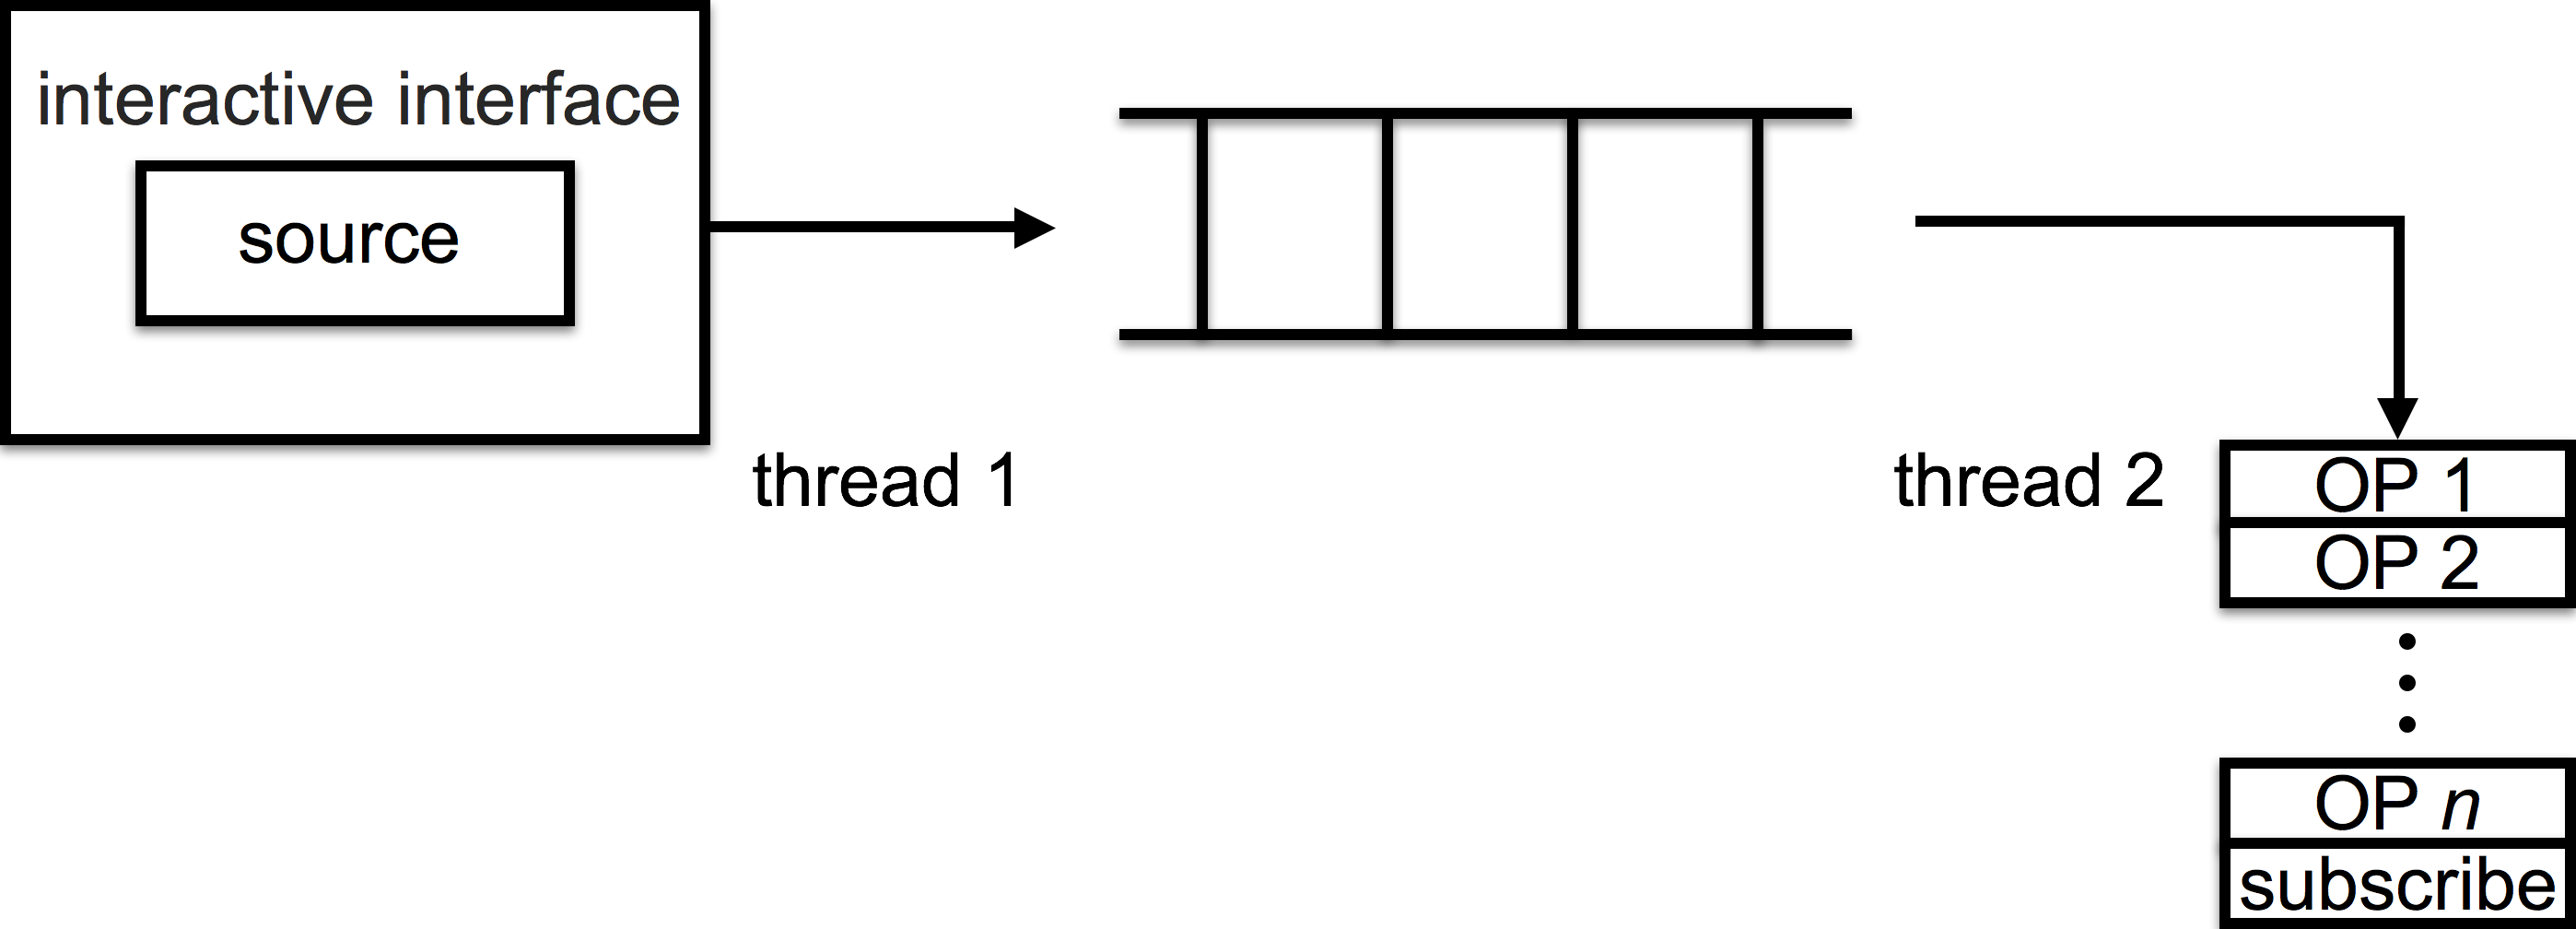
\includegraphics[width=0.63\textwidth]{figures/Approach.png}
	\end{center}
	\caption{Schematic representation of our approach}
	\label{fig:new-approach}
\end{figure}

With this approach we have reduced the problem of overproduction to a problem of controlling the size of a buffer to be as small as possible, without the buffer being exhausted by a fast consuming downstream. A buffer size that is too small can lead to a needless delay in consuming the data, whereas a too large buffer size is not desirable as well, given that we want to spend as little resources as possible. The complicating factor here is that it is unknown at all times how long it will take for the source to produce a next element.

In order to overcome this unknown factor, control the size of the buffer and only request new elements from the source when needed, we will use a well-known technique from mechanical and electrical engineering called \textit{feedback control}. Since this is a technique that is unfortunately not as well-known in computer science and software engineering as it is in other parts of science and engineering, we will introduce this technique in the upcoming chapters, develop an API to work with this technique in general and present the rest of our solution to the overproduction problem after that.

Obviously RxJava in its current stage cannot be used to implement this solution, as it already has a backpressure implementation. Therefore we will use the RxMobile \cite{RxMobile} reference implementation which was recently written in Scala by Erik Meijer as a basic API for reactive programming and build our approach on top of that without the need of rewriting any existing code.


\clearpage
\chapter{Introduction to feedback control}
Control is something we deal with on a daily basis. Whether it is the temperature in our houses, the number of people in line at the supermarket's checkout or something more critical like the number of neutrons emitted during a nuclear reaction in a reactor, we have to control it to avoid potential chaos.

In software development we too want to have control over the products we both create and use. For example, most applications have a settings menu where the user can alter the application's behavior to their liking; to ensure our code to be working correctly we use compilers, IDEs and automated testing tools that help us trace errors and bugs; companies like Google, Facebook and Twitter do A/B-testing and other kinds of user studies when introducing new features and with that control and improve the usability of their product; and last but not least, in cloud computing we want to control the number jobs in a queue and scale up or down depending on the amount of jobs in the queue, such that all jobs get executed as fast as possible with spending the least amount of resources.

A common factor in controlling a system is the notion of feedback: you change something in the environment and see how well it adjusts towards your desired outcome. If the lines at checkout get too long, most likely an extra cash register needs to be opened; if your users don't perform well on an A/B-test of your latest features, you should probably revise these features rather than bringing them into production; and when you alter the settings in an application, you check whether the new behavior is more to your desire and maybe fiddle around with them some more until it is more to your liking.

Controlling a system without the notion of feedback is possible, however this requires an exact model of the system under control. External forces that are not part of the model cannot be allowed to disturb the system. In most cases this model does unfortunately not exist and control has to incorporate the system's output to come up with it's next input. If the output is not taken into account, the system can drift off and end up in undesired situations. A nice example of this are Microsoft's user studies: the user's feedback was not taken into account when Office 2007 introduced the ``ribbon'' to replace the existing user interface nor when the start button disappeared in Windows 8 and suddenly every Windows user lost their 20+ years of accumulated muscle memory for commanding the Windows operating system \cite{meijer2014-embracing-the-hacker-way}.

In physics and engineering, feedback control is a commonly used technique and is also fully backed by mathematics. A series of equations and theorems such as Laplace Transforms and differential equations describe the abstract behavior of a feedback controlled system and allow to evaluate its outcome after running it for a certain time and with a certain input \cite{hellerstein2004-feedback, janert2013-feedback}. These theorems and equations are usable in science because everything else is described in the `language of mathematics' as well. We have known the differential equations to Newton's law of cooling, damped harmonic oscillators and so forth for centuries, as well as their Laplace Transforms, which are needed for the `feedback equations'.

This is all in contrast to the current situation in computer science. Although proven to be very effective in physics, computer science has not yet widely adopted the techniques of feedback control. Instead, complex algorithms are written to control a web cache or do cloud scaling. Although it seems very naturally applicable, it is surprising to find that such a simple and effective technique is mostly ignored.

A potential reason for this lack of using feedback control lies in the fact that computer science does not yet fully understand the whole mathematical background of the datastructures and applications that are being used and created. Given this lack of understanding, we are not yet able to describe to which laws our datastructures and application obey. What would be the equivalent of Newton's laws for a web cache \cite{janert2013-feedback}? Only recently some work has been done on understanding the mathematics behind this \cite{beckmann2015-cache-calculus} and we may very well see more of this in the future, which will eventually enable computer science to create a more formal mathematical model with theorems and equations equivalent to physics.

The lack of applying feedback control in computer science is also reflected in this technique commonly not being taught in university degree computer science education. Although it is one of the standard courses in physics and engineering studies, it is not at all present in the computer science curricula. And in the rare occasions it is taught, it is done in a way that a physics student would learn about it, namely as yet another maths course, even though this way of treating feedback control in computer science is not really applicable!

In this chapter we will introduce the basic concepts of feedback control with as little mathematics as possible. We will start with an overview of what a feedback system consists of and how it works. Next we will go into some detail on how to control a feedback system. Finally we will introduce a simple toy example that demonstrates the power of feedback control and translates these concepts into an imperative style program.

\section{Overview}
In general a system is controlled by feedback when its next input value is (partially) determined by its previous output(s). The reason for taking the previous output into account while coming up with a next input is due to external forces that may impacting the system in unexpected ways. These external forces do not come regularly, are not predictable and are also not equally strong each time, hence a notion of uncertainty in the system's behavior occurs. Due to this uncertainty, a model that accurately calculates the system's next input either does not exist or would be too complex. The solution for incorporating the uncertainty from external forces is to use a feedback cycle around the system: the system's output (affected by both the system's input and any external forces) is measured and compared to a desired reference value, after which their difference is transformed into the system's next input.

Important to mention here early on is that controlling a system with a feedback cycle is not a solution to optimization problems. Tasks like ``\textit{Make the flow through the system as large as possible}'' cannot be accomplished with feedback loops \cite{janert2013-feedback}, as they compare the system's current output with a known reference value. Tasks like this require some kind of optimization strategy that determines the reference value, after which a feedback loop can be used to bring and keep the system's output in this desired state.

The input and output of a feedback controlled system are not to be confused with the actual input and output of this system. The air conditioning or heating system has an actual output of hot or cool air, whereas the feedback system's output can be any other measurable metric such as the new temperature after the actual output is applied or the temperature difference caused by the actual output. The input and output of a feedback controlled system are often referred to \textit{control input} and \textit{control output}.

\subsection{Calculating the next control input}
Every time the control output produces a new value, it is compared to a reference value or \textit{setpoint} for it to calculate the \textit{tracking error} as the deviation of the control output from the setpoint:

\begin{equation} \label{eq:tracking-error}
\text{tracking error} = \text{setpoint} - \text{control output}
\end{equation}

This tracking error is then transformed into the next control input by the \textit{controller}. When the tracking error is positive (thus the control output is less than the setpoint), the controller has to produce a new control input that ultimately raises the control output to the same level as the setpoint, such that the tracking error becomes zero. Of course this depends on the \textit{directionality} of the system: for some systems the control input needs to be lowered for the system output to be raised. The controller must be able to make this distinction and therefore has to know the directionality of the system. For example, a heating system requires the controller to \emph{raise} the control input to get a higher temperature, whereas a cooling system requires the controller to \emph{lower} the control input to get a higher temperature.

Besides the directionality, the controller also needs to decide on the magnitude of the correction. If the magnitude is too high, the controller could overcompensate and turn a positive tracking error into a negative tracking error and vice versa, causing the system to oscillate between two states. The worst situation occurs when the negative tracking error caused by the overcompensation of the positive tracking error is larger than the positive tracking error: this results in an ever growing amplitude of the oscillation, which eventually makes the whole system unstable and in the end causes it to blow up.

On the other hand, the magnitude can be too low, causing the controller to undercompensate. This causes tracking errors to persist for a longer time than necessary and makes the system respond slow to disturbances. Although this is less dangerous than instability, this slow behavior is unsatisfactory as well.

In general we require the controller to take in a tracking error and come up with a new control input such that the tracking error will go to zero as soon as possible. For this it turns out that the controller does not need to know anything about the controlled system, but only requires information about the directionality of the system and the magnitude of the correction.

\subsection{Architectural overview}
The architecture of a feedback system is usually depicted as a set of boxes connected with arrows. This way we get a quick overview of the design without worrying about the exact implementation of the various components. The general architecture of a feedback system as discussed above is shown in \autoref{fig:feedbackArchitecture}. Notice that here the control output is negated on the way back and is then added to the setpoint in order to calculate the tracking error. This is common practice as some more preprocessing is required before comparing the control output with the setpoint. For example, the output may contain noise which needs to be smoothened by some kind of filter. Of course preprocessing steps will also be drawn in this overview if applicable.

\begin{figure}[H]
	\begin{center}
		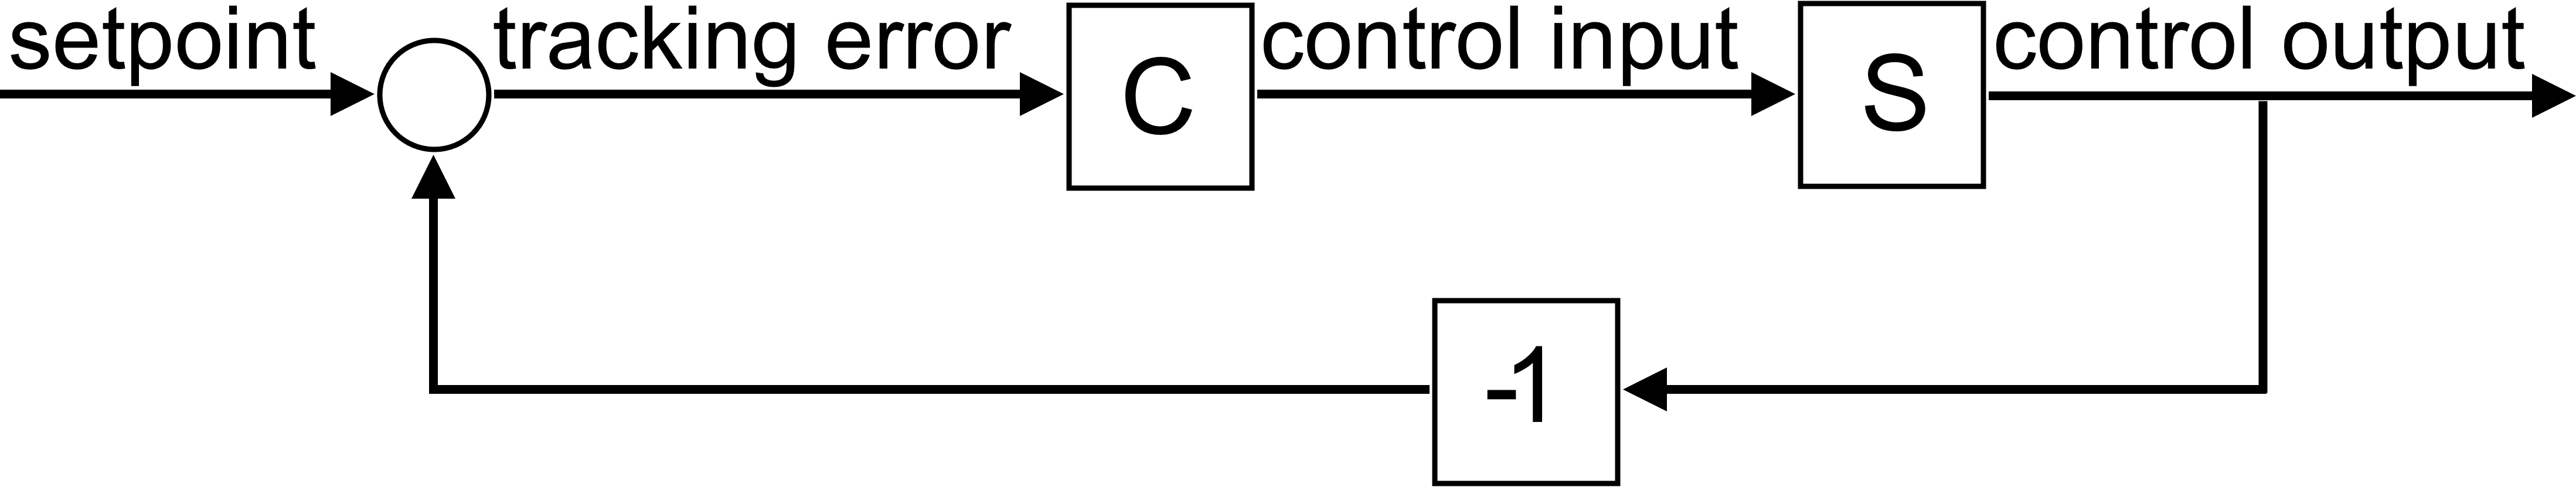
\includegraphics[width=0.85\textwidth]{figures/FeedbackBig.png}
	\end{center}
	\caption{The architecture of a feedback control system}
	\label{fig:feedbackArchitecture}
\end{figure}

Besides these filters, a controller may consist of multiple components by itself. When using an incremental controller, only the difference in the control input is outputted. For the actual input we need to maintain a running sum of all the previous controller outputs and in that way calculate the actual control inputs. Usually these extra steps are also depicted in the architectural overview as extra boxes and arrows.


\section{Different types of controllers}
The control input in a feedback system is the value that tells the system under control to behave slightly different than it did and possibly incorporating external disturbances on the system in a better way. As discussed in the previous section, this control input value is computed in the controller part of the feedback system. Although one might expect differently, the controller itself does not turn out to be very smart or know a whole lot about the system under control. As mentioned before, a controller in fact only needs to know about directionality of the system and the magnitude of the correction for it to work just fine. There are a number of controllers that only need these two pieces of information and that are commonly used in physics, mechanics and electronics.

\subsection{On/Off control}
The most simple controller one can think of is just an on/off switch. Whenever the tracking error is positive, the controlled system is turned on and when the tracking error becomes negative it is turned off again\footnote{Of course this is dependent upon the directionality of the system under control.}. For simple systems this kind of control will suffice, although it will not be a very effective approach.

An application of this kind of control might be a air conditioning system that turns on when the temperature exceeds a preset level. In this example the control output is the current temperature in the room, the setpoint is the preset temperature, the control input is a boolean value which determines whether the system should be on of off and the directionality of the system is negated. Imagine the temperature initially being much too high, causing the air conditioning to turn on right away. After a certain amount of time the temperature reaches the desired setpoint (the tracking error becomes zero), hence the system will shut down. Shortly after the air conditioning system is shut down, the temperature starts increasing again. This immediately causes a deviation from the setpoint, forcing the air conditioning to turn on again. Soon enough the temperature is low enough again for the system to be turned off, after which the cycle starts all over again. Of course this kind of behavior is very annoying to everyone working in this room, as the air conditioning continuously turns off and on again. Besides that, this behavior costs an unnecessary amount of energy for turning the system on and off, which is not really desirable either.

Obviously this behavior is caused by the controller that dictates to turn off the system whenever the setpoint is met. Due to external disturbances such as whether conditions the feedback system is off track soon again, which causes the controller to decide to turn the controlled system back on.

Small improvements that are often used in these kinds of systems are introducing a dead zone or Schmitt trigger, which causes the system to continue with the same corrective action until a certain threshold or a certain amount of time is exceeded. This prevents the controller from overreacting on sudden and short spikes in the control output. In the case of the air conditioning an addition such as this will cause the controller to not immediately send a `turn off signal' when the setpoint is zero and will not activate the system with the slightest deviation, but instead waits a little longer until a threshold is exceeded before activating or deactivating the system again.

\subsection{Proportional control}
Another simple controller 


\section{An extended example}
To get a better feel for how a feedback control system works in practice, we will discuss a simple but interesting application of feedback control that uses the theory covered in the previous sections. In this section we show an imperative reference implementation. In the next chapter we will continue to use and refactor this application as we come up with an API for constructing and executing feedback systems. The application at hand is a port from the original implementation by Nikita Leshenko in Javascript, CSS and HTML \cite{nikital-balltracker}. We will however use Scala as our programming language and JavaFx for drawing the graphics on the screen. To get a feel of what this application is doing we strongly recommend to have a look at the online version\footnote{\url{http://nikital.github.io/pid/}} first before proceeding with this section!

The application consists of a flat surface on which a ball can move around. The goal is to move the ball from its initial position to the position on the surface that the user clicks on with the mouse. \Cref{fig:balltracker-initial} shows the ball in its initial state when the application starts. When the user clicks on the screen, the ball starts moving to that position as shown by \Cref{fig:balltracker-moving}. Besides the background and the ball, also the desired position, a dashed line between the ball and the desired position, the acceleration in both the $x$ and $y$ directions and a trail of previous positions are drawn (which are fading away over time). After some time the ball is at its desired position and waits there for a new position to navigate to (\Cref{fig:balltracker-reached}). Notice that the desired position can also be updated while the ball is still moving, in which case it moves to the new and discards the old destination.

\begin{figure}
	\centering
	\begin{subfigure}[b]{0.80\linewidth}
		
\includegraphics[trim = 0mm 110mm 0mm 0mm, clip, width=\linewidth]{figures/BallTracker-initial.png}
		\caption{Initial}
		\label{fig:balltracker-initial}
	\end{subfigure}
	
	\begin{subfigure}[b]{0.80\linewidth}
		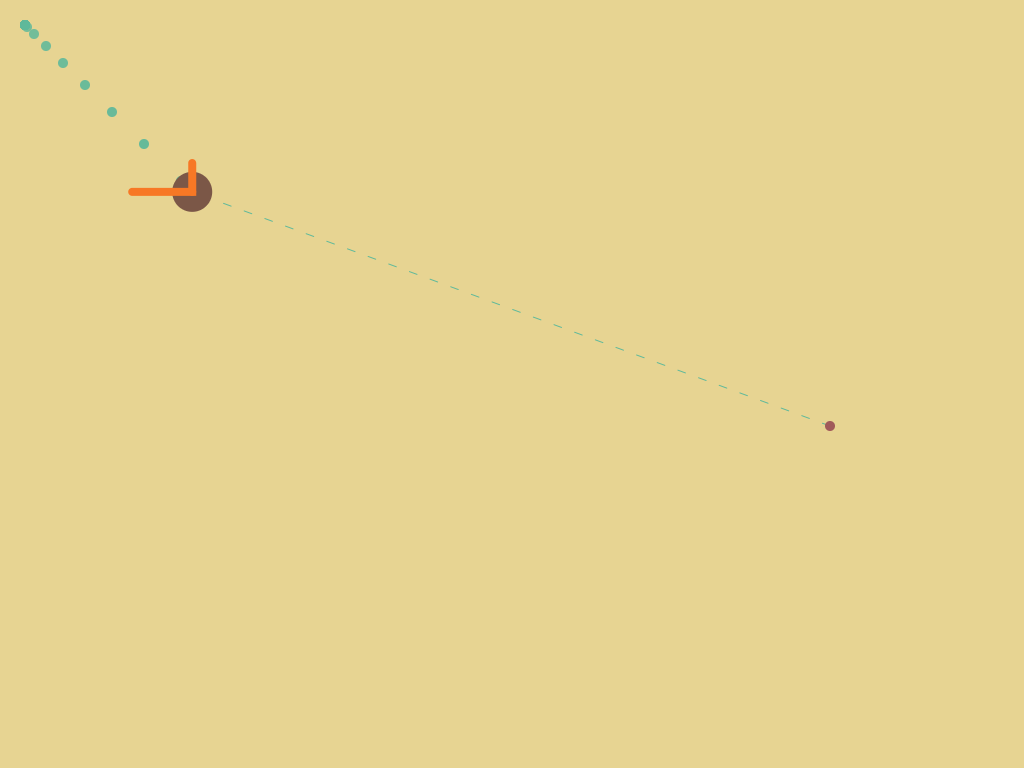
\includegraphics[trim = 0mm 110mm 0mm 0mm, clip, width=\linewidth]{figures/BallTracker-moving.png}
		\caption{Moving to desired position}
		\label{fig:balltracker-moving}
	\end{subfigure}
	
	\begin{subfigure}[b]{0.80\linewidth}
		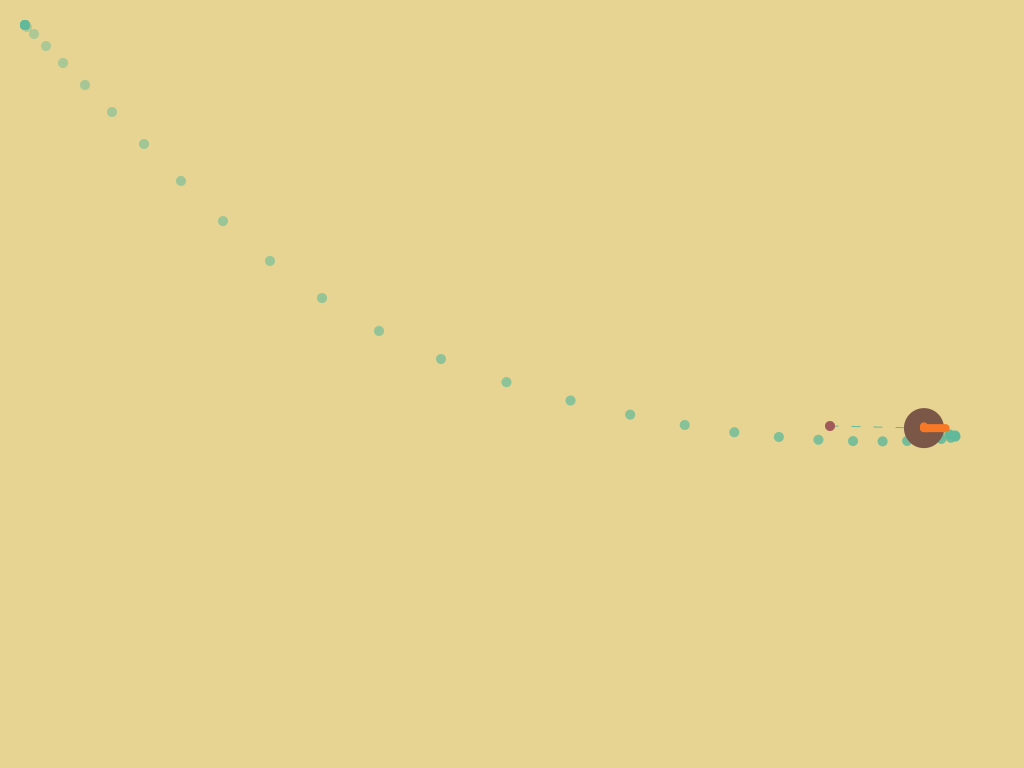
\includegraphics[trim = 0mm 110mm 0mm 0mm, clip, width=\linewidth]{figures/BallTracker-overshooting.png}
		\caption{Moving to desired position, overshooting a bit}
		\label{fig:balltracker-moving}
	\end{subfigure}
	
	\begin{subfigure}[b]{0.80\linewidth}
		
\includegraphics[trim = 0mm 110mm 0mm 0mm, clip, width=\linewidth]{figures/BallTracker-desired.png}
		\caption{Reached desired position}
		\label{fig:balltracker-reached}
	\end{subfigure}
	\caption{Ball tracker}
	\label{fig:balltracker}
\end{figure}

In order to allow the ball to move in a natural way, we remind the reader of some basic equations from physics that describe the one dimensional motion of an object as a function of time (\Cref{eq:motion}). Here $x_t$, $v_t$ and $a_t$ are the ball's position, velocity and acceleration at time $t$ respectively. For two-dimensional motion we can combine two sets of these equations for both dimensions.

\begin{subequations}
	\begin{equation}
		x_t = x_{t - 1} + v_t \cdot \Delta t
	\end{equation}
	\begin{equation}
		v_t = v_{t - 1} + a_t \cdot \Delta t
	\end{equation}
	\label{eq:motion}
\end{subequations}

The implementation of these required pieces of physics can be found in \Cref{lst:ball-physics}. We first define a \code{Position}, \code{Velocity} and \code{Acceleration} as tuples of \code{Double} as well as some mathematical operations on the tuple type. The \code{Ball} class describes the state of the ball having a position, velocity and acceleration. A second constructor (\code{apply}) defines the initial position with no acceleration or velocity. The method \code{accelerate} on this class takes a new acceleration and calculates a new state for the ball according to \Cref{eq:motion}. Notice that we discard the $\Delta t$ term, since this will always be equal to 1. To keep track of the ball's previous positions we define \code{History} to be a queue of \code{Position}s.

\begin{minipage}{\linewidth}
\begin{lstlisting}[style=ScalaStyle, caption={Ball motion physics}, label={lst:ball-physics}]
type Position $=$ (Double, Double)
type Velocity $=$ (Double, Double)
type Acceleration $=$ (Double, Double)
type History $=$ mutable.Queue[Position]

implicit class Tuple2Math[X: Numeric, Y: Numeric](val src: (X, Y)) {
  import Numeric.Implicits._
  def +(other: (X, Y)) $=$ (src._1 + other._1, src._2 + other._2)
  def -(other: (X, Y)) $=$ (src._1 - other._1, src._2 - other._2)
  def *(scalar: X)(implicit ev: Y $=:=$ X) $=$ (scalar * src._1, scalar * src._2)
  def map[Z](f: X $\Rightarrow$ Z)(implicit ev: Y $=:=$ X): (Z, Z) $=$ (f(src._1), f(src._2))
}

case class Ball(acc: Acceleration, vel: Velocity, pos: Position) {
  def accelerate(nAcc: Acceleration) $=$ Ball(nAcc, vel + nAcc, pos + vel + nAcc) |\label{line:accelerate}|
}
object Ball {
  def apply(radius: Double) $=$ Ball((0.0, 0.0), (0.0, 0.0), (radius, radius))
}
\end{lstlisting}
\end{minipage}

The next step in creating this application is to design the feedback system itself (\Cref{fig:balltracker-diagram}). The \textit{system under control} here is of course the ball, from which at any point acceleration, velocity and position can be measured. Given that our \textit{setpoint} is equivalent to the position of where the ball should end up eventually, it makes most sense to define the \textit{control output} as the current position of the ball. From this it follows that the \textit{tracking error} represents the distance to be traveled before reaching the desired position. Depending on the distance, a controller can then decide how much it wants to speed up the ball by providing a new acceleration as the system's \textit{control input}. To get the ball's next position, this acceleration has to be integrated twice to get the ball's position after $\Delta t$ time.

To transform a distance into an acceleration, we can use the power of the PID controller. As discussed before this controller is renowned for its effectiveness and simplicity and is therefore most commonly used in all kinds of feedback systems, especially those who deal with floating point control inputs and outputs. For this use case it makes absolute sense to use this controller as well. The \textit{proportional controller} will look at the current distance to be traveled and comes up with some amount of acceleration. However, this acceleration will approach zero as the ball approaches its destination, causing it to keep its same velocity rather than slowing down. To prevent this, we need a strong \textit{derivative controller} that can counteract this velocity and slow down the ball as the distance is becoming smaller. For the purpose of looking back at previous distances we also add an \textit{integral controller} into the mix.

\begin{figure}[H]
	\begin{center}
		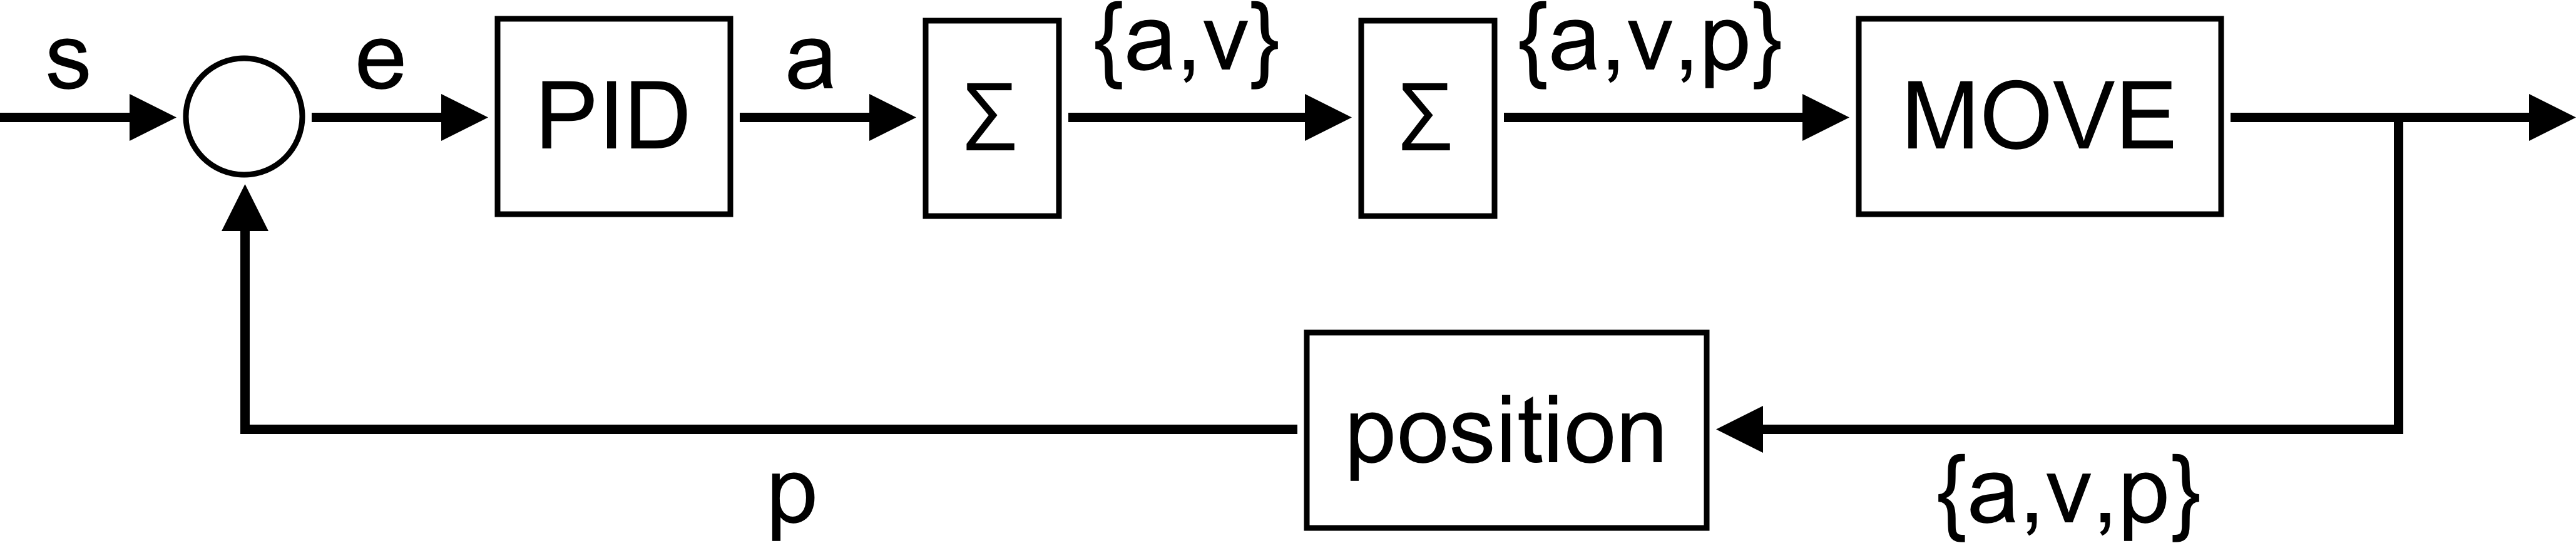
\includegraphics[width=0.85\textwidth]{figures/BallTracker-diagram.png}
	\end{center}
	\caption{Architecture of the ball movement control system}
	\label{fig:balltracker-diagram}
\end{figure}

Both the PID controller and the feedback system are implemented in \Cref{lst:ball-feedback}. After some initialization we define an iteration of the controller following \Cref{eq:proportional-control,eq:integral-control-discrete,eq:derivative-control} in the \code{pid} function on \cref{line:pid-function}. Again notice that this operates on the tuple types and uses the operators defined in \Cref{lst:ball-physics}. This function returns a new \code{Acceleration} which corresponds to the control input as described above.

The PID controller is then used in the construction of the feedback cycle (\cref{line:update}). It is first scaled down in such a way that it has an absolute maximum acceleration $0.2$, after which it is fed into the controlled system. This calls the \code{accelerate} function on the \code{Ball} (\Cref{lst:ball-physics} \cref{line:accelerate}), which calculates the ball's new velocity and position. The new state is then stored in the \code{ball} variable, which represents the latest control output. The rest of this function deals with managing the history and redrawing the application, which are considered not relevant for the implementation of the feedback system itself. The omitted code can be found in \Cref{app:ball-movement}.

Now that the feedback cycle is implemented, we can plug this in a JavaFx application that contains the canvas on which the application is drawn, as well as assigning the setpoint value and looping through the feedback cycle every 16 milliseconds. The code for this can be found in \Cref{app:ball-movement} as well.

Notice that with this feedback system we lack the notion of an external disturbance on the system under control. In this case there is none since the system is just the two \textit{sigma}s and the \textit{DRAW}. One could argue that the changing setpoint is kind of a disturbance, although this is by definition not the case. An example of an external disturbance on this particular system could be the terrain not being flat but rather containing hills and valleys. This would influence the ball's movement because of gravity, which would add a force in a third direction. For the sake of simplicity of this example we decided to not add this feature and stick with the flat terrain. We leave implementing this feature as an exercise to the reader.

\begin{minipage}{\linewidth}
\begin{lstlisting}[style=ScalaStyle, caption={Ball drawing}, label={lst:ball-feedback}]
var ball $=$ Ball(ballRadius)
var setpoint $=$ ball.position
var prevError, integral $=$ (0.0, 0.0)

// initializing history
// ...

def pid: Acceleration $=$ { |\label{line:pid-function}|
  val (kp, ki, kd) $=$ (3.0, 0.0001, 80.0)
  val error $=$ setpoint - ball.position
  val derivative $=$ error - prevError

  integral $=$ integral + error
  prevError $=$ error

  (error * kp + integral * ki + derivative * kd) * 0.001
}

def update(implicit gc: GraphicsContext): Unit $=$ { |\label{line:update}|
  val acceleration $=$ pid map (a $\Rightarrow$ math.max(math.min(a, 0.2), -0.2))
  ball $=$ ball accelerate acceleration

  // managing the history
  // ...

  // drawing all the elements
  // ...
}
\end{lstlisting}
\end{minipage}

\subsection*{PID control tuning}
As one can see from the code, there is not much room in the feedback system to work on the performance or accuracy of the ball movement control. The controlled system, in \Cref{fig:balltracker-diagram} consisting of the two \textit{sigma}s and the \textit{DRAW}, is fixed by the equations in \ref{eq:motion}. Also the \textit{position} block is not something that can improve the performance and accuracy. The only place to do so are the three controller gains in the PID controller function. In \Cref{lst:ball-feedback} \cref{line:pid-function} we set these values to $k_p = 3.0$, $k_i = 0.0001$ and $k_d = 80.0$\footnote{We will refer to these values as \textit{default values}.}. These values originate from the original version of this application by Nikita Leshenko \cite{nikital-balltracker}. In his implementation one can also alter these values and see how they affect the performance and accuracy of the ball movement.

In this section we will discuss some effects of the controller gains by altering the default values and observing how they alter the behavior of the ball's movement. For this we scale down the original application to 1 dimension, initialize the ball at position 20 (the ball is 20 units wide on the screen) and set the ball's setpoint at position 500. We let the ball move from its original position to the setpoint and meanwhile record the proportional, integral and derivative controller that make up the PID controller as well as the total acceleration\footnote{This is the acceleration before multiplying it with $0.001$ and maximizing it at $0.2$} and the balls position after applying the newest acceleration. We then plot these results, where the horizontal axis represents time, the primary vertical axis represents the accelerations and the secondary vertical axis represents the ball's position. The default behavior of the application is shown in \Cref{fig:balltracker-pid-default}.

We already discussed the setting of only having a proportional gain (set $k_i$ and $k_d$ to zero): as the ball approaches its destination, its acceleration will approach zero, meaning that the ball will not slow down but will rather keep moving with the same velocity. The exact behavior can be seen in \Cref{fig:balltracker-pid-kp-only}.The acceleration becomes zero as the ball reaches its setpoint, but only slows down past this point. At the time the ball comes to a hold, the distance with the setpoint is thus large that it needs to accelerate again (in the other direction). This process will repeat itself indefinitely without ever coming to a halt at the setpoint.

\begin{figure}
	\centering
	\begin{subfigure}[b]{0.49\linewidth}
		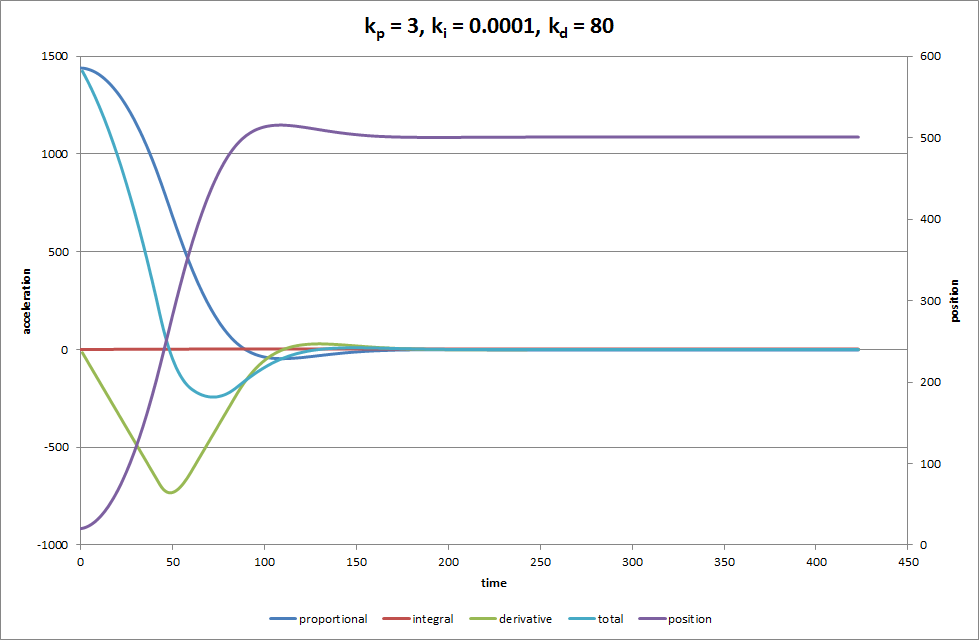
\includegraphics[width=\linewidth]{{figures/balltracker-pid/kp=3,ki=0.0001,kd=80}.png}
		\caption{$k_p = 3$, $k_i = 0.0001$, $k_d = 80$ (default)}
		\label{fig:balltracker-pid-default}
	\end{subfigure}
	\begin{subfigure}[b]{0.49\linewidth}
		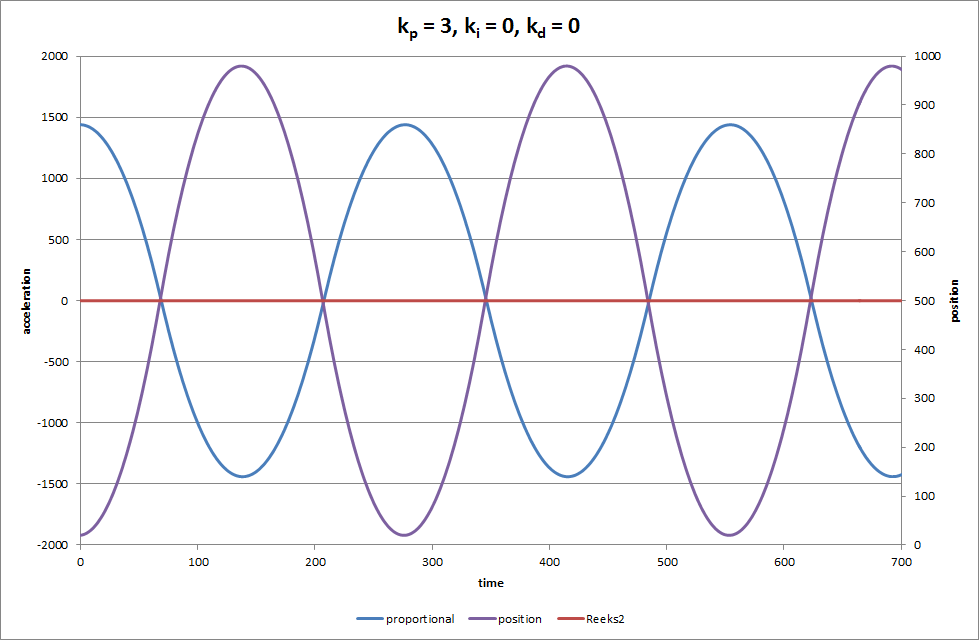
\includegraphics[width=\linewidth]{{figures/balltracker-pid/kp=3,ki=0,kd=0}.png}
		\caption{$k_p = 3$, $k_i = 0$, $k_d = 0$}
		\label{fig:balltracker-pid-kp-only}
	\end{subfigure}
	
	\begin{subfigure}[b]{0.49\linewidth}
		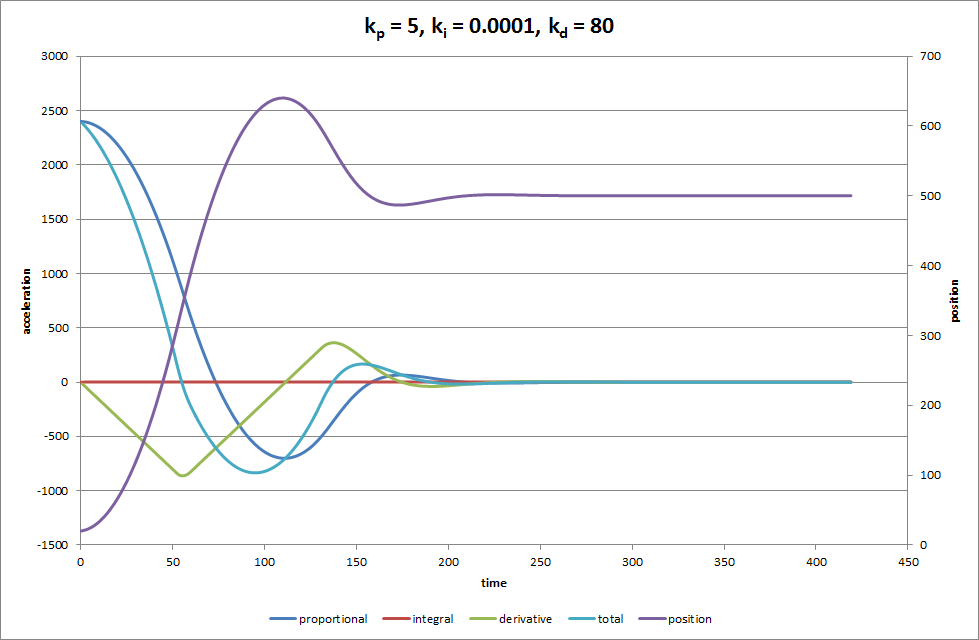
\includegraphics[width=\linewidth]{{figures/balltracker-pid/kp=5,ki=0.0001,kd=80}.png}
		\caption{$k_p = 5$, $k_i = 0.0001$, $k_d = 80$}
		\label{fig:balltracker-pid-kp-higher}
	\end{subfigure}
	\begin{subfigure}[b]{0.49\linewidth}
		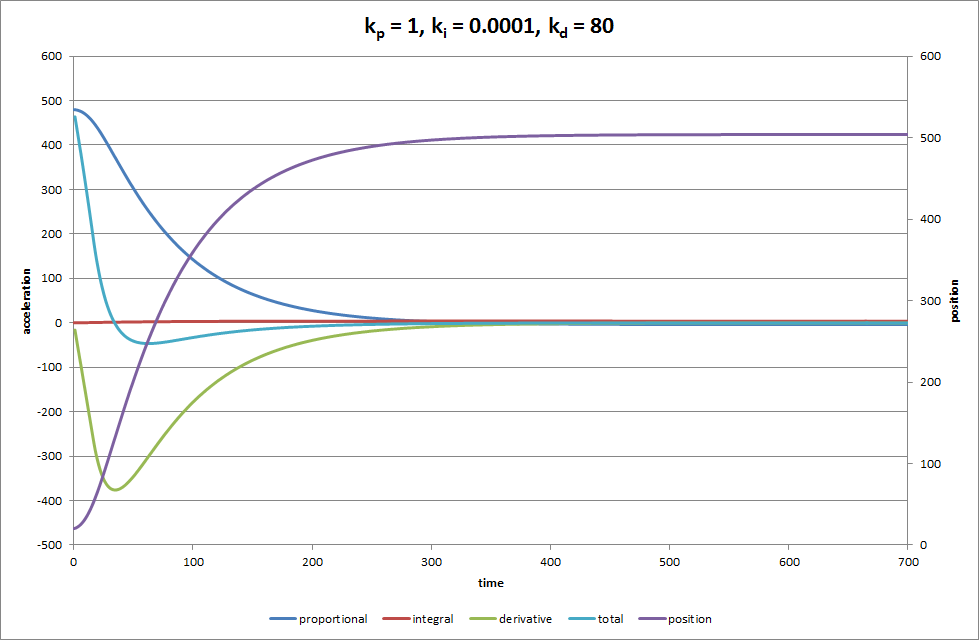
\includegraphics[width=\linewidth]{{figures/balltracker-pid/kp=1,ki=0.0001,kd=80}.png}
		\caption{$k_p = 1$, $k_i = 0.0001$, $k_d = 80$}
		\label{fig:balltracker-pid-kp-lower}
	\end{subfigure}
	
	\begin{subfigure}[b]{0.49\linewidth}
		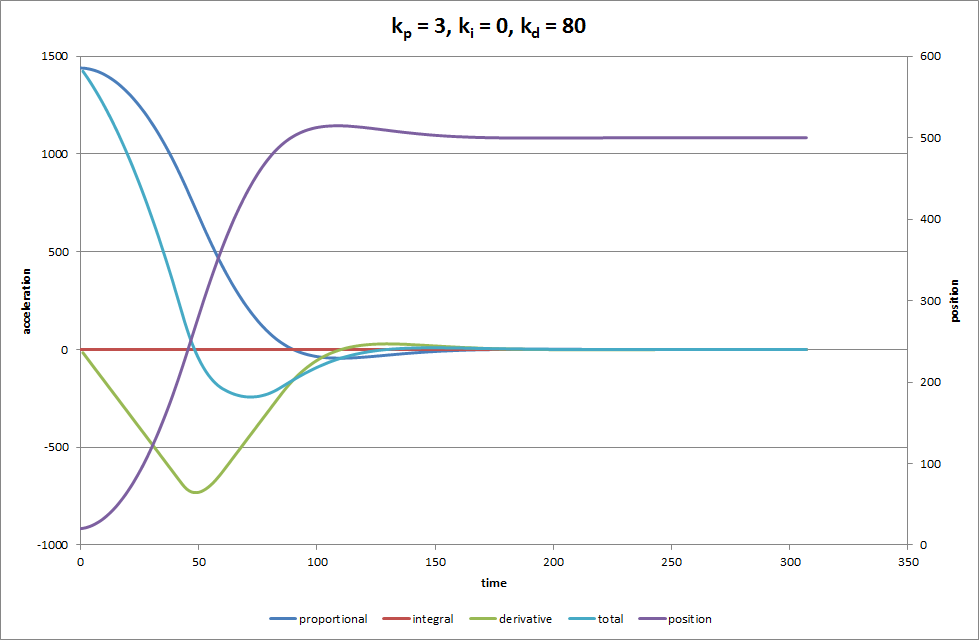
\includegraphics[width=\linewidth]{{figures/balltracker-pid/kp=3,ki=0,kd=80}.png}
		\caption{$k_p = 3$, $k_i = 0$, $k_d = 80$}
		\label{fig:balltracker-pid-ki-zero}
	\end{subfigure}
	\begin{subfigure}[b]{0.49\linewidth}
		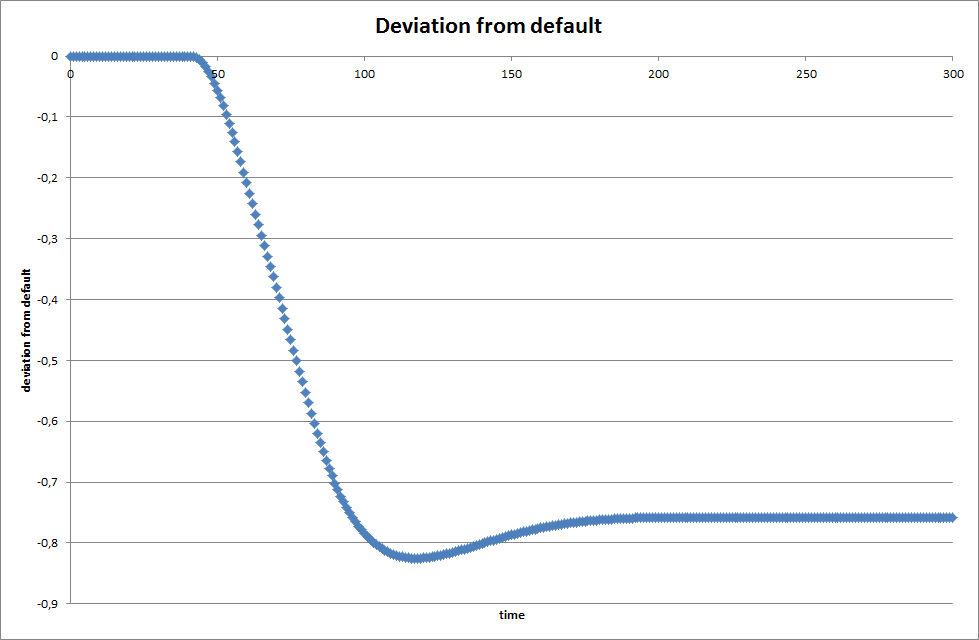
\includegraphics[width=\linewidth]{{figures/balltracker-pid/kp=3,ki=0,kd=80,diff}.png}
		\caption{$k_p = 3$, $k_i = 0$, $k_d = 80$}
		\label{fig:balltracker-pid-ki-zero-diff}
	\end{subfigure}
	
	\begin{subfigure}[b]{0.49\linewidth}
		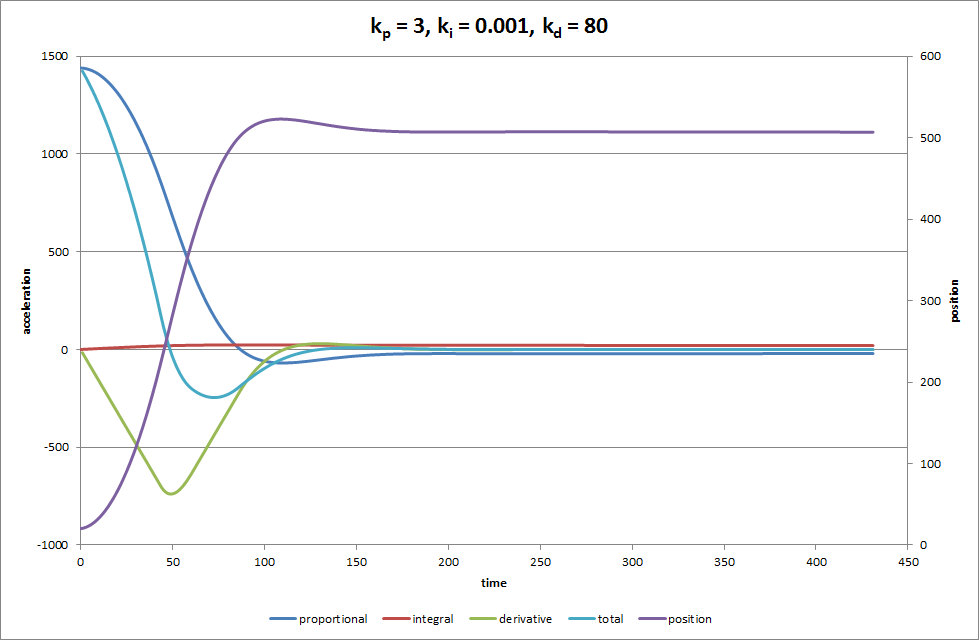
\includegraphics[width=\linewidth]{{figures/balltracker-pid/kp=3,ki=0.001,kd=80}.png}
		\caption{$k_p = 3$, $k_i = 0.001$, $k_d = 80$}
		\label{fig:balltracker-pid-ki-higher}
	\end{subfigure}
	\begin{subfigure}[b]{0.49\linewidth}
		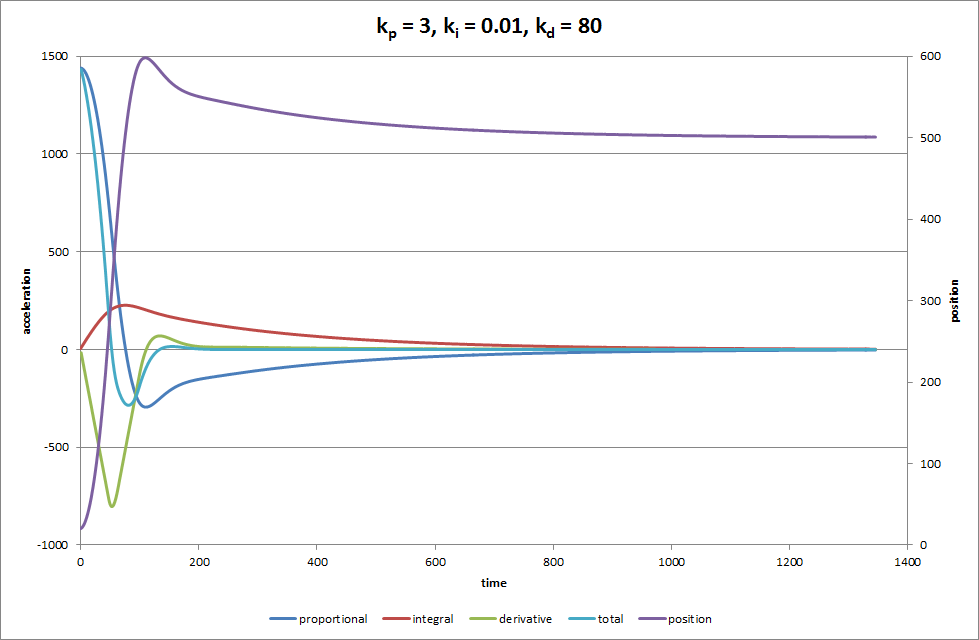
\includegraphics[width=\linewidth]{{figures/balltracker-pid/kp=3,ki=0.01,kd=80}.png}
		\caption{$k_p = 3$, $k_i = 0.01$, $k_d = 80$}
		\label{fig:balltracker-pid-ki-highest}
	\end{subfigure}
	\caption{Various values for the controller gains in a PID controller}
	\label{fig:pid-settings}
\end{figure}

On the other hand, altering the default settings with a larger value for proportional controller gain (for example $k_p = 5$) will cause the ball to overshoot its destination and have more oscillation around the destination before coming to a halt (\Cref{fig:balltracker-pid-kp-higher}). A smaller value ($k_p = 1$) will have the opposite effect (\Cref{fig:balltracker-pid-kp-lower}): it slows the ball down too early and also deviates a bit from the setpoint when it halts (position 503 where 500 was expected). This is expected and according to the theory as described earlier as well as by Janert \cite{janert2013-feedback}: a too high controller gain will cause overshooting the setpoint and oscillations, whereas a too low controller gain will cause undershooting and approaching the setpoint too slow.

The integral controller gain is set very low by default. This is no surprise, as the previous tracking errors (the distance still to be traveled) are not of much interest for the transformation to a new acceleration. As far as we were able to observe, discarding the integral factor complete does not really hurt the performance; in fact it only improves the accuracy (\Cref{fig:balltracker-pid-ki-zero,fig:balltracker-pid-ki-zero-diff}).

Increasing this value will however lead to some interesting behaviors. A value like $k_i = 0.001$ (10x higher than default) will cause the ball to end up slightly offset of its actual destination (\Cref{fig:balltracker-pid-ki-higher}). A value like $k_i = 0.01$ (100x the default value) has an even more peculiar behavior as it first approaches the destination in somewhat normal fashion, then almost stops at an offset position and creeps forward very slowly to the actual destination and holds at the correct position. This of course has to do with the relative weight of the integral part of the controller with regards to the weight of the proportional and derivative parts.

The derivative controller gain has the largest relative impact on the PID controller with its default value being set to $k_d = 80$. This value determines most of the oscillation in the system: the larger this value is, the less oscillation occurs. On the other hand, having a derivative controller gain that is too big is not good either as it will slow down the ball too early and make it creep towards its destination.

Tuning a PID controller is mainly a process of trial and error. One needs to find an optimal set of three values for the controller gains and with that has a very limited number of parameters to tune. For applications in physics there exist equations that give accurate values for these three parameters, although these only work correctly if the behavior of the system under control is fully known and can be translated in differential equations\footnote{Technically this could have been done for this example since it comes straight from physics, but for the sake of demonstrating it in the context of computer science we choose not to do so.}.

Janert spends a couple of chapters on the topic of controller tuning in de context of computer science \cite{janert2013-feedback} and goes into much detail to come up with equations that can give a first idea of the range in which to search for the optimal controller gains. This however are just an indication and still require experimentation to come up with the best solutions.



\clearpage
\chapter{An API for feedback control}

While studying the principles of feedback control, we discovered that there are hardly any publicly available libraries or APIs that abstract over the notions of feedback control, allowing us to create and execute feedback systems, both in simulation and in practice. Although surprising at first, this is completely in accordance with the earlier observation that feedback control is not (yet) a commonly used technique in computer science\footnote{Even though we were not able to find existing APIs for this purpose, we would not be surprised if companies turned out to have libraries like this in private.}. Surely, we can write the code ourselves as shown in \Cref{sec:imperative-balltracker}, but that isn't really reusable, creates the danger of copy-paste behavior and is more prone to bugs than a dedicated API.

In this chapter we present our own API for creating and executing feedback systems that can potentially be used in production software. \todo{rest of the introduction and layout of this chapter}

\section{Related work}
One of the few libraries we found is described by Philip Janert in his book ``\textit{Feedback Control for Computer Systems}'' \cite{janert2013-feedback}. Janert presents a small framework for simulating feedback loops with the purpose of being a teaching tool that makes it simple and transparent to demonstrate the algorithms presented in several case studies and to encourage experimentation. He explicitly states that little emphasis was placed on elegant implementations or time efficiency and that this framework is not meant to be used in production software. What distinguishes his framework from other simulation frameworks for control systems (for example MatLab \cite{Matlab-Feedback}), however, is the way that the components that make up a feedback loop are implemented. As discussed before, most feedback systems in physics and engineering are described in terms of complex mathematics, using transfer functions and Laplace transformations, that operate in the frequency domain. Janert's API, however, allows algorithms to be implemented in the time domain, which is a more natural representation to software developers and people that are not familiar to the mathematics based approach.

One of the central aspects of Janert's framework is the \code{Component} class which contains two methods with the following signatures: \code{def work(u: Double): Double}, which encapsulates the dynamic function of a component, called once every feedback cycle and \code{def monitoring: String}, which is just a convenience function and allows for a uniform approach to logging. All components (controlled systems, controllers and more advanced building blocks like actuators and filters) are just subclasses of \code{Component} that implement these two methods. The feedback system is then simulated using a loop that iterates over time stamps and which calls the \code{work} method on the next \code{Component} with the result of calling the \code{work} method of the previous \code{Component}. Finally at the end of each loop cycle the result is printed to the console using the \code{monitor} method of the \code{Component} that represents the system under control.

As pointed out by Janert, this framework does well for simulation but is not really useful for production software. One concern with this framework is that it performs a feedback cycle with regular intervals between each other. However, one can easily imagine a controlled system which produces a control output very irregularly. In that case the feedback cycle has to respond to the emission of a new data point rather than asking the controlled system for its next input. Another concern related to this is the ability to handle concurrency appropriately. A component in the feedback loop might perform some kind of timing related work that requires running on a different thread or thread pool. Finally we should note that the subclasses of \code{Component} have to use mutable state if they want to store any data. Think of the Integral Controller, which has to store its current sum. Mutable state is something that computer science has come to terms with as not being so practical in some cases as we once thought it would be. Especially when introducing concurrency, mutable state is something you want to avoid at all cost!


\section{Towards a feedback API}
If we want to develop a library or API for feedback control we should keep a couple of things in mind. First of all the API should be production worthy: it should be able to drive production software/hardware and it should be easy for the developers of those systems to put together a feedback loop, without having to understand much about the mathematics that is going on in theoretical control theory. Also the concerns mentioned in the previous section should be kept in mind: the API should not rely on any form of mutable state if this is not desired by the developer, it should be easily able to support concurrency and asynchronicity and should not rely on any regularity in feedback cycles.

The idea by Janert to model a feedback system in the same way as it is drawn (see for example \Cref{fig:balltracker-diagram}) is something that looks very appealing to use as a foundation of our API. This means that we create a feedback system by composing smaller entities or by chaining transformations. In the same way for example Scala's collection API is build up, using (monadic) operators to transform and manipulate a collection. Likewise we will use higher order functions to compose feedback systems.

Some of the basic composition operations that are required for this to work are \textit{sequential composition}, which passes the output of the first component as the input of the second component, \textit{parallel composition}, which passes its input to multiple components and combines the output of each component into a single value using a combinator function, \textit{merging the output of two components} into a single value and \textit{feeding back the output of a component to its input} to create a circuit or feedback loop. Other composition operators that one can imagine are operators like the ones found in monadic APIs in Scala or Java 8 such as collections, \code{Future}, \code{Try}, \code{Option} or the Rx \obs. Examples of these are \code{map}, \code{filter}, \code{flatMap}, \code{take}, \code{drop}, \code{scan}, etcetera.

\subsection{Derivation}
\label{subsec:api-derivation}
To get to a suitable API we must first of all observe that a component can be thought of as a Mealy Machine \cite{mealy1955-mealymachine}. This is a special variant of the finite-state machine whose output values are determined by both its current input and its current state. It can mathematically be described as a 6-tuple $(\Sigma, \Gamma, S, s_0, \delta, \omega)$ \cite{carroll1989-theoryoffiniteautomata} where

\begin{itemize}
	\item $\Sigma$ denotes the input alphabet
	\item $\Gamma$ denotes the output alphabet
	\item $S$ denotes the finite nonempty set of states
	\item $s_0$ denotes the start (or initial) state; $s_0 \in S$
	\item $\delta$ denotes the state transition function; $\delta: S \times \Sigma \rightarrow S$
	\item $\omega$ denotes the output function; $S \times \Sigma \rightarrow \Gamma$
\end{itemize}

Note that the two functions $\delta$ and $\omega$ can be coalesced into a single function $\lambda: S \times \Sigma \rightarrow S \times \Gamma$.

This function $\lambda$ can also be written as a type definition in Scala:

\begin{lstlisting}[style=InlineScalaStyle]
type Component[S, I, O] $=$ (S, I) $\Rightarrow$ (S, O)
\end{lstlisting}

Notice that we use \code{I} and \code{O} to denote the input alphabet $\Sigma$ and output alphabet $\Gamma$ respectively. Equivalent to this type definition is the following static object \comp, containing a single function \code{apply}.

\begin{lstlisting}[style=InlineScalaStyle]
object Component {
  def apply[I, O, S](s: S, i: I): (S, O)
}
\end{lstlisting}

We can now rewrite \comp to be an interface and put the state \code{S} inside \comp implicitly. This removes the need for an input parameter of type \code{S} in the \code{apply} method, since the state is then contained inside the \code{this} pointer. Instead of the \code{S} in the return type we now, however, have to return a \comp that contains the output state.

\begin{lstlisting}[style=InlineScalaStyle]
trait Component[I, O] {
  // (im)mutable state in here
  def apply(i: I): (Component[I, O], O)
}
\end{lstlisting}

Instead of returning a tuple, the \code{apply} method can be split into two separate methods. \code{update} will accept something of input type \code{I} and return a new \comp, containing its new state. The output value of the transformation on the original component together with \code{I} can be retrieved from the newly returned \comp using the \code{action} method.

\begin{lstlisting}[style=InlineScalaStyle]
trait Component[I, O] {
  // (im)mutable state in here
  def update(i: I): Component[I, O]
  def action: O
}
\end{lstlisting}

This version of \comp gives us a first suitable implementation for composing over components. We will refer to this version as the \textit{Immutable Component}. Notice that this version is actually used in our blog post ``\textit{Feedback Control for Hackers}'' \cite{heest2015-feedback-for-hackers} as the basis of the simulation framework used in several case studies.

As an example of a component that inherits this interface, we will show an implementation of a component that maintains a running average of its input elements.

\begin{minipage}{\linewidth}
\begin{lstlisting}[style=ScalaStyle, caption={Implementation of \code{RunningAverage} using the \textit{Immutable Component} interface}, label={lst:immutable-runningaverage}]
class RunningAverage(n: Int, queue: Queue[Double])
      extends Component[Double, Double] {

  def update(u: Double): RunningAverage $=$ {
    if (queue.length $==$ n) queue.dequeue
    queue.enqueue(u)

    new RunningAverage(n, queue)
  }

  def action: Double $=$ queue.sum / queue.length
}
\end{lstlisting}
\end{minipage}

Here the internal state of the \comp, that was earlier referred to as \code{S}, consists of both the integer \code{n} (representing the number elements over which it has to calculate the running average), and the queue containing at most the latest \code{n} numbers that it received. Notice that \code{Component[Double, Double]} here specifies that the input type (the data type it can receive over which it calculates the average) and the output type (the data type of the average) are both \code{Double}. The \code{action} method is the one that calculates the actual average using the numbers that are present in the queue. On the other hand, receiving of the next value as well as keeping the queue up to date are done by the \code{update} method, which returns a new instance of \code{RunningAverage} with the new state of the queue, including the new element and excluding the oldest element (if the queue's size is equal to \code{n}).

The observant reader will already have noticed the striking similarity between the \textit{Immutable Component} and the \code{Component} interface by Janert \cite{janert2013-feedback}. In fact, our latest \comp interface is the immutable variant of his interface. For this, we have to change the output type of the \code{update} function to \code{Unit} and perform the action of updating the internal state of the \comp as a side-effect. The new state will no longer be returned, but is included in the instance of \comp itself. We will refer to this variant of the interface as the \textit{Mutable Component}.

\begin{lstlisting}[style=InlineScalaStyle]
trait Component[I, O] {
  // mutable state in here
  def update(i: I): Unit
  def action: O
}
\end{lstlisting}

Using this \textit{Mutable Component} interface we can implement \code{RunningAverage} again. Rather than having the \code{queue} as a constructor parameter, we can now treat it as a field that is automatically instantiation on construction. With this we can mutate the queue when \code{update} is called. Notice that for this we either need to use a mutable queue here or declare the field mutable by using a \code{var}. Finally, the implementation of \code{action} doesn't change with respect to the former version.

\begin{minipage}{\linewidth}
\begin{lstlisting}[style=ScalaStyle, caption={Implementation of \code{RunningAverage} using the \textit{Mutable Component} interface}, label={lst:mutable-runningaverage}]
class RunningAverage(n: Int) extends Component[Double, Double] {

  val queue $=$ Queue[Double]()

  def update(u: Double): Unit $=$ {
    if (queue.length $==$ n) queue.dequeue
    queue.enqueue(u)
  }

  def action: Double $=$ queue.sum / queue.length
}
\end{lstlisting}
\end{minipage}

Using the \textit{Mutable Component}, calling the \code{work} method in Janert's \comp interface is equivalent to calling \code{update} and \code{action} in sequence. To conform to this interface, we can write our \comp as shown below. In technical terms this is called the coproduct, which we have already seen briefly in \Cref{subsec:derivation}.

\begin{lstlisting}[style=InlineScalaStyle]
trait Component[I, O] {
  // mutable state in here
  def update(i: I): O
}
\end{lstlisting}

As Janert already concluded, this interface is fairly suitable for simulation purposed, but does is not meant for production services. Although it is possible to use this interface in production, it would mean that we would introduce a fair bit of mutable state, which is not the most desirable thing in todays distributed systems, microservice architecture or APIs. Besides that, the implementer of this \comp interface has to deal with concurrency all by himself if he wants to make sure that no race conditions or other concurrency side effects happen.

Rather than letting the implementer deal with these issues, we think that the interface should be as simple as possible and that the implementer should only have to focus upon the actual behavior of a certain \comp. All the concurrency, scalability, fault tolerance should be handled by the interface and operations for composing instances of this interface which we will discuss later.

In order to move toward this goal we will again perform a couple of transformations on our \comp interface. We first of all require \textit{continuation-passing-style}, which transforms a regular function with input $A$ and output $B$ into a function that takes a second argument which is a function from the output type $B$ to $C$:

\[A \rightarrow B \ \ \ \ \Leftrightarrow \ \ \ \ (A, B \rightarrow C) \rightarrow C\]

The new function's second argument is called the continuation, which specifies what to do with the original function's output afterwards. In the code below we define two functions \code{f} and \code{g} to be the original function and the continuation-passing-style function respectively. We also define a function \code{h} which transforms a \code{B} into a \code{Unit}. With this we can show that first calling \code{f} and then \code{h} gives us the same result as calling \code{g} with \code{h} as its second parameter.

\begin{lstlisting}[style=InlineScalaStyle]
def f(a: A): B
def g(a: A, cont: B $\Rightarrow$ Unit): Unit
def h(b: B): Unit

h(f(a)) $==$ g(a, h)
\end{lstlisting}

\begin{minipage}{\linewidth} % this is here just to keep this paragraph and the code below together and not separate it by a page break (which it does without the minipage)
A second transformation that we require is the notion of currying, which is derived from category theory, known as a \textit{Cartesian closed category}. We will not go into the mathematical details, but just focus on the application in the field of programming, types and function. Currying basically means that you can split a list of function parameters into an equivalent series of functions. For example, given a function \code{f} with parameters of type \code{A} and \code{B} and return type \code{C}, we can define an equivalent function \code{g} which is the curried form of \code{f}:

\begin{lstlisting}[style=InlineScalaStyle]
def f(a: A, b: B): C
def g(a: A)(b:B): C
\end{lstlisting}
\end{minipage}

Function \code{f} in this example has type \code{(A, B) $\Rightarrow$ C}, which is equivalent to the type of \code{g}: \code{A $\Rightarrow$ B $\Rightarrow$ C}. Notice that the latter is a function with a single argument of type \code{A} and returns another function with a single argument of type \code{B} and a return type \code{C}.

We will use now use continuation passing style and currying in the continuation of our derivation. So far we have an interface which similar to the one presented in Janert's book.

\begin{lstlisting}[style=InlineScalaStyle]
trait Component[I, O] {
  // mutable state in here
  def update(i: I): O
}
\end{lstlisting}

First of all, we can apply continuation passing style and take the output type \code{O} as the input of a function which will be a second input parameter of the new \code{update} method.

\begin{lstlisting}[style=InlineScalaStyle]
trait Component[I, O] {
  // mutable state in here
  def update(i: I, f: O $\Rightarrow$ Unit): Unit
}
\end{lstlisting}

With this new interface we could potentially chain one \comp to another, by calling the \code{update} method of the second \comp in the second input parameter of the first. This however would ugly pretty fast, as lots of components would mean lots of nested functions, which are not very pleasant for the eye. What we will do instead is continue by observing that \code{update} has two parameters, which means that we can apply currying and decompose the parameter list.

\begin{lstlisting}[style=InlineScalaStyle]
trait Component[I, O] {
  // mutable state in here
  def update(i: I)(f: O $\Rightarrow$ Unit): Unit
}
\end{lstlisting}

Now that we have a function \code{update} with type \code{I $\Rightarrow$ (O $\Rightarrow$ Unit) $\Rightarrow$ Unit}, we can use the right associativity law on functions and conclude that \code{update} can also be read as a function which has input type \code{I} and output \code{(O $\Rightarrow$ Unit) $\Rightarrow$ Unit}. Although this return type doesn't seem so useful at first sight, we must remember that this is almost identical to the actual type definition of \obs (see \Cref{eq:obs}). The major difference is in the input type of the inner function, which is not \code{Try[Option[O]]} but just \code{O} instead. However, it seems perfectly reasonable that the computation inside a \comp may fail or terminate all computation inside that \comp. Following this reasoning, we can now write our interface as follows:

\begin{lstlisting}[style=InlineScalaStyle]
trait Component[I, O] {
  // mutable state in here
  def update(i: I): Observable[Unit]
}
\end{lstlisting}

Although one could stop here and develop operations for composing and executing instances of this interface, we will continue with some more transformations in order to further optimize the upcoming API around this interface. We must observe first of all that there is still mutable state involved in this interface, which we have concluded before we want to minimize as much as possible. Secondly, when sequentially composing two instances of this interface together, we have a way for the \code{OnNext}s of the first instance to go into the second, but we have no possibility to propagate an \code{OnError} or \code{OnCompleted} event from the first instance to the second.

\begin{minipage}{\linewidth} % this is here just to keep this paragraph and the code below together and not separate it by a page break (which it does without the minipage)
In order to achieve these goals, we next apply the inverse of a coproduct, called a \code{product} in categorical terms, to split the \code{update} method into two methods \code{in} and \code{out}, which accept the input parameter \code{I} and return the \code{Observable[O]} respectively.

\begin{lstlisting}[style=InlineScalaStyle]
trait Component[I, O] {
  // mutable state in here
  def in(i: I): Unit
  def out: Observable[O]
}
\end{lstlisting}
\end{minipage}

Notice that when concatenating multiple instances of \comp, we only call \code{out} once while setting up the chain, whereas \code{in} gets called every time the previous component emits an element. As discussed before, these emissions only involve the \code{OnNext} events, since the \code{OnError} and \code{OnCompleted} events have nowhere to go. Now that we have split \code{update} into two separate methods, we can easily add extra methods for these missing events. Rather than doing that directly, however, we can equally well use the official way to add these methods, which is by inheriting \comp from \obv, which already contains these three methods all together.

\begin{lstlisting}[style=InlineScalaStyle]
trait Component[I, O] extends Observer[I] {
  // mutable state in here
  def out: Observable[O]
}
\end{lstlisting}

To get this to work, there is a little bit of plumbing to be done. First of all, we need to get the values received in the \obv into the output \obs and meanwhile transform instances of type \code{I} into instances of type \code{O}. As we do not intent the implementer of the \comp interface to override the input or output functions, we have to introduce a new function into the interface in which the actual functionality of the component can be declared: \code{transform(is: Observable[I]): Observable[O]}. We also introduce a \subj which receives the input events from the \obv methods. As discussed in \Cref{subsec:subjects}, a \subj is both an \obv and an \obs, which means that we can implement the output function as applying the new \code{transform} function to this \subj.

\begin{minipage}{\linewidth}
\begin{lstlisting}[style=ScalaStyle, caption={\comp interface}, label={lst:component-v1}]
trait Component[I, O] extends Observer[I] {
  val subject $=$ Subject[I]()
  override val _subscription $=$ subject._subscription
  
  def transform(is: Observable[I]): Observable[O]
  def asObservable: Observable[O] $=$ transform(subject)
  
  override def onNext(value: I): Unit $=$ subject.onNext(value)
  override def onError(e: Throwable): Unit $=$ subject.onError(e)
  override def onCompleted(): Unit $=$ subject.onCompleted()
}
\end{lstlisting}
\end{minipage}

Having set up the \comp interface in this way, comes with an extra benefit. By using the \code{transform} method that converts one \obs into another, we can leverage the operators defined on \obs to bring the mutable state of the \comp into the sequence of operators. We will demonstrate the implementation of a \comp and the usage of mutable state by following up on the earlier example of the running average.

\begin{minipage}{\linewidth}
\begin{lstlisting}[style=ScalaStyle, caption={Implementation of \code{RunningAverage} using the \comp interface}, label={lst:running-average-final}]
class RunningAverage(n: Int) extends Component[Double, Double] {

  def transform(input: Observable[Double]): Observable[Double] $=$ {
    input.scanLeft(new Queue[Double]) { case (queue, value) $\Rightarrow$ 
        if (queue.length $==$ n)
          queue.dequeue()
        queue $+=$ value
      }
      .drop(1)
      .map(queue $\Rightarrow$ queue.sum / queue.size)
  }
}
\end{lstlisting}
\end{minipage}

Implementing a component is just as simple as creating a class that extends \comp and implementing the \code{transform} function. In the case of \code{RunningAverage} the input stream contains numbers of which the average needs to be calculated for the last \code{n} received elements. The mutable state of the queue is wrapped in the \code{scanLeft} operator\footnote{RxJava/RxScala calls this method \code{scan}, whereas other implementations such as Rx.NET and RxMobile call it \code{scanLeft}}, in which the queue gets updated. Since the \code{scanLeft} emits the initial empty queue as its first element, we drop this element before proceeding. Finally we transform the queue into the running average inside the \code{map} operation.

Based on this interface we think we can present a good foundation for the interface of this feedback API. The concerns we had with the API by Janert are fixed in this interface. Mutable state is no longer required as the \obs provides operators to deal with them. Concurrency issues are dealt with by the \obs as well, as discussed in earlier chapters. Finally, the \comp does not run on an externally defined clock but is triggered when it receives an event.

\subsection{Operators}
As mentioned before we have to define operators on the \comp interface in order to construct larger, more complex components from smaller components and to finally reach the state in which we can create a feedback loop using this interface. In this section we will explore the operator space, see which operators are useful to be part of this API and describe the way they are implemented.

\subsubsection{Creating the component}
It cannot go without notice that creating an instance of \comp is quit heavy lifting (see \Cref{lst:running-average-final}). We have to extend from the appropriate interface, come up with a suitable name, specify the input and output types and implement the \code{transform} function. Although this may seem obvious and IDEs like IntelliJ or Eclipse can automatically do most of this itself, it still is a significant amount of boilerplate code. The real essence of this interface is the \code{transform} function, which both takes and returns an \obs. The rest of the interface can be abstracted away into a static function which creates an anonymous instance of \comp given the \code{transform} function (\Cref{lst:creating-component}).

The advantage of having this function and calling it \code{apply} is that it can be omitted in its usage. A simple component like a running sum (or integral) can we written as simple as \code{Component[Double, Double](\char`_.scanLeft(0.0)(\char`_ \ + \char`_))}

In practice, while using this interface, it turned out that not always an argument of type \code{Observable[I] $\Rightarrow$ Observable[O]} is needed. In many situations a much simpler function would satisfy our needs. Instead it takes a function of type \code{I $\Rightarrow$ O} as argument. This function, called \code{create}, is then used inside the \code{apply} function.

On the same note we can have an \code{identity} component which immediately return its input without performing any transformation.

Finally, we add a function \code{from}, which ignores the input stream and only emits the items from its argument stream.

\begin{minipage}{\linewidth}
\begin{lstlisting}[style=ScalaStyle, caption={Various ways to create a \comp}, label={lst:creating-component}]
object Component {
  def apply[I, O](factory: Observable[I] $\Rightarrow$ Observable[O]) $=$ {
    new Component[I, O] {
      def transform(input: Observable[I]) $=$ factory(input)
    }
  }

  def create[I, O](func: I $\Rightarrow$ O) $=$ Component[I, O](_.map(func))
  
  def identity[T] $=$ Component[T, T](Predef.identity)
  
  def from[Ignore, O](obs: Observable[O]) $=$ Component[Ignore, O](_ $\Rightarrow$ obs)
}
\end{lstlisting}
\end{minipage}

\subsubsection{Chaining two components}
One of the most important operators would be to compose two components into a single component. The output of the first component is fed to the second component as its input. The input and output of the composed component are the input and output of the first and second component respectively. As the output of the first component is equal to the input of the second component, it must follow that these have the same type. For a first component \code{c1: Component[I, O]} we must have a second component \code{c2: Component[O, Y]} such that the composed component \code{c1.concat(c2)} has type \code{Component[I, Y]}.

\begin{figure}[H]
	\begin{center}
		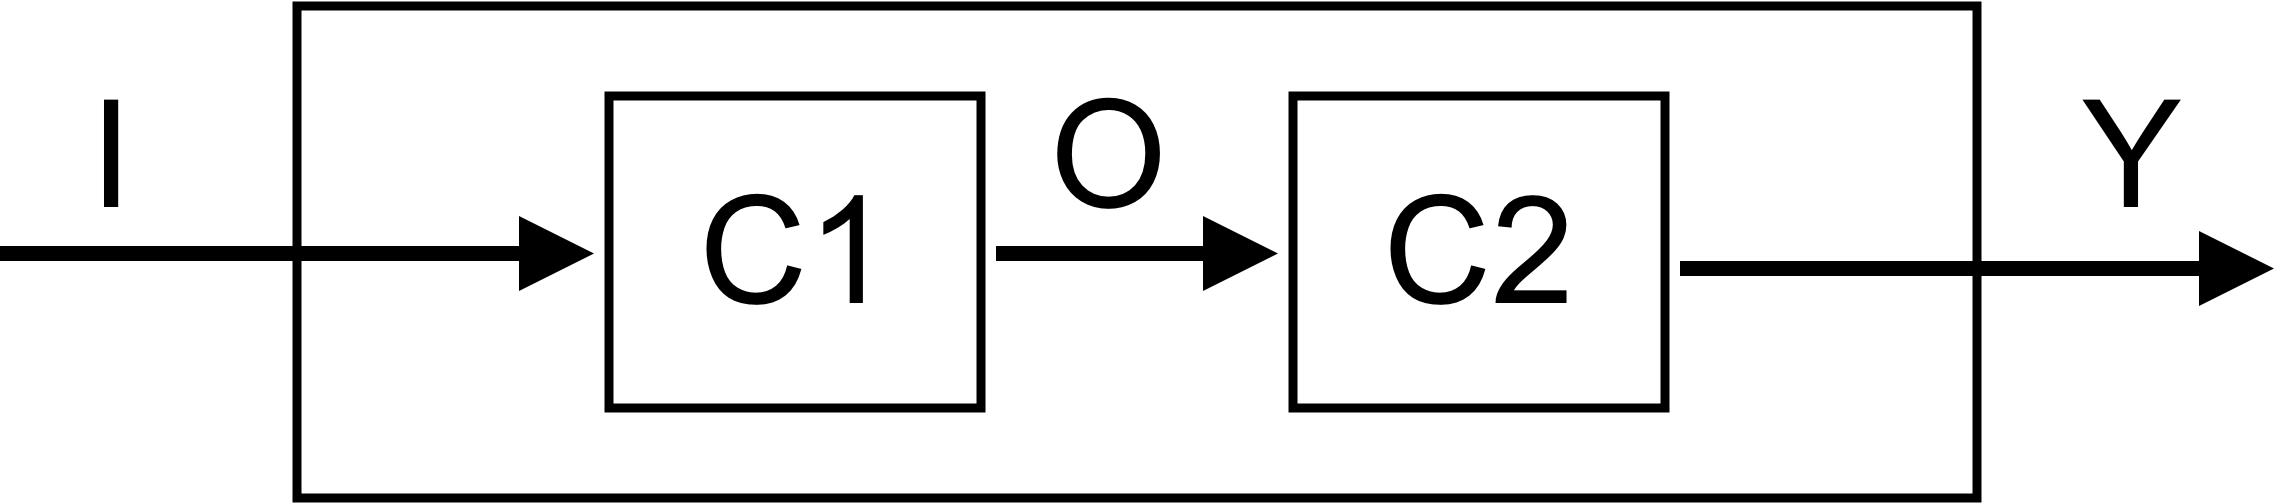
\includegraphics[width=0.4\textwidth]{figures/API-concat-operator.png}
	\end{center}
	\caption{Linear composition operator \code{concat}}
	\label{fig:concat-operator}
\end{figure}

It should be clear by now that given a value of type \code{I}, component \code{c1} should transform this into a value\footnote{Notice that the transformation in \code{c1} can also cause the output to return multiple values over time or no values at all.} of type \code{O}. This value is then used as the input of component \code{c2}, which in turn transforms it into a value of type \code{Y}. This value is then emitted as the output of the composed component. Besides these \code{OnNext} events, the \obs in either component can return an \code{OnError} or \code{OnCompleted} event. In this case the component not only has to propagate these events to the next component, but also needs to signal upstream that it is terminating. This means that the \subj which is inside the \comp can unsubscribe itself from every observer, and do this for all upstream components as well.

The behavior for regular \code{OnNext} events can be achieved by connecting the various streams in \Cref{fig:concat-operator} by subscribing them to each other. Notice that we have to connect the components in reversed order; that is, first subscribe the output of \code{c2} to the output of the composed component, then subscribe the output of \code{c1} to the input of \code{c2} and finally subscribe the input of the composed component to the input of \code{c1}. The reason for this is that either \code{c1} or \code{c2} might have elements that emit immediately when the stream is subscribed. Due to the nature of a \subj, these events would get lost if the \comp did not yet subscribe its output to something else.

The behavior of the terminal events can be achieved by using the functionality of Rx to compose subscriptions. In RxMobile every \obv is a \subs as well and likewise every \comp is an \obv, so we just need to \textit{add} the subscriptions to each other. To do so, we also require the subscription that represents the output of the \comp to be created. We get this by creating a new \obs and using the \obv in the lambda expression for this.

\begin{minipage}{\linewidth}
\begin{lstlisting}[style=ScalaStyle, caption={Linear composition operator \code{concat}}, label={lst:concat-operator}]
implicit class Operators[I, O](val src: Component[I, O]) {
  def concat[Y](other: Component[O, Y]): Component[I, Y] $=$ {
    val result $=$ Component[I, Y](input $\Rightarrow$ Observable.create(output $\Rightarrow$ {
      other.asObservable.subscribe(output)
      src.asObservable.subscribe(other)
      input.subscribe(src)

      output $+=$ other
      other $+=$ src
    }))
    src $+=$ result
    result
  }
}
\end{lstlisting}
\end{minipage}

\subsubsection{Abstracting over composition}
As we will use this feature of combining the \subs with the \comp to be created, we will already abstract over this and use this in upcoming operators as well.

\begin{minipage}{\linewidth}
\begin{lstlisting}[style=ScalaStyle, caption={\code{lift} operator}, label={lst:lift-operator}]
def lift[X, Y](f: (Observable[X], Observer[Y])$\Rightarrow$Unit): Component[X, Y] $=$ {
  val result $=$ Component[X, Y](input $\Rightarrow$ Observable.create(f(input, _)))
  src $+=$ result
  result
}
\end{lstlisting}
\end{minipage}

We can then use \code{lift} in \code{concat} as follows:

\begin{minipage}{\linewidth}
\begin{lstlisting}[style=ScalaStyle, caption={Revised implementation of the \code{concat} operator}, label={lst:concat-revised}]
implicit class Operators[I, O](val src: Component[I, O]) {
  def concat[Y](other: Component[O, Y]): Component[I, Y] $=$ {
    src.lift((input, output) $\Rightarrow$ {
      other.asObservable.subscribe(output)
      src.asObservable.subscribe(other)
      input.subscribe(src)

      output $+=$ other
      other $+=$ src
    })
  }
}
\end{lstlisting}
\end{minipage}

In general \code{lift} can be viewed as the creation of a new, encapsulating \comp, whose behavior is defined in the function \code{f}. The function arguments of types \obs and \obv represent the input and output of this new \comp respectively. This may seem counterintuitive at first, as a \comp has an input of type \obv and an output of type \obs. However, these types are what we see while looking at a \comp from the outside, whereas within the \code{lift} operator, we are looking at it from the inside. In that case the input has type \obs, since we want to receive new events and the output has type \obv, as we want to send new events.

\subsubsection{Formalizing the operators}
Before we continue developing new operators, we have to observe that both \code{concat} and \code{apply}/\code{create} satisfy the \textit{Arrow} type class that was described first in 2000 in a paper by John Hughes \cite{hughes2000-arrows}. The \textit{Arrow}  type class has similar operators to the \code{Monad} type class, but is defined more generally. Computations that are clearly not a monad can be composed over in the same way as computations that are a monad using this new type class. Just as a monadic type \code{M[A]} is representing a computation that delivers an \code{A}, so an arrow type \code{A[B, C]} is representing a computation with input \code{B} and output \code{C}. With that the dependence on the input of the computation is made explicit.

The \textit{Arrow} type class defines a couple of functions which are listed in \Cref{lst:arrow-typeclass} in Haskell. First of all, it defines \code{arr} to be a function that accepts a function from \code{b} to \code{c} as its input and the arrow from \code{b} to \code{c} as its output. This function is completely analogous to the \code{apply} method described earlier, where \code{b} and \code{c} are both of type \obs. Besides that, \textit{Arrow} defines the \code{(>>>)} operator, which composes two arrows together into one single arrow. Here the output of the first arrow is used as an input for the second arrow. This is of course analogue to the \code{concat} operator we just implemented. We define \code{(>>>)} as a second way of writing a linear composition.

\begin{minipage}{\linewidth}
\begin{lstlisting}[style=HaskellStyle, caption={\textit{Arrow} type class}, label={lst:arrow-typeclass}]
class Arrow a where
    arr :: (b $\rightarrow$ c) $\rightarrow$ a b c
    (>>>) :: a b c $\rightarrow$ a c d $\rightarrow$ a b d
\end{lstlisting}
\end{minipage}

\subsubsection{Parallel composition}
The careful reader may either have noticed that the definition of an arrow as provided in \Cref{lst:arrow-typeclass} is not complete or wonder how to implement an \code{add} function in arrow style. As Hughes shows, this is simple in a monadic context, but the current functions in the \textit{Arrow} type class do not satisfy the need.

\begin{lstlisting}[style=InlineHaskellStyle]
add :: Arrow a $\Rightarrow$ (a b Int) $\rightarrow$ (a b Int) $\rightarrow$ (a b Int)
add x y = $\ldots$
\end{lstlisting}

The input type \code{b} of the resulting arrow of this function needs to supply its value to both inputs of this functions arguments and combine its outputs. This is however not possible with the current \code{(>>>)} operator we have defined. Hence we require some new operators to be added to the \textit{Arrow} type class. Hughes defines these operators in terms of each other, leaving only one operator open that requires a custom implementation.

\begin{minipage}{\linewidth}
\begin{lstlisting}[style=HaskellStyle, caption={\textit{Arrow} type class}, label={lst:arrow-typeclass-full}]
class Arrow a where
    arr :: (b $\rightarrow$ c) $\rightarrow$ a b c
    (>>>) :: a b c $\rightarrow$ a c d $\rightarrow$ a b d
    first :: a b c $\rightarrow$ a (b,d) (c,d)
    
    second :: a b c $\rightarrow$ (d,b) (d,c)
    second f = arr swap >>> first f >>> swap
      where swap (x,y) = (y,x)
      
    (***) :: a b c $\rightarrow$ a d e $\rightarrow$ a (b,d) (c,e)
    f *** g = first f >>> second g
    
    (&&&) :: a b c $\rightarrow$ a b d $\rightarrow$ a b (c,d)
    f &&& g = arr ($\lambda$b $\rightarrow$ (b,b)) >>> (f *** g)
\end{lstlisting}
\end{minipage}

The operator \code{first} takes an arrow from \code{b} to \code{c} as its argument and just adds an extra input and output to the resulting arrow. \code{second} does the same, but effectively in reverse, by putting the extra input and output in the first slot. Note how it is possible to implement \code{second} in terms of \code{first} by doing extra swaps of the arguments.

\begin{figure}[H]
	\centering
	\begin{subfigure}[b]{0.35\linewidth}
		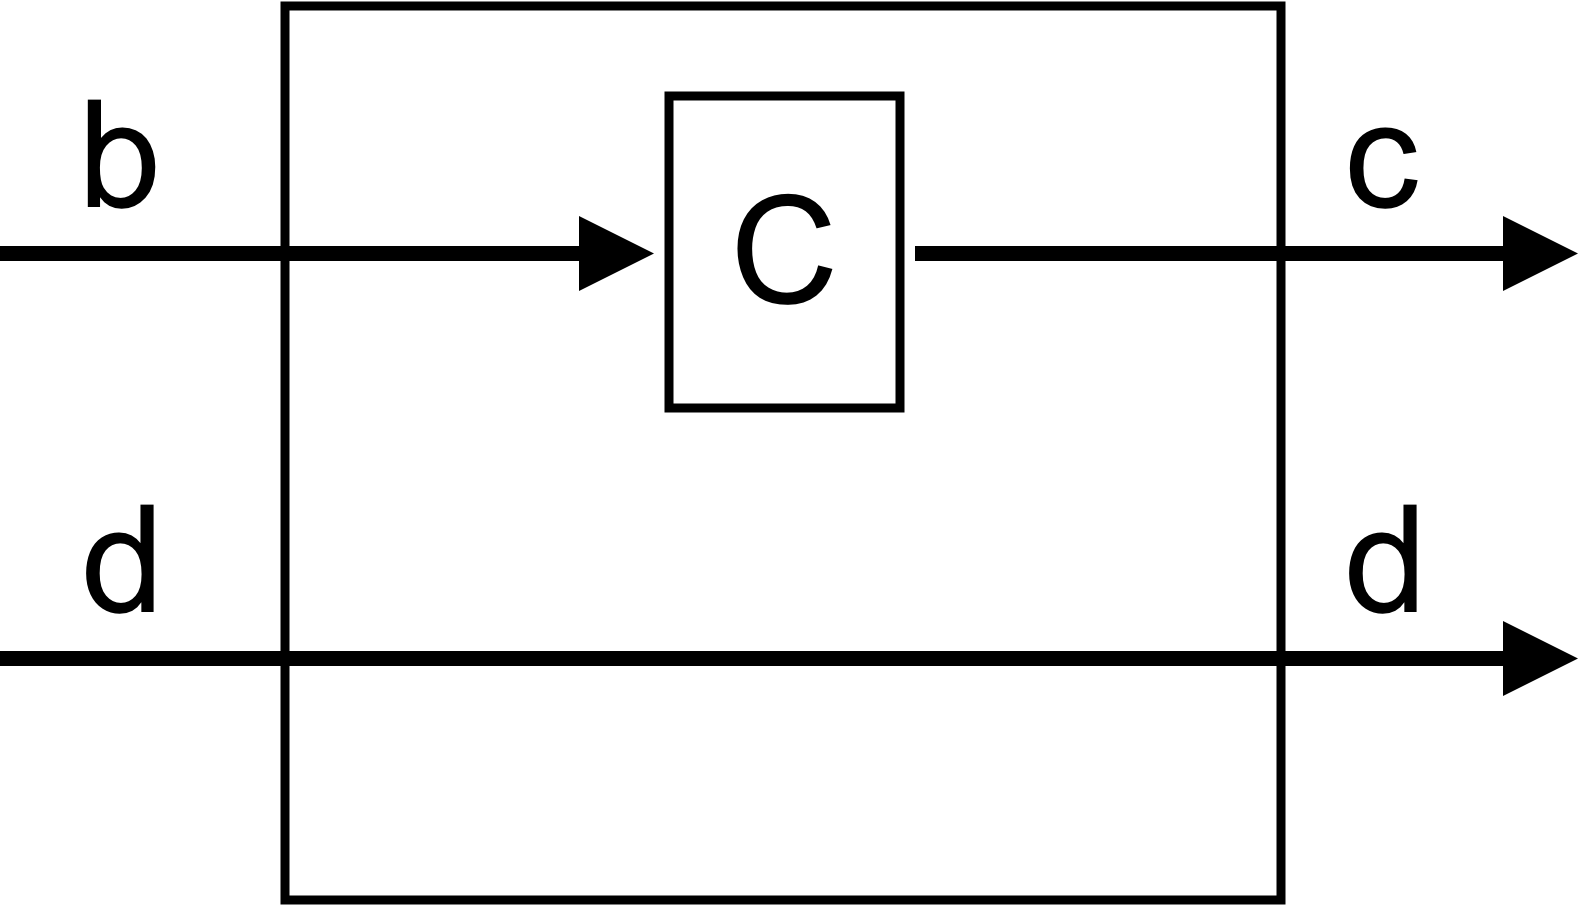
\includegraphics[width=\linewidth]{figures/API-first-operator.png}
		\caption{\code{first}}
		\label{fig:first-operator}
	\end{subfigure}
	\begin{subfigure}[b]{0.35\linewidth}
		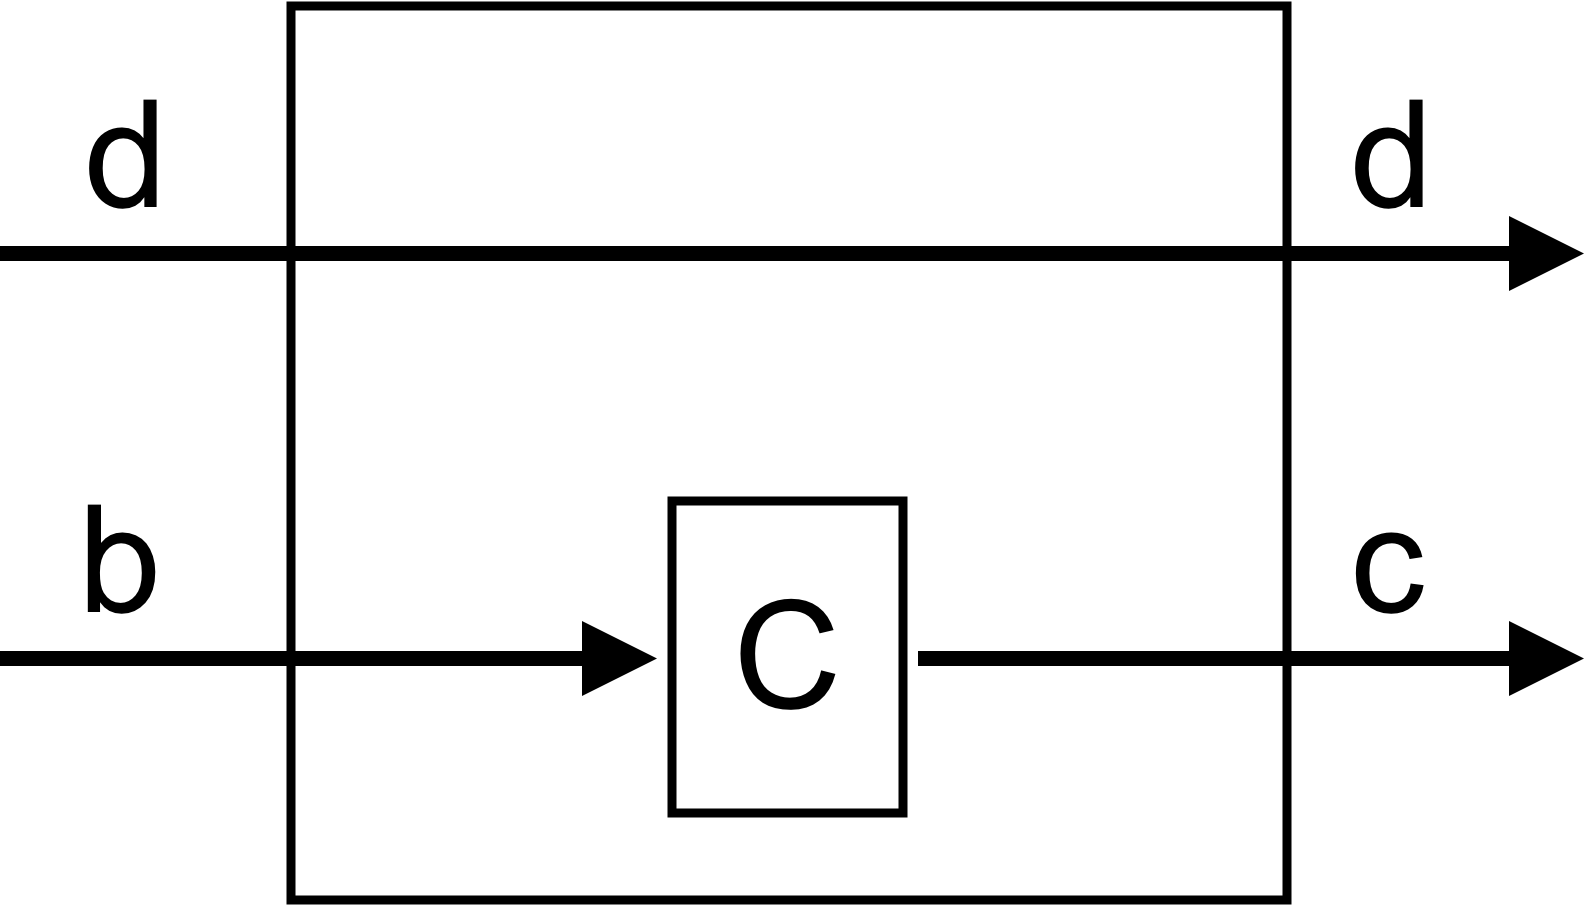
\includegraphics[width=\linewidth]{figures/API-second-operator.png}
		\caption{\code{second}}
		\label{fig:second-operator}
	\end{subfigure}
	
	\begin{subfigure}[b]{0.35\linewidth}
		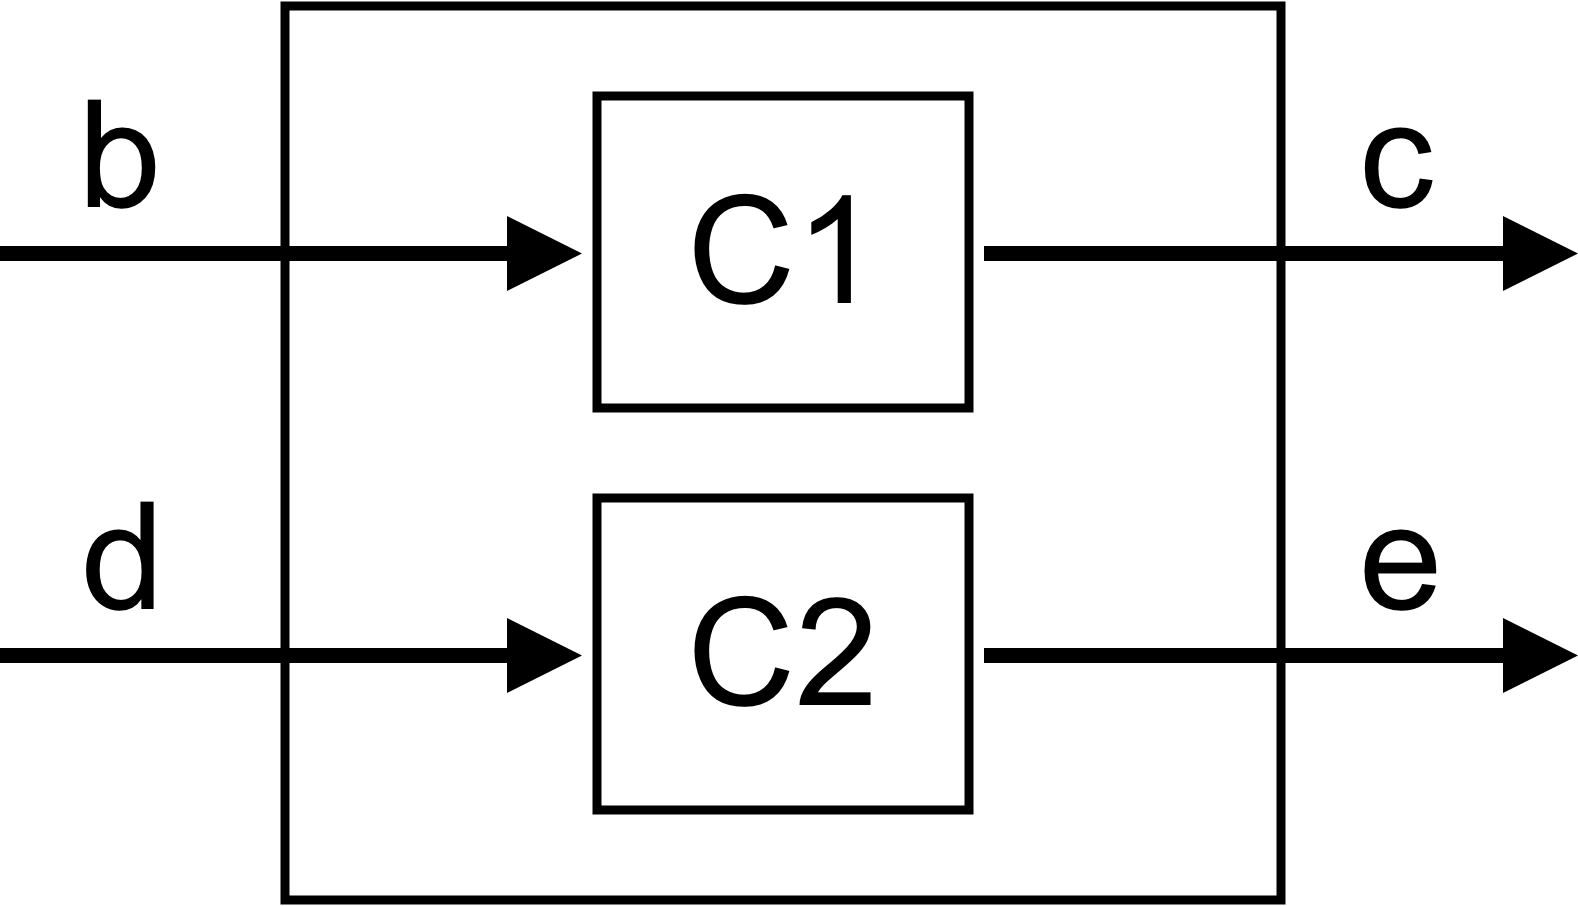
\includegraphics[width=\linewidth]{figures/API-split-operator.png}
		\caption{\code{(***)} or \code{split}}
		\label{fig:split-operator}
	\end{subfigure}
	\begin{subfigure}[b]{0.35\linewidth}
		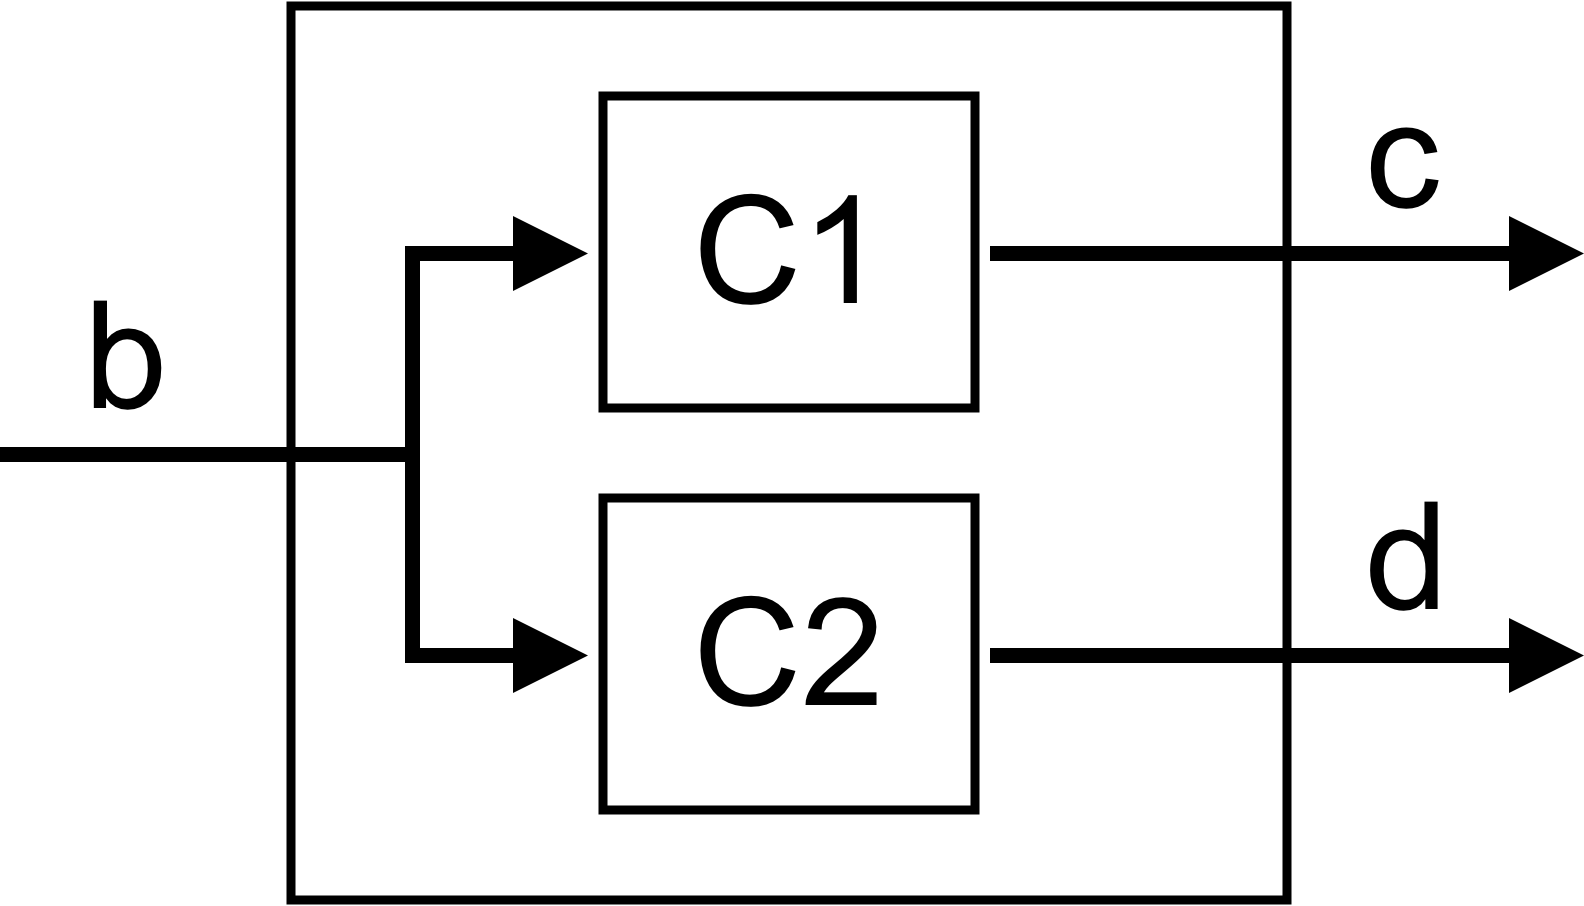
\includegraphics[width=\linewidth]{figures/API-fanout-operator.png}
		\caption{\code{(\&\&\&)} or \code{fanout}}
		\label{fig:fanout-operator}
	\end{subfigure}
	\caption{Parallel composition operators}
	\label{fig:parallel-composition}
\end{figure}

Implementing these two operators for \comp requires us to split the `\textit{input tuple stream}', apply the given \comp to the first part of this stream and merge it back with the second part of the stream. However, remember that for \obs there are a number of distinct operators for merging streams, each having their own behavior: \code{flatMap}, \code{combineLatest}, \code{withLatestFrom}, \code{zip}, \code{merge}, \code{concat}, etcetera. Since we want to merge the \comp's output stream and the second part of the input stream one-by-one, the \code{zip} operator is required here. The rest of the implementation details are just straightforward, using the earlier defined \code{lift} and taking care of the required subscriptions.

\begin{minipage}{\linewidth}
\begin{lstlisting}[style=ScalaStyle, caption={Implementations of the \textit{Arrow}'s \code{first} and \code{second} operators}, label={lst:first-and-second}]
implicit class Operators[I, O](val src: Component[I, O]) {
  $\ldots$

  def first[Y]: Component[(I, Y), (O, Y)] $=$ {
    src.lift((input, downstream) $\Rightarrow$ {
      val srcOut $=$ src.asObservable
      val inputOut $=$ input.map(_._2)

      input.map(_._1).subscribe(src)
      srcOut.zipWithBuffer(inputOut)((_, _)).subscribe(downstream)

      downstream $+=$ src
    })
  }

  def second[Y]: Component[(Y, I), (Y, O)] $=$ {
    Component.create[(Y, I), (I, Y)](_.swap) >>> src.first >>> Component.create(_.swap)
  }
}
\end{lstlisting}
\end{minipage}

The other two operators that Hughes defines for the \textit{Arrow} type class are \code{(***)} and \code{(\&\&\&)}. The former operator is used in ``\textit{parallel composition}'' of arrows, taking its input consisting of two arrows and merging them into one arrow of tuples. This is done by applying \code{first} to the first input argument and \code{second} to the second. The latter operator, takes this behavior one step further by specifying that the input type of both input arrows must be the same. With this we can construct a resulting arrow that has an input type \code{b}, whose values are supplied to both arrows, and an output type which is the tuple (or product) of both arrow's results. This type of composition is sometimes referred to as ``\textit{fanout composition}''. Implementations of these operators in the context of \comp are equivalent to the ones in \Cref{lst:arrow-typeclass-full}:

\begin{minipage}{\linewidth}
\begin{lstlisting}[style=ScalaStyle, caption={Implementations of the \textit{Arrow}'s \code{(***)} and \code{(\&\&\&)} operators}, label={lst:parallel-and-fanout}]
implicit class Operators[I, O](val src: Component[I, O]) {
  $\ldots$

  def ***[X, Y](other: Component[X, Y]): Component[(I, X), (O, Y)] $=$ {
    src.first[X] >>> other.second[O]
  }

  def &&&[Y](other: Component[I, Y]): Component[I, (O, Y)] $=$ {
    Component.create[I, (I, I)](b $\Rightarrow$ (b, b)) >>> (src *** other)
  }
}
\end{lstlisting}
\end{minipage}

Using these new operators, we are now able to define the \code{add} function in arrow style as described above. We compose the two arrows using a fanout and bring the two results together by using another component that adds the two values together. Notice that this function would be particularly interesting when implementing a PID controller or any other parallel composed set of components.

\begin{lstlisting}[style=InlineHaskellStyle]
add :: Arrow a $\Rightarrow$ (a b Int) $\rightarrow$ (a b Int) $\rightarrow$ (a b Int)
add x y = (x &&& y) >>> arr ($\lambda$(b,c) $\rightarrow$ b + c)
\end{lstlisting}

Hughes finishes this trail by generalizing the \code{add} to a \code{liftA2}, which is equivalent in functionality to Haskell's \code{liftM2} which combines the results of two monadic computations. Besides two input arrows, \code{liftA2} accepts a combinator function that is applied after the fanout composition of the two arrows. We define a similar operator called \code{combine} in our API for the purpose of parallel composition:

\begin{minipage}{\linewidth}
\begin{lstlisting}[style=ScalaStyle, caption={Implementation of the \code{Arrow}'s \code{liftA2} or \code{combine} operator}, label={lst:combine-operator}]
implicit class Operators[I, O](val src: Component[I, O]) {
  $\ldots$

  def combine[X, Y](other: Component[I, X])(combiner: (O, X) $\Rightarrow$ Y): Component[I, Y] $=$ {
    (src &&& other) >>> Component.create(combiner.tupled)
  }
}
\end{lstlisting}
\end{minipage}

\subsubsection{Problems with parallel composition on \comp}
Although our implementation of these parallel composition operators in the context of \comp might seem fine at first glance, the observant reader might have spotted some flaws in it. The main concern here is the choice of using \code{zip} in the \code{first} operator. As discussed in section \Cref{sec:fastproc-slowcons}, \code{zip} is particularly risky to use given the unpredictable nature of its source streams. This same danger comes up in our implementation of \code{first}, as the inner component might produce more than one element for every received element or as it might start with a certain number of elements before producing elements based on what it receives\footnote{This can be achieved using \code{startWith}, which is a well-known operator for \obs and which we will introduce later in the context of \comp.}.

Besides that, given that \code{zip} is used in the \code{first} operator, it follows that it is also used in \code{second} and that it is technically used twice in \code{(***)}, \code{(\&\&\&)} and \code{combine}. This is not only twice as risky, but is also fairly inefficient as the underlying Rx code needs to maintain two queues now. We will show that this can be done more efficiently by reducing the uses of \code{zip} to only once per \code{combine} operation.

For this we have to observe that we can not only implement \code{(***)} in terms of \code{first} and \code{second} but that it is also possible to implement both \code{first} and \code{second} in terms of \code{(***)}! After all, \code{first} is completely equal to \code{(***)} with the second input arrow being the identity. We can easily see this by comparing \Cref{fig:first-operator} to \Cref{fig:split-operator} where \code{c2} is equal to \code{Component.identity}. The same is true for \code{second} by making \code{c1} in \Cref{fig:split-operator} the identity \comp.

The \code{(***)} operator can then be implemented in terms of \code{lift} by splitting the input stream and subscribing both parts to the first and second component respectively. Then the outputs of these components are zipped together into a tuple and subscribed to the output of the resulting \comp. After that we are only left with some administrative work in terms of the subscriptions.

The other operators, \code{(\&\&\&)} and \code{combine} do not require any modifications as they were already implemented in terms of \code{(***)}. The full implementation of the parallel composition operators in our API now looks as follows:

\begin{minipage}{\linewidth}
\begin{lstlisting}[style=ScalaStyle, caption={New implementation of the \textit{Arrow}'s operators}, label={lst:new-arrow-implementation}]
implicit class Operators[I, O](val src: Component[I, O]) {
  $\ldots$

  def first[Y]: Component[(I, Y), (O, Y)] $=$ {
    src *** Component.identity[Y]
  }

  def second[Y]: Component[(Y, I), (Y, O)] $=$ {
    Component.identity[Y] *** src
  }

  def ***[X, Y](other: Component[X, Y]): Component[(I, X), (O, Y)] $=$ {
    src.lift((input, downstream) $\Rightarrow$ {
      input.map(_._1).subscribe(src)
      input.map(_._2).subscribe(other)

      src.asObservable.zipWithBuffer(other.asObservable)((_, _)).subscribe(downstream)

      downstream $+=$ src
      downstream $+=$ other
    })
  }

  def &&&[Y](other: Component[I, Y]): Component[I, (O, Y)] $=$ {
    Component.create[I, (I, I)](b $\Rightarrow$ (b, b)) >>> (src *** other)
  }

  def combine[X, Y](other: Component[I, X])(combiner: (O, X) $\Rightarrow$ Y): Component[I, Y] $=$ {
    (src &&& other) >>> Component.create(combiner.tupled)
  }
}
\end{lstlisting}
\end{minipage}

\subsubsection{Functor, Applicative, Monad}
One of the reasons that Hughes introduced the \textit{Arrow} \cite{hughes2000-arrows} is that he saw that not all kinds of computations can be described in terms of monads. He uses the parser library by Swierstra and Duponcheel \cite{swierstra1996-parsers} as an example of a structure that can implement the choice combinator from the \textit{MonadPlus} type class but turns out to have no possible implementation for the \textit{Monad}'s \code{(>>=)} operator. Their solution to this problem is to discard the use of a \textit{Monad} and instead use a different operator \code{(<*>)} that later became known as part of the \textit{Applicative} type class. Nowadays \textit{Applicative} sits right in the middle between \textit{Functor} and \textit{Monad} and \textit{MonadPlus} not only `inherits' from \textit{Monad} but also from \textit{Alternative}, which already has the choice combinator (see \Cref{lst:type-classes-for-monads}).

As an alternative to introducing the \code{(<*>)} operator as Swierstra and Duponcheel did, Hughes introduces the \textit{Arrow} as the answer to combining non-monadic computations. With this he shows that every \textit{Monad} is in fact an \textit{Arrow}, but that not every \textit{Arrow} is a \textit{Monad}. For this he introduces another type class \textit{ArrowApply} (\Cref{lst:arrow-apply}), which he shows to be equivalent to the \textit{Monad} type class. From this it follows that for an \textit{Arrow} to be also a \textit{Monad} it must be able to implement the \textit{ArrowApply} type class.

\begin{lstlisting}[style=HaskellStyle, caption={\textit{ArrowApply} type class}, label={lst:arrow-apply}, captionpos=b, numbers=none]
class Arrow a $\Rightarrow$ ArrowApply a where
  app :: a (a b c, b) c
\end{lstlisting}

\begin{minipage}{0.6\linewidth}
\begin{lstlisting}[style=HaskellStyle, caption={Monadic type classes}, label={lst:type-classes-for-monads}, captionpos=b, numbers=none]
class Functor f where
  fmap :: (a $\rightarrow$ b) $\rightarrow$ f a $\rightarrow$ f b

class Functor f $\Rightarrow$ Applicative f where
  pure :: a $\rightarrow$ f a
  (<*>) :: f (a $\rightarrow$ b) $\rightarrow$ f a $\rightarrow$ f b

class Applicative m $\Rightarrow$ Monad m where
  return :: a $\rightarrow$ m a
  (>>=) :: m a $\rightarrow$ (a $\rightarrow$ m b) $\rightarrow$ m b

class Applicative f $\Rightarrow$ Alternative f where
  empty :: f a
  (<$|$>) :: f a $\rightarrow$ f a $\rightarrow$ f a

class (Alternative m, Monad m) $\Rightarrow$ MonadPlus m where
  mzero :: m a
  mzero = empty
  
  mplus :: m a $\rightarrow$ m a $\rightarrow$ m a
  mplus = (<$|$>)
\end{lstlisting}
\end{minipage}
\begin{minipage}{0.4\linewidth}
	\begin{figure}[H]
		\begin{center}
			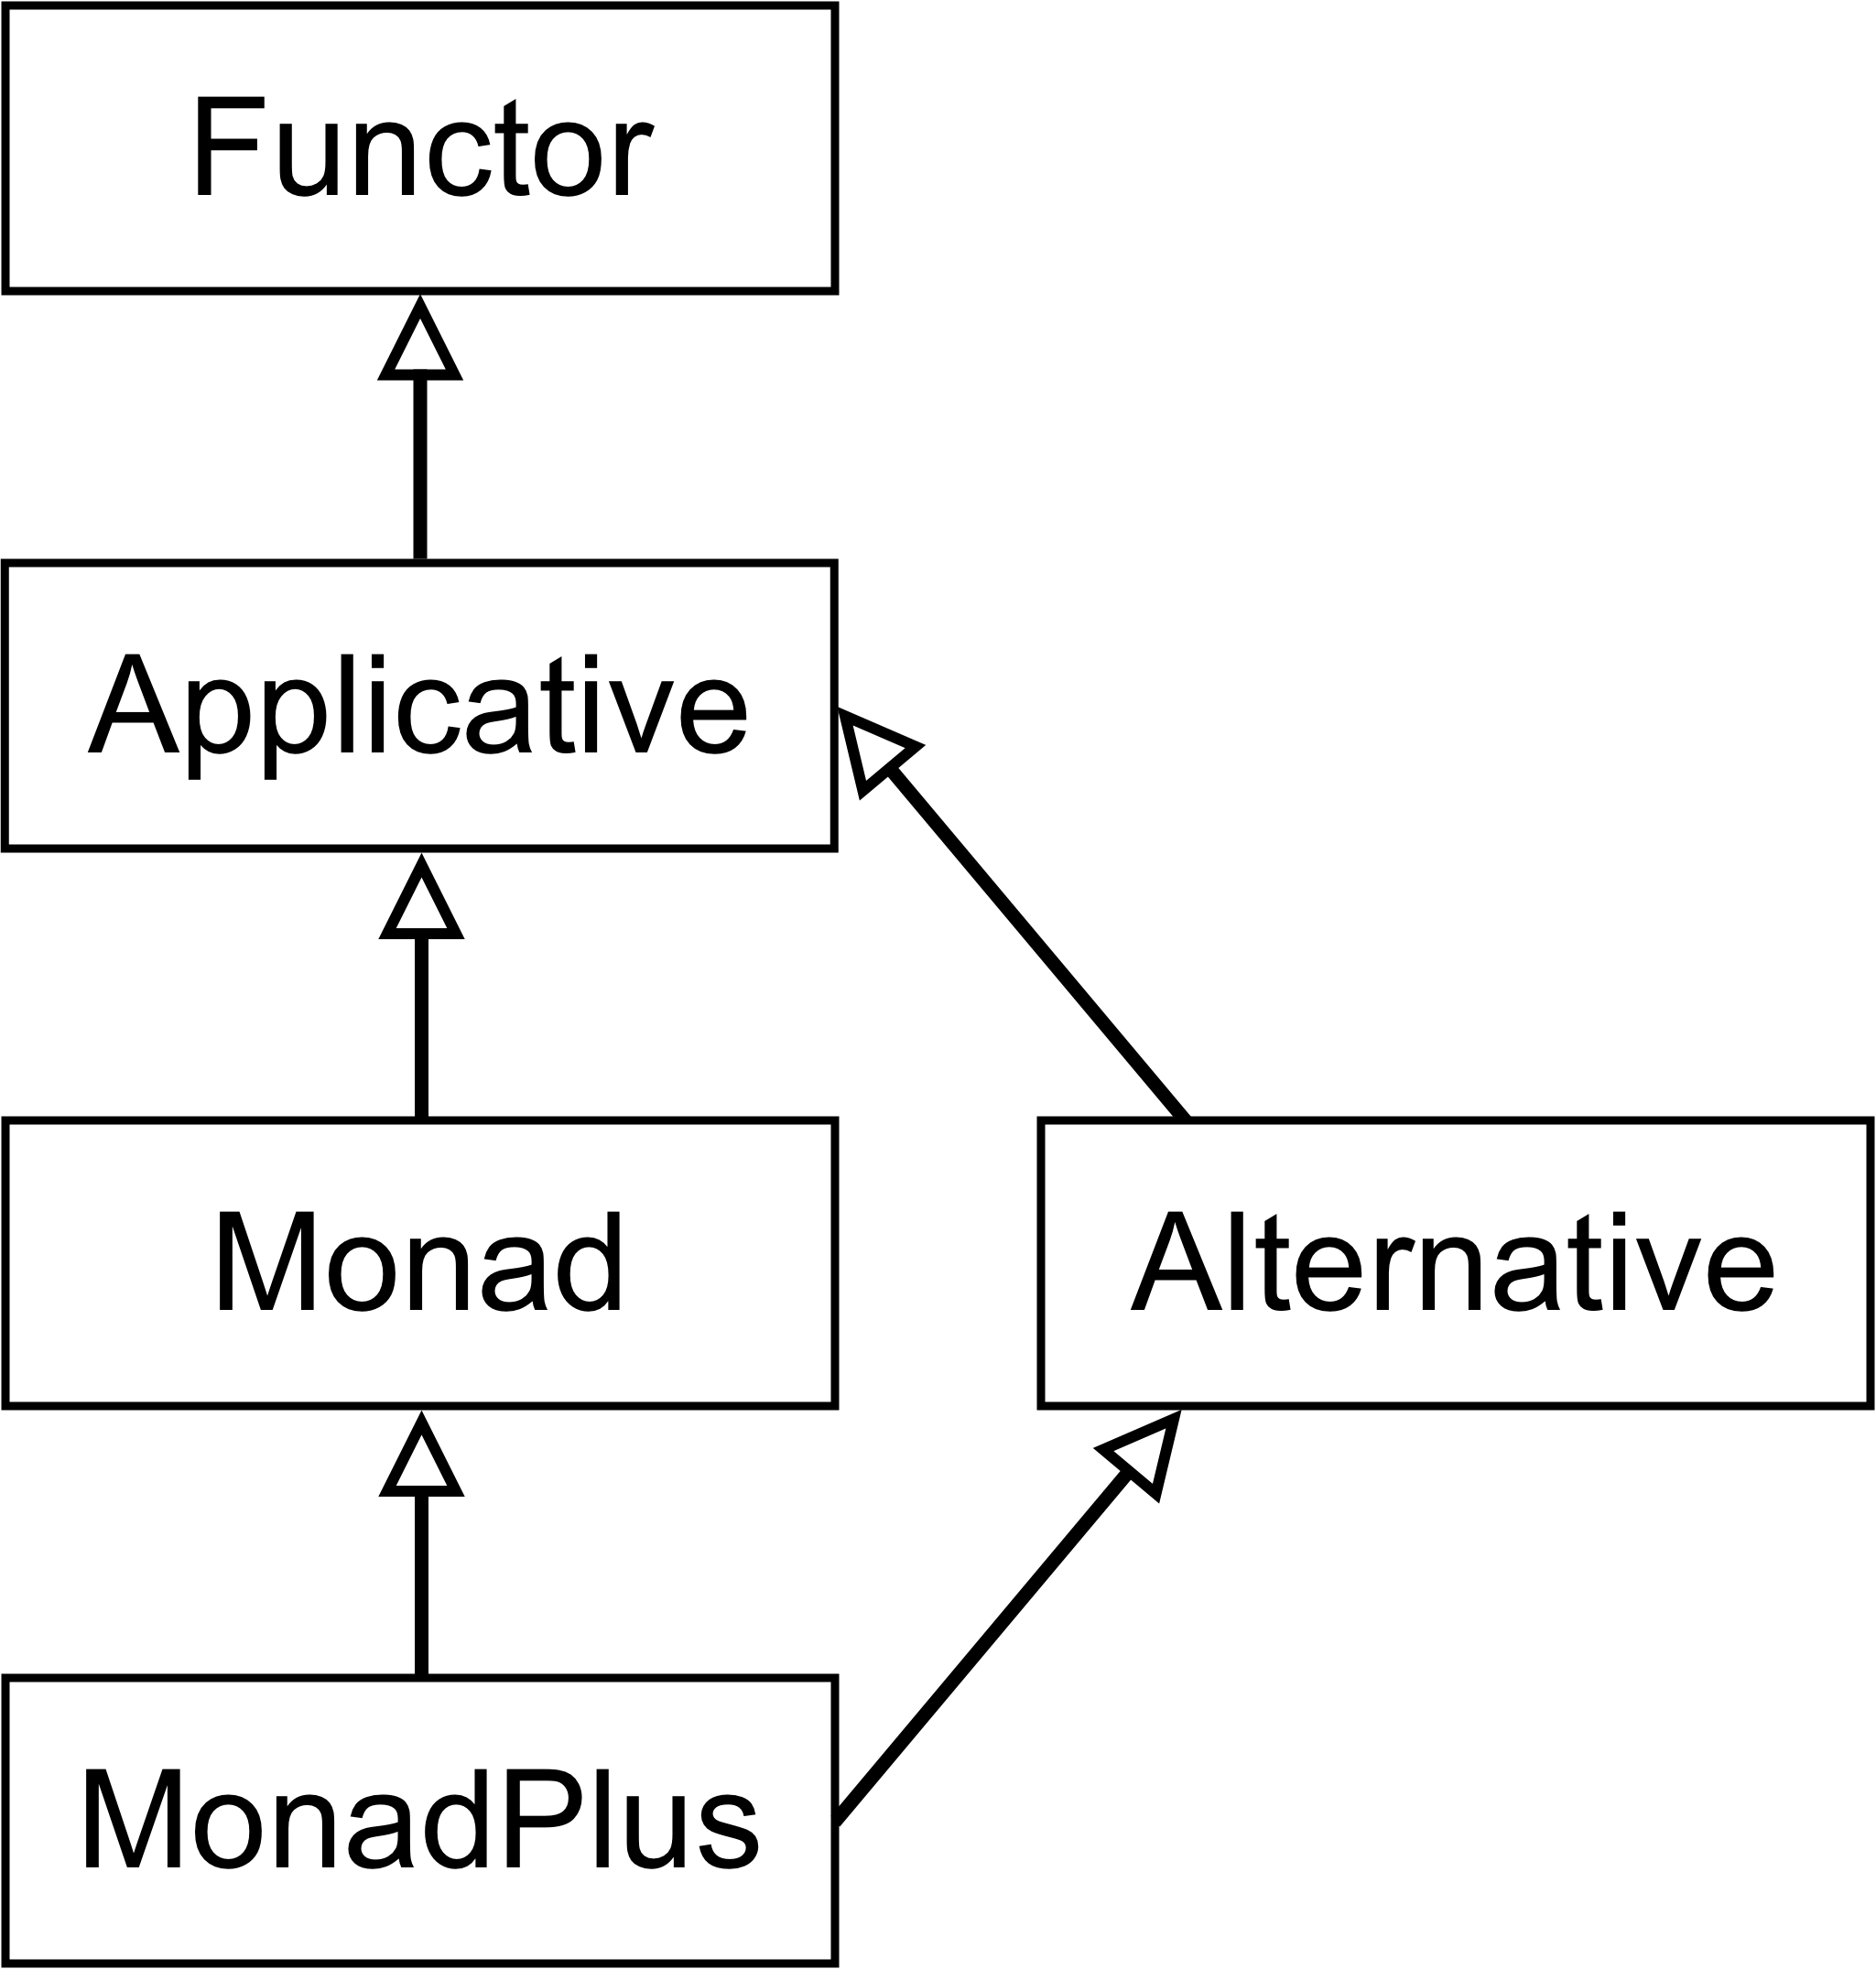
\includegraphics[width=\textwidth]{figures/Monadic-type-classes.png}
		\end{center}
		\caption{Monadic type classes}
		\label{fig:type-classes-for-monads}
	\end{figure}
\end{minipage}

In the previous sections we have demonstrated the \comp interface to be an \textit{Arrow}, which, given the discussion above, brings us to the question whether \comp is also a \textit{Functor}, \textit{Applicative} and \textit{Monad} and hence whether we are allowed to add the associated operators to our API.

The \textit{Functor} type class (\Cref{lst:type-classes-for-monads}) contains a single function \code{fmap} which accepts a \textit{Functor} and a function as its input and returns a new \textit{Functor} on which the function is applied. Translated to the \comp interface, \code{map}\footnote{\code{fmap} in Haskell is usually referred to in Scala as \code{map}} applies a transformation function to the output of the given \comp. This is simple, as we can already wrap a function in a \comp using the \code{create} operator and we can concatenate two components using \code{concat} or \code{(>>>)}.

The \textit{Applicative} type class (\Cref{lst:type-classes-for-monads}) contains two functions, \code{pure} and \code{(<*>)}. We already have the former function in our API, namely \code{from} (\Cref{lst:creating-component}). The latter function is almost the same as \code{fmap}, only with the difference that the function is wrapped inside an \textit{Applicative}. The two input parameters of \code{(<*>)} need to be merged into a single \textit{Applicative} where the function from the first parameter is applied to the value from the second parameter. We also already have this functionality in the form of the \code{combine} operator, which combines two instances of \comp using a given function.

\begin{minipage}{\linewidth}
\begin{lstlisting}[style=ScalaStyle, caption={\textit{Functor} and \textit{Applicative} operators}, label={lst:functor-and-applicative}]
implicit class Operators[I, O](val src: Component[I, O]) {
  $\ldots$

  def map[X](f: O $\Rightarrow$ X): Component[I, X] $=$ src >>> Component.create(f)
  
  def <*>[X, Y](other: Component[I, X])(implicit ev: O $<:<$ (X $\Rightarrow$ Y)): Component[I, Y] $=$ {
    src.combine(other)(ev(_)(_))
  }
}
\end{lstlisting}
\end{minipage}

Contrary to the previous type classes, it turns out that we are not able to implement the \textit{Monad}'s \code{(>>=)} (or \code{flatMap}) operator. Note that this is equivalent to saying that we are unable to implement the \textit{ArrowApply}'s \code{app} operator. Writing down these definitions shows how non-sensible both these definitions are:

\begin{lstlisting}[style=InlineScalaStyle]
implicit class MonadOperators[I, O](val src: Component[I, O]) {
  def flatMap[X](f: O $\Rightarrow$ Component[I, X]): Component[I, X]
  def app(implicit ev: I $<:<$ (Component[I, O], I)): Component[I, O]
}
\end{lstlisting}

From the perspective of \code{flatMap} it would mean that every time \code{src} produces an output, it is fed to the function \code{f}, which would produce a completely new \comp to be subscribed to the result of \code{flatMap}. This would mean that after $n$ outputs, there are $n$ \comp which are `dynamically' created and that the resulting component will emit $n$ values. The same holds for \code{app}, which would receive a new \comp to invoke with every input it receives.

The fact that \comp is not a monad may seem surprising at first, but is actually supported by Hughes, who gives an example of stream processing (which is similar in behavior to our API, but very different in its implementation) and also concludes that stream processing cannot be fitted into the monadic framework \cite{hughes2000-arrows}. He concludes that this is again an example of why not every instance of an \textit{Arrow} type class is automatically a \textit{Monad} as well.

\subsubsection{Reactive operators}
Since the \comp interface is written in terms of Rx, we may also want to use some of the operators that are defined on \obs. For example, a components may be a filter or just the functionality that it will skip the first $n$ elements it receives or start by emitting a certain value before responding to the \comp's actual input.

One way of doing this would be to create new components for each of these operations as they are needed while writing the feedback system and performing linear composition on these components. However, this would reduce the expressiveness and readability of the program that is written and would mean a lot of repeats of the same code: \code{x >>> Component(\char`_.$operator1$) >>> Component(\char`_.$operator2$)}.

A better way of doing this would be to add the most commonly used operators to the \comp API. By doing so, we can eliminate writing a lot of the same code, make the API more pleasant to use and improve the readability of the code. In fact, we have already introduced one operator that is also an operator in the Rx libraries and follows the implementation pattern as shown above: \code{map} (\Cref{lst:functor-and-applicative}).

Because the implementations of these operators will be almost identical in every case, we first introduce an operator \code{liftRx} (\Cref{lst:rx-style-operators}), which lifts an Rx operator into the \comp API such that it can be used in the API as a proper operator. This not only serves the purpose of eliminating duplicate code in the API but can also be used to have a way of lifting an Rx operator that is not present in our API.

Some of the operators present in the API are listed in \Cref{lst:rx-style-operators}, though many more can be thought of to be added.

\begin{minipage}{\linewidth}
\begin{lstlisting}[style=ScalaStyle, caption={Rx style operators}, label={lst:rx-style-operators}]
implicit class Operators[I, O](val src: Component[I, O]) {
  $\ldots$

  def liftRx[Y](f: Observable[O] $\Rightarrow$ Observable[Y]) $=$ src >>> Component(f)
  
  def drop(n: Int): Component[I, O] $=$ liftRx(_.drop(n))
  def filter(predicate: O $\Rightarrow$ Boolean): Component[I, O] $=$ liftRx(_.filter(predicate))
  def map[X](f: O $\Rightarrow$ X): Component[I, X] $=$ liftRx(_.map(f))
  def sample(interval: Duration, scheduler: Scheduler $=$ NewThreadScheduler()) $=$ liftRx(_.sample(interval, scheduler))
  def startWith(o: O): Component[I, O] $=$ liftRx(_.startWith(o))
  def scan[Y](seed: Y)(combiner: (Y, O) $\Rightarrow$ Y): Component[I, Y] $=$ liftRx(_.scanLeft(seed)(combiner))
  def take(n: Int): Component[I, O] $=$ liftRx(_.take(n))
  def throttle(duration: Duration, scheduler: Scheduler $=$ NewThreadScheduler()) $=$ liftRx(_.throttle(duration, scheduler))
}
\end{lstlisting}
\end{minipage}

Given these new operators, we can reimplement the \code{RunningAverage} example from \Cref{lst:running-average-final}. As all will agree, this looks much better and makes the code more readable and usable!

\begin{minipage}{\linewidth}
\begin{lstlisting}[style=ScalaStyle, caption={Implementation of \code{RunningAverage} using the new Rx style operators}, label={lst:running-average-with-operators}]
implicit class RunningAverageOperator(val src: Component[Double, Double]) {
  def runningAverage: Component[Double, Double] $=$ {
    src.scan(new Queue[Double]) { case (queue, value) $\Rightarrow$
        if (queue.length $==$ n)
          queue.dequeue()
        queue $+=$ value
      }
      .drop(1)
      .map(queue $\Rightarrow$ queue.sum / queue.size)
  }
}
\end{lstlisting}
\end{minipage}

\subsubsection{Feedback operator}
One of the most needed operations in building feedback systems is \textit{feedback}; the notion of feeding back a \comp's output to its input after merging it with the latest element of another stream, while also emitting the same output to the surrounding \comp (see \Cref{fig:feedback-operator}).

Though this may seem easy given the infrastructure that we have already build around our API, using \code{lift} and subscriptions, there are some technicalities that need to be taken into account in this implementation. First of all, in this situation there is a kind of recursion involved on the stream level. This needs some work as the recursed values' emissions need to be postponed to the appropriate moment rather than being emitted directly. Besides that, although the expected behavior of merging a \comp with \code{setpoint} can be naively implemented using a \code{withLatestFrom}, it turns out that this does not work in the case where \code{setpoint} emits its \emph{only} element before the \comp emits anything. This has to do with the behavior of \code{withLatestFrom} which discards everything that is emitted on the second \obs as long as the first \obs has not yet emitted any values.

The first concern, regarding the recursion, is solvable with the dedicated \code{TrampolineScheduler} which is available in both RxJava and RxMobile. This scheduler is specially created for recursive streams like this one and ``\textit{queues work on the current thread to be executed after the current work completes}'' \cite{RxJava-Trampoline-Scheduler}. As long as the stream that runs back into the input of the \comp is observed on this \sch (\Cref{lst:feedback-operator} \cref{line:observe-on-trampoline}), the recursion should work out fine.

The concern about an early emitting \code{setpoint} is somewhat harder to fix. To solve this, we have to do a \code{combineLatest} on these streams in order to not discriminate against which stream emits first. However, as soon as both streams have emitted their first value, we have to switch to the original \code{withLatestFrom} behavior. This is done in the function \code{loop} in \Cref{lst:feedback-operator} \cref{line:feedback-loop}. Here the first values of each of the two streams are merged into a tuple using the \code{combineLatest} and \code{take(1)}. Notice that the latter causes the stream to complete immediately after the first tuple is emitted. This \code{OnCompleted} is however postponed by \code{flatMap} until the inner-stream is completed. Inside the \code{flatMap} we unpack the tuple again and feed the values as the first new input of the \code{src} component. Here also the merging behavior is `replaced' by \code{withLatestFrom}. Due to our earlier concern with recursion, we have to use the extra \code{Observable.create} here and feed the first tuple to the \code{observer} by hand.

\begin{figure}[H]
	\begin{center}
		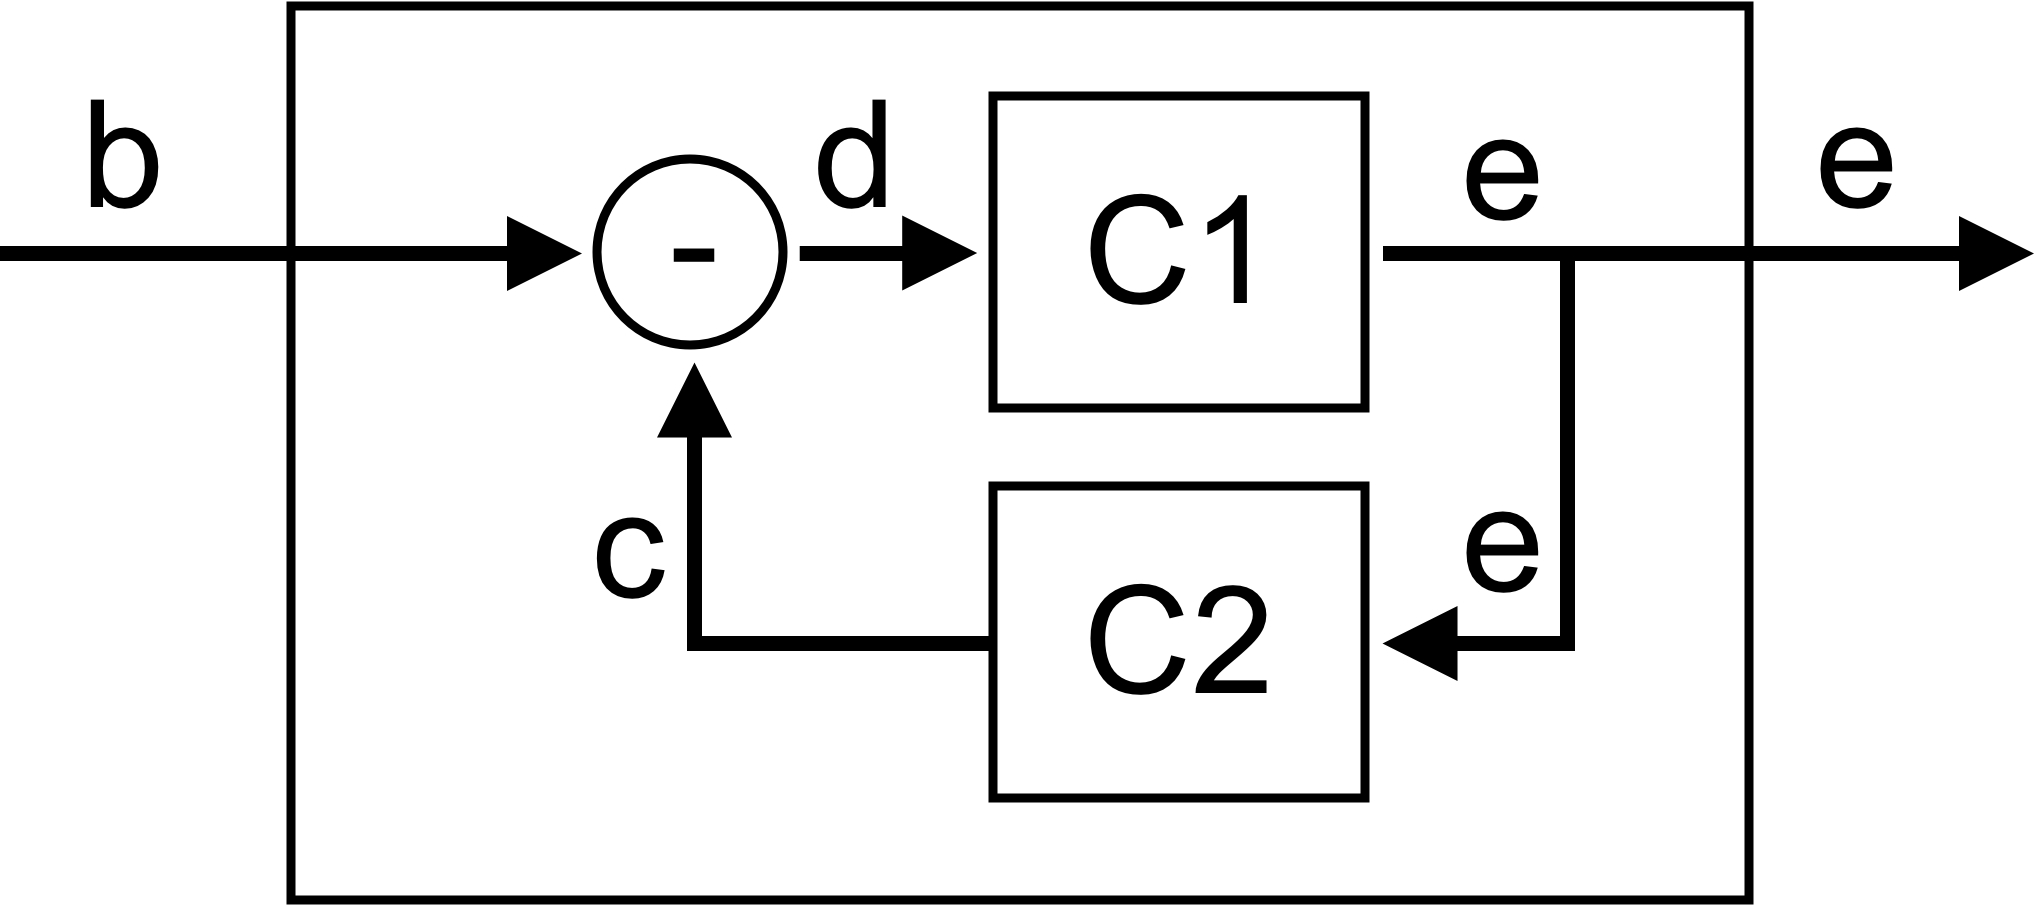
\includegraphics[width=0.4\textwidth]{figures/API-feedback-operator.png}
	\end{center}
	\caption{Feedback operator}
	\label{fig:feedback-operator}
\end{figure}

With the \code{loop} function in place, we can implement the \code{feedback} operator as shown in \Cref{lst:feedback-operator} \cref{line:feedback-operator}. As usual we use the \code{lift} operator as the basis of the implementation. Notice how we have to subscribe the output of \code{src} twice, once to the output of the encapsulating component (\code{downstream}) and once to the input of the transducer \code{trd}. Also notice that the order of subscriptions is important here: we first have to subscribe the output of the transducer to \code{src} (after applying the \code{loop} function and observing on the \code{TrampolineScheduler}) and only then subscribe the \code{src}'s output to both \code{downstream} and the transducer. Just as with \code{concat} this order of subscriptions prevents us from losing initial elements.

\begin{minipage}{\linewidth}
\begin{lstlisting}[style=ScalaStyle, caption={Feedback operator}, label={lst:feedback-operator}]
implicit class Operators[I, O](val src: Component[I, O]) {
  $\ldots$

  def feedback(f: O $\Rightarrow$ I)(implicit n: Numeric[I]): Component[I, O] $=$ {
    feedback(Component.create(f))
  }

  def feedback(tr: Component[O, I])(implicit n: Numeric[I]): Component[I, O] $=$ { |\label{line:feedback-operator}|
    lift((setpoint, downstream) $\Rightarrow$ {
      loop(tr.asObservable, setpoint)((t, s) $\Rightarrow$ n.minus(s, t))
        .observeOn(new TrampolineScheduler) |\label{line:observe-on-trampoline}|
        .subscribe(src)

      src $+=$ src.asObservable
        .publish(source $\Rightarrow$ {
          source.subscribe(downstream)
          source.subscribe(tr)

          source
        }).subscribe()

      downstream $+=$ src
      downstream $+=$ tr
      tr $+=$ src
    })
  }
  
  private def loop[T, S](transOut: Observable[T], setpoint: Observable[S]) (combinator: (T, S) $\Rightarrow$ I): Observable[I] $=$ { |\label{line:feedback-loop}|
    transOut.publish(tos $\Rightarrow$ setpoint.publish(sps $\Rightarrow$
      tos.combineLatest(sps)((_, _))
        .take(1)
        .flatMap { case (t, s) $\Rightarrow$
          Observable.create[I](observer $\Rightarrow$ {
            tos.withLatestFrom(sps.startWith(s))(combinator).subscribe(observer)
            observer.onNext(combinator(t, s))
          })
        }))
  }
}
\end{lstlisting}
\end{minipage}

With this last operator added to the API, we think we have a solid framework for creating and executing feedback systems that can be placed in production worthy systems. The interface as well as the set of operators have their foundations in theoretical concepts such as category theory and functional programming and are built on top of the very successful concept of reactive programming. It is our believe that this API can replace any imperatively created feedback system. We will use our API in \Cref{sec:reactive-balltracker} by revisiting the small \textit{ball movement control system} example from \Cref{sec:imperative-balltracker}.

\section{Improvements on the API}
The reader that is experienced with the concepts of Rx may have spotted an interesting point in the implementations of the operators in the previous section. This already becomes apparent from the implementation of \code{concat} in \Cref{lst:concat-operator,lst:concat-revised}. Although the purpose of this operator is to connect two instances of \comp in a linear composition, most of the work is spend on administrative work to subscribe streams to each other and add unsubscribe handlers. Also note again that the order in which these subscribe calls are executed is actually important!

One might argue that this is just how this operator is supposed to be set up for it to work correctly. The experienced Rx user will however respond to this by observing that all we are doing is connecting various instances of \subj in a somewhat complex manner. This is true, given the implementation of the \comp interface in \Cref{lst:component-v1}. As derived in \Cref{subsec:api-derivation}, a \comp must be an object that received elements of one type and internally transform these into another type and push out these new elements to those who are subscribed to it. Also we determined in \Cref{lst:component-v1} that the essence of \comp is the \code{transform} function which transforms a stream of elements of one type into a stream of elements of another type. This also becomes apparent in the \code{apply} function in \Cref{lst:creating-component}, which precisely has this transformation as its argument. The ceremony that is required to make this work in \Cref{lst:component-v1} involves the \subj, \obv and the associated subscription management that becomes visible in \Cref{lst:concat-operator,lst:concat-revised}.

The refactoring we propose in this section is to remove these ceremonial elements from the \comp interface and to really make the \code{transform} function the essence of the interface. For this we remove the \subj, the associated \code{\char`_subscription} value as well as the inheritance from \code{Observer[I]}. What we end up with is a simple class \comp with a \code{transform} function of type \code{Observable[I] $\Rightarrow$ Observable[O]} as its argument and in single method called \code{run} that transforms an input stream into an output stream (\Cref{lst:component-v2}). The associated \code{apply} function is changed accordingly.

\begin{minipage}{\linewidth}
\begin{lstlisting}[style=ScalaStyle, caption={Revised version of the \comp interface}, label={lst:component-v2}]
class Component[I, O](transform: Observable[I] $\Rightarrow$ Observable[O]) {

  def run(is: Observable[I]): Observable[O] $=$ transform(is)
}
object Component {
  def apply[I, O](transform: Observable[I] $\Rightarrow$ Observable[O]): Component[I, O] $=$
    new Component(transform)

  $\ldots$
}
\end{lstlisting}
\end{minipage}

Due to the way the operators are implemented we are forced to change only three of them, which we will refer to as the primative operators. These are \code{concat}, \code{(***)} and \code{feedback}. All the other operators are composed from these three operators and the \code{apply} function. The primative operators can be recognized in the previous section as those operators that were implemented in terms of \code{lift}. With the introduction of this revised version of \comp we will no longer have a need for \code{lift} and we can therefore discard this operator.  The new implementations of these primitive operators are shown in \Cref{lst:primative-operator-revisions}

\begin{minipage}{\linewidth}
\begin{lstlisting}[style=ScalaStyle, caption={Revised implementations of the primitive operators}, label={lst:primative-operator-revisions}]
implicit class Operators[I, O](val src: Component[I, O]) {
  def concat[X](other: Component[O, X]): Component[I, X] $=$
    Component(other.run _ compose src.run)
  
  def ***[X, Y](other: Component[X, Y]): Component[(I, X), (O, Y)] $=$
    Component(_.publish(ixs $\Rightarrow$ {
      src.run(ixs.map(_._1)).zipWithBuffer(other.run(ixs.map(_._2)))((_, _))
    }))
  
  def feedback(tr: Component[O, I](implicit n: Numeric[I]): Component[I, O] $=$ {
    import n._
    
    Component(setpoint $\Rightarrow$ {
      val srcIn $=$ Subject[I]()
      
      src.run(srcIn)
        .publish(out $\Rightarrow$ {
          loop(tr.run(out), setpoint)((t, s) $\Rightarrow$ s - t)
            .observeOn(new TrampolineScheduler)
            .subscribe(srcIn)

          out
        })
    })
  }
  $\ldots$
}
\end{lstlisting}
\end{minipage}

Finally we will briefly revisit the issue regarding the \comp being a \textit{Monad}. This becomes even more interesting since the \comp is now reduced to a single function. As is known from for example Haskell, the \textit{function} is considered to be a \textit{Monad}:

\begin{minipage}{\linewidth}
\begin{lstlisting}[style=InlineHaskellStyle]
instance Monad (($\rightarrow$) r) where
  return = const
  f >>= k = $\lambda$r $\rightarrow$ k (f r) r
\end{lstlisting}
\end{minipage}

Therefore we can conclude that also \comp is actually a \textit{Monad} and we must be able to write an implementation for it. However, as we have argued before, it does not make sense to make \comp into a \textit{Monad} given its context and the behavior of \code{flatMap}. Therefore we still reject \code{flatMap} as an operator in our API.

\begin{minipage}{\linewidth}
\begin{lstlisting}[style=InlineScalaStyle]
def flatMap[X](f: O $\Rightarrow$ Component[I, X]): Component[I, X] $=$ {
  Component(_.publish(is $\Rightarrow$ src.run(is).flatMap(f(_).run(is))))
}
\end{lstlisting}
\end{minipage}

The complete and final version of this API can be found in \Cref{app:feedback-api}.


\section{An extended example - revisited}
\label{sec:reactive-balltracker}
To demonstrate the intended usage of our Feedback API, we will return to the toy example developed in section \Cref{sec:imperative-balltracker} and refactor the code such that it uses the powers of both our API and Rx most optimally. The goal of this exercise (especially regarding the feedback system in this application) is to recreate \Cref{fig:balltracker-diagram} in terms of the new API and show the close resemblance between the two.

\subsection{Controller components}
First of all, we observe that in this feedback system a PID controller is present, which is, as discussed in \Cref{subsec:combining-controllers}, one of the most commonly used controllers in feedback systems. It therefore makes sense to create this controller, as well as it's separate components, and let it be part of the library we create in this chapter. This makes this controller better reusable and prevents many different implementations to be created.

Since a PID controller consists of three subcomponents, the proportional, integral and derivative control, it makes sense to first create these operators using our API. For this we will use \Cref{eq:proportional-control,eq:integral-control-discrete,eq:derivative-control} as a basis. For simplicity we will only consider integral and derivative control with a fixed $\mathrm{d} t$ value in this section, as this case applies to the Ball Movement Control example. The controllers that act on a variable $\mathrm{d} t$ value are implemented almost equally, but just with an extra \code{withLatestFrom} Rx-operator in them.

The proportional controller can be easily written as \code{Component.create(kp *)}, with \code{kp} as the proportional controller gain, and is considered too simple to be put in our library.

The integral controller can be described as a running sum over all the data the \comp receives. This is equivalent to a \code{scan} operator with a summation operator as the accumulator function. This is shown in \Cref{lst:controller-implementations}. Due to the fact that we start with an initial element that is not part of the actual data but is just a seed value, we need to discard this first element using a \code{drop(1)} operation.

The derivative controller is a little more difficult as there does not exist a dedicated operator for this in neither the Rx framework nor in our Feedback API. In the circumstances that we face in this section (fixed $\mathrm{d} t$ value), we can approximate the derivative value of a stream of values as the difference between the current and previous element. Therefore we need to use a sliding buffer followed by a pattern match that calculates the difference between them. Notice that buffer operators are not part of our API but are contained in the Rx API and we hence can use them in combination with the \code{liftRx} operator from our API. The resulting code can be found in \Cref{lst:controller-implementations}. Note that the \code{filter} operator is here because the \code{buffer} operator will produce a list with less values whenever the source stream terminates. This prevents the pattern match inside \code{map} from failing.

Finally, we can now combine these three controllers into the PI and PID controllers using the \code{combine} and \code{<*>} operators.

\begin{minipage}{\linewidth}
\begin{lstlisting}[style=ScalaStyle, caption={Implementation of the various commonly used controllers}, label={lst:controller-implementations}]
object Controllers {
  def integralController[T](ki: T)(implicit n: Numeric[T]): Component[T, T] $=$ {
    Component.identity[T]
      .scan(n.zero)(n.plus)
      .drop(1)
      .map(n.times(ki, _))
  }

  def derivativeController[T](kd: T)(implicit n: Numeric[T]): Component[T, T] $=$ {
    Component.identity[T]
      .startWith(n.zero)
      .liftRx(_.buffer(2, 1))
      .filter(_.size $==$ 2)
      .map {
        case fst :: snd :: Nil $\Rightarrow$ n.minus(snd, fst)
      }
      .map(n.times(kd, _))
  }
  
  def piController[T](kp: T, ki: T)(implicit n: Numeric[T]): Component[T, T] $=$ {
    Component.create(kp *).combine(integralController(ki))(n.plus)
  }
  
  def pidController[T](kp: T, ki: T, kd: T)(implicit Numeric[T]): Component[T, T] $=$ {
    import n._
    
    val proportional $=$ Component.create(kp *)
    val integral $=$ integralController(ki)
    val derivative $=$ derivativeController(kd)
    
    proportional.combine(integral)((p, i) $\Rightarrow$ p + i + _) <*> derivative
  }
}
\end{lstlisting}
\end{minipage}

\subsection{Ball Movement Control - refactored}
A next observation to make in our attempts to refactor the Ball Movement Control example is that the code as shown in \Cref{lst:ball-physics,lst:ball-feedback} is defined in terms of tuples to distinguish the horizontal and vertical movement. For our new implementation, however, we will separate these dimensions, write a feedback control system that applies to one-dimensional motion and combine two of these systems to get control for two-dimensional motion.

Compared to \Cref{lst:ball-physics}, we now not only have to define the position, velocity and acceleration in 2 dimensions, but also in 1 dimension (\Cref{lst:ball-physics-new}). This also holds for the \code{Ball} class, which now consists of two classes: \code{Ball1D} and \code{Ball2D}. The old \code{Ball.accelerate(Acceleration)}, which transformed an acceleration into a new position, is split into two stages, transforming an acceleration in a new velocity using \code{AccVel.accelerate} and transforming a velocity into a new position using \code{Ball1D.move}. Note that these transformations resemble the three arrows in the top middle section of \Cref{fig:balltracker-diagram}. Finally we also declare the corresponding \emph{one-dimensional} \code{BallFeedbackSystem} to be a \comp that takes positions and emits \code{Ball1D} instances. 

\begin{minipage}{\linewidth}
\begin{lstlisting}[style=ScalaStyle, caption={Ball motion physics}, label={lst:ball-physics-new}]
type Pos $=$ Double
type Vel $=$ Double
type Acc $=$ Double
type Position $=$ (Pos, Pos)
type Velocity $=$ (Vel, Vel)
type Acceleration $=$ (Acc, Acc)
type History $=$ mutable.Queue[Position]
type BallFeedbackSystem $=$ Component[Pos, Ball1D]

case class AccVel(acceleration: Acc $=$ 0.0, velocity: Vel $=$ 0.0) {
  def accelerate(acc: Acc): AccVel $=$ AccVel(acc, velocity + acc)
}

case class Ball1D(acceleration: Acc, velocity: Vel, position: Pos) {
  def move(av: AccVel): Ball1D $=$ {
    Ball1D(av.acceleration, av.velocity, position + av.velocity)
  }
}
object Ball1D {
  def apply(position: Pos): Ball1D $=$ Ball1D(0.0, 0.0, position)
}

case class Ball2D(acceleration: Acceleration, velocity: Velocity, position: Position)
object Ball2D {
  def apply(x: Ball1D, y: Ball1D): Ball2D $=$ {
    Ball2D((x.acceleration, y.acceleration), (x.velocity, y.velocity), (x.position, y.position))
  }
}
\end{lstlisting}
\end{minipage}

The next step is to translate \Cref{fig:balltracker-diagram} into an actual \code{BallFeedbackSystem} that is used instead of the imperative version in \Cref{lst:ball-feedback}.

\begin{minipage}{\linewidth}
\begin{lstlisting}[style=ScalaStyle, caption={Ball movement feedback system}, label={lst:ball-feedback-new}]
def feedbackSystem(pid: Component[Double, Acc]): BallFeedbackSystem $=$ {
  pid.map(d $\Rightarrow$ math.max(math.min(d * 0.001, 0.2), -0.2))
    .scan(new AccVel)(_ accelerate _).drop(1)
    .scan(Ball1D(ballRadius))(_ move _)
    .sample(16 milliseconds)
    .feedback(_ position)
}

def feedback: Component[Position, Ball2D] $=$ {
  val fbcX $=$ Component.create[Position, Pos](_._1) >>> feedbackSystem(pidX)
  val fbcY $=$ Component.create[Position, Pos](_._2) >>> feedbackSystem(pidY)

  fbcX.combine(fbcY)(Ball2D(_, _))
}
\end{lstlisting}
\end{minipage}


\todo{Ball Tracker example by using our API}

\begin{itemize}
	\item[\checkmark] P/I/D/PI/PID controllers as standard components
	\item the feedback system
		\begin{itemize}
			\item decouple horizontal and vertical feedback systems
			\item describe 1D feedback system (just `rewrite' the image to code!)
			\item combine feedback systems to get 2D behavior
		\end{itemize}
	\item refer to \Cref{app:ball-movement-reactive} and put the full code there.
\end{itemize}































































\clearpage
\begin{itemize}
	\item[\checkmark] Since we do feedback control for computer science, we want to come up with an API to create feedback systems
	\begin{itemize}
		\item[\checkmark] A good API does not yet exist
		\item[\checkmark] Some simple stuff in Python
		\item[\ding{55}] Solution from Peti Koch
	\end{itemize}
	\item Feedback control as ‘working with streams’
	\begin{itemize}
		\item[\checkmark] A component sits in between 2 streams and performs some sort of transformation
		\item[\checkmark] A component is compositional: connecting components, making feedback loop, zipping $\rightarrow$ a feedback system is the same as a component
		\item[\checkmark] Observation: \textbf{a component is the same as a Mealy Machine}
		\item[\checkmark] Derive the exact type of a component, starting from a Mealy Machine and using category theory
		\item[\checkmark] Observation: \textbf{a component is an Arrow}
		\item[\checkmark] Introduce the operators on Component
		\begin{itemize}
			\item[\checkmark] Concat
			\item[\checkmark] Lift (as generalizing over all operators)
			\item[\checkmark] Arrow operators (see \LaTeX code)
			\item[\checkmark] \textit{$<$many RxMobile operators$>$}
			\item[\checkmark] Feedback
		\end{itemize}
		\item Second version of the API
		\begin{itemize}
			\item Subjects and subscriptions are not how you work with the underlying Rx; this is not a real use case for \subj; use \obs and as few times as possible and as late as possible
			\item Function \code{Observable[I] $\Rightarrow$ Observable[O]} as basis
			\item Changes in operators
			\item Observation: this looks like the \textit{Reader Monad} (it's a function), however, it still does not make sense for \comp to be a \textit{Monad}
		\end{itemize}
	\end{itemize}
	\item Ball tracker example with the API
\end{itemize}

\todo{below in chap4 with looking back on chap3?}
The ultimate goal in computer science (especially in software engineering) is to wrap the theory of a piece of technology in some kind of an API, such that anybody can incorperate it easily in their applications, platforms or frameworks. The notion of feedback control is however apparently so foreign to computer science that there does not exist a proper API for this yet. 

\clearpage
\chapter{Solving overproduction with feedback control}
\label{chap:solving-overproduction}

In \todo{chapter 2} we discussed how streams can originate from various kinds of sources that can be distinguished into three groups. We introduced the \textit{hot} source as a strictly reactive collection of data: there is now way to interact with the stream or control how fast it produces its data. On the contrary, a \textit{cold asynchronous} source can be interacted with, as it has an interface from which one can get zero or more elements. However, as the data to be returned can take some time to be computed, this source is still bound to the same notion of time as is the case with the hot source. Finally there is the group of \textit{cold synchronous} sources, which takes away the notion of time: elements that are requested will be returned immediately.

We also discussed several solutions to overproduction in the light of these three groups of sources. We learned that \textit{avoiding} by grouping or dropping data works perfectly for hot and cold asynchronous sources as a first line of defense. \textit{Callstack blocking} on the other hand is something that is automatically done to cold synchronous sources but can potentially be dangerous to hot and cold asynchronous sources as the might form a buffer of calls on the stack. The \textit{Reactive Streams} solution and RxJava's \textit{reactive pull} are to be used on cold sources alone, and cannot work with a hot source as they go against the contract of reactiveness as defined in \cite{berry1991-Reactive}.

The central problem here is that we want a single reactive interface to share between all kinds of data streams. Although one might argue that you ought not to be using a reactive interface for an interactive (cold) source, we acknowledge the fact that in many circumstances it is more practical to view and treat them as `streaming' and `real-time' data rather than being interactive. In order to do so, we need a way to interact with cold sources in an `overproduction-safe way'. Reactive Streams and reactive pull achieve this by introducing the concept of backpressure and changing the reactive interface itself, making the consumer in charge, rather than the producer. Not only is this against the concept of reactiveness, it also gives many problems with implementing the operators defined on the reactive interface.

In this chapter we will propose an alternative to backpressure that makes use of the feedback systems described in \todo{chapters 3 and 4}. As we already concluded that backpressure is not suitable for hot sources, we will discard these from the discussion in this chapter. The solution proposed here will apply to interactive sources alone.

\begin{itemize}
	\item Distinction between hot and cold - we're only considering cold, as hot is not able to handle backpressure
	\item Bring handling backpressure to the start of the stream
	\item Feedback control of buffer - general overview of idea + diagram
	\item Requestable interface
		\begin{itemize}
			\item request items and let them come down the stream on their own terms (i.e. in a reactive way)
			\item some implementations of Requestable (iterable collection, Database ResultSet)
		\end{itemize}
	\item Implementation of BackpressureObservable
		\begin{itemize}
			\item feedback system fills the queue
			\item reactively pull data from the queue and send it downstream (exposed as Observable)
		\end{itemize}
	\item Controller
		\begin{itemize}
			\item PID control, why it doesn't work here
			\item relation with Janert
			\item incremental controller
		\end{itemize}
	\item How it works in practice
		\begin{itemize}
			\item backpressure examples, but then with the feedback solution
			\item show graphs of how many items get requested each time
		\end{itemize}
	\item Conclusion
\end{itemize}

\todo{content here}

\clearpage
\chapter{Conclusion and future work}
\todo{introduction, looking back, personal notes (???)}

\section{Conclusion}
\todo{content here}

\section{Future work}
\todo{discuss the potentials of future work as listed below}
\begin{itemize}
	\item Backpressure
	\begin{itemize}
		\item Push solution - control number of workers with certain metrics. This will presumably also work with hot streams such as UI events and time
		\begin{itemize}
			\item Queue length
			\item Net queue length change
			\item In/out ratio per time unit
		\end{itemize}
		\item Using RxJava2.x, you can apparently define a `backpressure policy' on the new \code{Flowable} type
		\item \code{interval} in our feedback system; control it using feedback rather than having it as a constant in \code{from}
	\end{itemize}
	\item Feedback control
	\begin{itemize}
		\item It’s basically an algorithm to solve ‘control problems’. How is the problem class defined where feedback control can be used as an easy solution?
		\item It’s difficult to tune PID controllers. (refer to blog) Would it be possible to use ML for this process?
		\item The PID controller originally comes from the field of physics and mechanical/electrical engineering and is considered to be the default controller, given its (mathematical) simplicity and quick response to change. Does this still hold for computer science, since we don’t need/use mathematical models? Or is there an alternative, easier to tune, controller that could be considered as default in computer science? (also take into account that the PID controller makes the assumption of a \textit{continuous} world, whereas computer science presumes a \textit{discrete} world)
		\item We derived a feedback API based on a transformation of $\obs \Rightarrow \obs$. Would it be possible to also do make a similar API by just adding the feedback operator to the \obs API? This would allow for some form of recursion within the stream, allowing for a whole new class of problems to be solved using reactive programming.
	\end{itemize}
\end{itemize}


\clearpage
\begin{appendices}
\crefalias{chapter}{appsec}
\chapter{Ball movement control - Imperative}
\label{app:ball-movement}

\begin{lstlisting}[style=ScalaStyle, caption={Ball movement control}, label={lst:ball-full-app}]
import javafx.application.Application
import javafx.application.Platform.runLater
import javafx.geometry.Pos
import javafx.scene.canvas.{Canvas, GraphicsContext}
import javafx.scene.input.MouseEvent
import javafx.scene.layout.StackPane
import javafx.scene.paint.Color
import javafx.scene.shape.StrokeLineCap
import javafx.scene.{Scene, SnapshotParameters}
import javafx.stage.{Stage, WindowEvent}

import scala.collection.mutable
import scala.language.postfixOps

class BallMovement extends Application {

  var ball $=$ Ball(ballRadius)
  var setpoint $=$ ball.position
  var prevError, integral $=$ (0.0, 0.0)
  val history $=$ new History
  var historyTick $=$ 0

  def pid: Acceleration $=$ {
    val (kp, ki, kd) $=$ (3.0, 0.0001, 80.0)
    val error $=$ setpoint - ball.position
    val derivative $=$ error - prevError

    integral $=$ integral + error
    prevError $=$ error

    (error * kp + integral * ki + derivative * kd) * 0.001
  }

  def update(implicit gc: GraphicsContext): Unit $=$ {
    val acceleration $=$ pid map (a $\Rightarrow$ math.max(math.min(a, 0.2), -0.2))
    ball $=$ ball accelerate acceleration

    // managing the history
    historyTick $+=$ 1
    if (historyTick $==$ 5) {
      historyTick $=$ 0
      if (history.size $>=$ 50)
        history.dequeue
      history enqueue ball.position
    }

    // drawing all the elements
    runLater(() $\Rightarrow$ Draw.draw(ball.position, setpoint, ball.acceleration, history))
  }

  def start(stage: Stage) $=$ {
    val canvas $=$ new Canvas(width, height)
    val root $=$ new StackPane(canvas)
    root setAlignment Pos.TOP_LEFT
    root.addEventHandler(MouseEvent.MOUSE_CLICKED,
        (e: MouseEvent) $\Rightarrow$ setpoint $=$ (e.getX, e.getY))

    implicit val gc $=$ canvas getGraphicsContext2D
    var running $=$ true
    val loop $=$ new Thread(() $\Rightarrow$ while (running) { update; Thread sleep 16 })

    stage setOnHidden ((_: WindowEvent) $\Rightarrow$ { running $=$ false; loop.join() })
    stage setScene new Scene(root, width, height)
    stage setTitle "Balltracker"
    stage show()

    loop start()
  }
}
object BallMovement extends App {
  Application.launch(classOf[BallMovement])
}
\end{lstlisting}

\begin{lstlisting}[style=ScalaStyle, caption={Ball movement \code{Draw} object}, label={lst:ball-full-draw}]
object Draw {

  def draw(pos: Position, setpoint: Position, acc: Acceleration, history: History)(implicit gc: GraphicsContext) $=$ {
    drawBackground
    drawHistory(history)
    drawLine(pos, setpoint)
    drawSetpoint(setpoint)
    drawBall(pos)
    drawVectors(pos, acc)
  }

  def drawBackground(implicit gc: GraphicsContext) $=$ {
    gc.setFill(Color.rgb(231, 212, 146))
    gc.fillRect(0, 0, width, height)
  }

  def drawBall(point: Position)(implicit gc: GraphicsContext) $=$ {
    val (x, y) $=$ point
    val diameter $=$ 2 * ballRadius

    gc.setFill(Color.rgb(123, 87, 71))
    gc.fillOval(x - ballRadius, y - ballRadius, diameter, diameter)
  }

  def drawSetpoint(setpoint: Position)(implicit gc: GraphicsContext) $=$ {
    val (x, y) $=$ setpoint

    val radius $=$ ballRadius / 4
    val diameter $=$ radius * 2

    gc.setFill(Color.rgb(161, 90, 90))
    gc.fillOval(x - radius, y - radius, diameter, diameter)
  }

  def drawLine(ball: Position, setpoint: Position)(implicit gc: GraphicsContext) $=$ {
    gc.setStroke(Color.rgb(96, 185, 154))
    gc.setLineWidth(1.0)
    gc.setLineDashes(8.0, 14.0)

    gc.beginPath()
    (gc.moveTo _).tupled(setpoint)
    (gc.lineTo _).tupled(ball)
    gc.stroke()
    gc.setLineDashes()
  }

  def drawVectors(pos: Position, acc: Acceleration)(implicit gc: GraphicsContext) $=$ {
    val (px, py) $=$ pos
    val (ax, ay) $=$ acc

    gc.setStroke(Color.rgb(247, 120, 37))
    gc.setLineWidth(8)
    gc.setLineCap(StrokeLineCap.ROUND)

    gc.beginPath()
    gc.moveTo(px, py)
    gc.lineTo(px - ax * 300, py)
    gc.stroke()

    gc.beginPath()
    gc.lineTo(px, py)
    gc.lineTo(px, py - ay * 300)
    gc.stroke()
  }

  def drawHistory(history: History)(implicit gc: GraphicsContext) $=$
    history.synchronized {
      history.zipWithIndex.foreach(item $\Rightarrow$ {
        val ((x, y), index) $=$ item
        val size $=$ history.size
        val alpha $=$ (index: Double) / size

        gc.setFill(Color.rgb(96, 185, 154, alpha))
        gc.fillOval(x, y, 10, 10)
      })
    }
}
\end{lstlisting}

\begin{lstlisting}[style=ScalaStyle, caption={Ball movement control}, label={lst:ball-full-utils}]
package object ballmovement {

  val ballRadius $=$ 20.0
  val width $=$ 1024
  val height $=$ 768

  type Position $=$ (Double, Double)
  type Velocity $=$ (Double, Double)
  type Acceleration $=$ (Double, Double)
  type History $=$ mutable.Queue[Position]
  
  implicit def toHandler[T $<:$ Event](action: T $\Rightarrow$ Unit): EventHandler[T] $=$
    new EventHandler[T] { override def handle(e: T): Unit $=$ action(e) }

  implicit def toRunnable(runnable: () $\Rightarrow$ Unit): Runnable $=$
    new Runnable { override def run() $=$ runnable() }


  implicit class Tuple2Math[X: Numeric, Y: Numeric](val src: (X, Y)) {
    import Numeric.Implicits._
    def +(other: (X, Y)) $=$ (src._1 + other._1, src._2 + other._2)
    def -(other: (X, Y)) $=$ (src._1 - other._1, src._2 - other._2)
    def *(scalar: X)(implicit ev: Y $=:=$ X) $=$ (scalar * src._1, scalar * src._2)
    def map[Z](f: X $\Rightarrow$ Z)(implicit ev: Y $=:=$ X): (Z, Z) $=$ (f(src._1), f(src._2))
  }

  case class Ball(acc: Acceleration, vel: Velocity, pos: Position) {
    def accelerate(newAcc: Acceleration) $=$ Ball(newAcc, vel + newAcc, pos + vel + newAcc)
  }
  object Ball {
    def apply(radius: Double) $=$ Ball((0.0, 0.0), (0.0, 0.0), (radius, radius))
  }
}
\end{lstlisting}

\chapter{Feedback API}
\label{app:feedback-api}

\begin{lstlisting}[style=ScalaStyle, caption={\comp class}, label={lst:component-class}]
import applied_duality.reactive.Observable

class Component[I, O](transform: Observable[I] $\Rightarrow$ Observable[O]) {
  def run(is: Observable[I]): Observable[O] $=$ transform(is)
}

object Component {
  def apply[I, O](transform: Observable[I] $\Rightarrow$ Observable[O]): Component[I, O] $=$
    new Component(transform)

  def create[I, O](f: I $\Rightarrow$ O): Component[I, O] $=$ Component(_ map f)

  def identity[T]: Component[T, T] $=$ Component[T, T](Predef.identity)
}
\end{lstlisting}

\begin{lstlisting}[style=ScalaStyle, caption={Operators on \comp}, label={lst:component-operators}]
import applied_duality.reactive.schedulers.{NewThreadScheduler, TrampolineScheduler}
import applied_duality.reactive.{Observable, Observer, Scheduler, Subject}

import scala.concurrent.duration.Duration

package object component {

  implicit class ArrowOperators[I, O](val src: Component[I, O]) {
    def >>>[X](other: Component[O, X]): Component[I, X] $=$ this concat other

    def concat[X](other: Component[O, X]): Component[I, X] $=$
      Component(other.run _ compose src.run)

    def first[X]: Component[(I, X), (O, X)] $=$ this *** Component.identity[X]

    def second[X]: Component[(X, I), (X, O)] $=$ Component.identity[X] *** src

    def ***[X, Y](other: Component[X, Y]): Component[(I, X), (O, Y)] $=$
      Component(_.publish(ixs $\Rightarrow$ {
        src.run(ixs.map(_._1)).zipWithBuffer(other.run(ixs.map(_._2)))((_, _))
      }))

    def &&&[X](other: Component[I, X]): Component[I, (O, X)] $=$
      Component.create[I, (I, I)](a $\Rightarrow$ (a, a)) >>> (src *** other)

    def combine[X, Y](other: Component[I, X])(f: (O, X) $\Rightarrow$ Y): Component[I, Y] $=$
      (src &&& other) >>> Component.create(f.tupled)
  }
  

  implicit class ApplicativeOperators[I, O](val src: Component[I, O]) {
    def map[X](f: O $\Rightarrow$ X): Component[I, X] $=$ src >>> Component.create(f)

    def <*>[X, Y](other: Component[I, X])(implicit ev: O $<:<$ (X$\Rightarrow$Y)): Component[I,Y] $=$
      src.combine(other)(ev(_)(_))

    def *>[X](other: Component[I, X]): Component[I, X] $=$
      src.map[X $\Rightarrow$ X](_ $\Rightarrow$ identity) <*> other

    def <*[X](other: Component[I, X]): Component[I, O] $=$
      src.map[X $\Rightarrow$ O](o $\Rightarrow$ _ $\Rightarrow$ o) <*> other

    def <**>[X](other: Component[I, O $\Rightarrow$ X]): Component[I, X] $=$
      other <*> src
  }
  
  implicit class RxOperators[I, O](val src: Component[I, O]) {
    def drop(n: Int): Component[I, O] $=$ liftRx(_.drop(n))

    def dropWhile(predicate: O $\Rightarrow$ Boolean): Component[I, O] $=$ liftRx(_.dropWhile(predicate))

    def filter(predicate: O $\Rightarrow$ Boolean): Component[I, O] $=$ liftRx(_.filter(predicate))

    def liftRx[Y](f: Observable[O] $\Rightarrow$ Observable[Y]) $=$ src >>> Component(f)

    def sample(interval: Duration, scheduler: Scheduler $=$ NewThreadScheduler()) $=$ liftRx(_.sample(interval, scheduler1))

    def startWith(o: O): Component[I, O] $=$ liftRx(_.startWith(o))

    def scan[Y](seed: Y)(combiner: (Y, O) $\Rightarrow$ Y): Component[I, Y] $=$ liftRx(_.scanLeft(seed)(combiner))

    def take(n: Int): Component[I, O] $=$ liftRx(_.take(n))

    def takeUntil(predicate: O $\Rightarrow$ Boolean): Component[I, O] $=$ liftRx(_.takeUntil(predicate))

    def takeWhile(predicate: O $\Rightarrow$ Boolean): Component[I, O] $=$ liftRx(_.takeWhile(predicate))

    def tee(consumer: O $\Rightarrow$ Unit): Component[I, O] $=$ liftRx(_.tee(consumer))

    def tee(observer: Observer[O]): Component[I, O] $=$ liftRx(_.tee(observer))

    def throttle(duration: Duration, scheduler: Scheduler $=$ NewThreadScheduler()) $=$ liftRx(_.throttle(duration, scheduler))
  }
  
  implicit class FeedbackOperators[I, O](val src: Component[I, O]) {
    private def loop[T, S](transducerOut: Observable[T], setpoint: Observable[S]) (combinator: (T, S) $\Rightarrow$ I): Observable[I] $=$
      transducerOut.publish(tos $\Rightarrow$ setpoint.publish(sps $\Rightarrow$
        tos.combineLatest(sps)((_, _))
          .take(1)
          .flatMap { case (t, s) $\Rightarrow$
            Observable.create[I](observer $\Rightarrow$ {
              tos.withLatestFrom(sps.startWith(s))(combinator).subscribe(observer)
              observer.onNext(combinator(t, s))
            })
          }))

    def feedback(trFunc: O $\Rightarrow$ I)(implicit n: Numeric[I]): Component[I, O] $=$
      feedback(Component.create(trFunc))

    def feedback(tr: Component[O,I])(implicit n: Numeric[I]): Component[I, O] $=$
      feedbackWith(tr)((t, s) $\Rightarrow$ n.minus(s, t))

    def feedbackWith[T, S](transducerFunc: O $\Rightarrow$ T)(combinatorFunc: (T, S) $\Rightarrow$ I): Component[S, O] $=$
      feedbackWith(Component.create(trFunc))(combFunc)

    def feedbackWith[T, S](transducer: Component[O, T])(combinatorFunc: (T, S) $\Rightarrow$ I): Component[S, O] $=$
      Component(setpoint $\Rightarrow$ {
        val srcIn $=$ Subject[I]()

        src.run(srcIn)
          .publish(out $\Rightarrow$ {
            loop(transducer.run(out), setpoint)(combinatorFunc)
              .observeOn(new TrampolineScheduler)
              .subscribe(srcIn)

            out
          })
      })
  }
}
\end{lstlisting}
\chapter{Ball movement control - Reactive}
\label{app:ball-movement-reactive}

\todo{add the source code here}
\chapter{Backpressure solution with feedback control}
\label{app:backpressure-solution}

\begin{lstlisting}[style=ScalaStyle, caption={Universal, interactive interface, \code{Requestable}, used in the feedback system}]
import java.sql.ResultSet

import applied_duality.reactive.{Observable, Subject}

import scala.concurrent.duration.{Duration, _}
import scala.language.postfixOps

trait Requestable[T] {

  protected final val subject $=$ Subject[T]()

  final def results: Observable[T] $=$ subject

  def request(n: Int): Unit
}
object Requestable {

  implicit class RequestableObservable[T](val requestable: Requestable[T]) extends AnyVal {
    def observe(timeout: Duration $=$ 1 second): Observable[T] $=$ {
      BackpressureObservable.from(requestable, timeout)
    }
  }

  def from[T](iterable: Iterable[T]): Requestable[T] $=$ {
    val iterator $=$ iterable.iterator

    new Requestable[T] {
      def request(n: Int): Unit $=$ {
        (0 until n).toStream
          .takeWhile(_ $\Rightarrow$ iterator.hasNext)
          .map(_ $\Rightarrow$ iterator.next())
          .foreach(subject.onNext)

        if (!iterator.hasNext)
          subject.onCompleted()
      }
    }
  }

  def from[T](resultSet: ResultSet)(composer: ResultSet $\Rightarrow$ T) $=$ {
    new Requestable[T] {
      def request(n: Int): Unit $=$ {
        (0 until n).toStream
          .takeWhile(_ $\Rightarrow$ resultSet.next())
          .map(_ $\Rightarrow$ composer(resultSet))
          .foreach(subject.onNext)

        if (!resultSet.next())
          subject.onCompleted()
      }
    }
  }
}
\end{lstlisting}

\end{appendices}

\clearpage
\phantomsection\addcontentsline{toc}{chapter}{References}
\renewcommand{\bibname}{References}
\bibliographystyle{acm}
\bibliography{references}

\end{document}